\documentclass{article}\usepackage[]{graphicx}\usepackage[]{color}
%% maxwidth is the original width if it is less than linewidth
%% otherwise use linewidth (to make sure the graphics do not exceed the margin)
\makeatletter
\def\maxwidth{ %
  \ifdim\Gin@nat@width>\linewidth
    \linewidth
  \else
    \Gin@nat@width
  \fi
}
\makeatother

\definecolor{fgcolor}{rgb}{0.345, 0.345, 0.345}
\newcommand{\hlnum}[1]{\textcolor[rgb]{0.686,0.059,0.569}{#1}}%
\newcommand{\hlstr}[1]{\textcolor[rgb]{0.192,0.494,0.8}{#1}}%
\newcommand{\hlcom}[1]{\textcolor[rgb]{0.678,0.584,0.686}{\textit{#1}}}%
\newcommand{\hlopt}[1]{\textcolor[rgb]{0,0,0}{#1}}%
\newcommand{\hlstd}[1]{\textcolor[rgb]{0.345,0.345,0.345}{#1}}%
\newcommand{\hlkwa}[1]{\textcolor[rgb]{0.161,0.373,0.58}{\textbf{#1}}}%
\newcommand{\hlkwb}[1]{\textcolor[rgb]{0.69,0.353,0.396}{#1}}%
\newcommand{\hlkwc}[1]{\textcolor[rgb]{0.333,0.667,0.333}{#1}}%
\newcommand{\hlkwd}[1]{\textcolor[rgb]{0.737,0.353,0.396}{\textbf{#1}}}%

\usepackage{framed}
\makeatletter
\newenvironment{kframe}{%
 \def\at@end@of@kframe{}%
 \ifinner\ifhmode%
  \def\at@end@of@kframe{\end{minipage}}%
  \begin{minipage}{\columnwidth}%
 \fi\fi%
 \def\FrameCommand##1{\hskip\@totalleftmargin \hskip-\fboxsep
 \colorbox{shadecolor}{##1}\hskip-\fboxsep
     % There is no \\@totalrightmargin, so:
     \hskip-\linewidth \hskip-\@totalleftmargin \hskip\columnwidth}%
 \MakeFramed {\advance\hsize-\width
   \@totalleftmargin\z@ \linewidth\hsize
   \@setminipage}}%
 {\par\unskip\endMakeFramed%
 \at@end@of@kframe}
\makeatother

\definecolor{shadecolor}{rgb}{.97, .97, .97}
\definecolor{messagecolor}{rgb}{0, 0, 0}
\definecolor{warningcolor}{rgb}{1, 0, 1}
\definecolor{errorcolor}{rgb}{1, 0, 0}
\newenvironment{knitrout}{}{} % an empty environment to be redefined in TeX

\usepackage{alltt}
\usepackage{geometry}
\usepackage{amsmath}
\usepackage{lscape}
\geometry{verbose,tmargin=2.5cm,bmargin=2.5cm,lmargin=2.5cm,rmargin=2.5cm}
\IfFileExists{upquote.sty}{\usepackage{upquote}}{}
\begin{document}



\title{NSWPCN Predictor Training}
\maketitle

%%%%%%%%%%%%%%%%%%%%%%%%%%%%%%%%%%%%%%%%%%%%%%%%%%%%%%%%%%%%%%%%%%%%%%
% LIBRARIES
%%%%%%%%%%%%%%%%%%%%%%%%%%%%%%%%%%%%%%%%%%%%%%%%%%%%%%%%%%%%%%%%%%%%%%
\section{Preparation}
\begin{knitrout}
\definecolor{shadecolor}{rgb}{0.969, 0.969, 0.969}\color{fgcolor}\begin{kframe}
\begin{alltt}
\hlkwd{library}\hlstd{(survival)}
\end{alltt}


{\ttfamily\noindent\itshape\color{messagecolor}{\#\# Loading required package: splines}}\begin{alltt}
\hlkwd{library}\hlstd{(glmulti)}
\end{alltt}


{\ttfamily\noindent\itshape\color{messagecolor}{\#\# Loading required package: rJava\\\#\# Loading required package: methods}}\begin{alltt}
\hlkwd{library}\hlstd{(flexsurv)}
\hlkwd{library}\hlstd{(randomForestSRC)}
\end{alltt}


{\ttfamily\noindent\itshape\color{messagecolor}{\#\# Loading required package: parallel\\\#\# \\\#\#\ \ randomForestSRC 1.5.5 \\\#\#\ \ \\\#\#\ \ Type rfsrc.news() to see new features, changes, and bug fixes. \\\#\# }}\begin{alltt}
\hlkwd{library}\hlstd{(reshape2)}
\hlkwd{library}\hlstd{(plyr)}
\hlkwd{library}\hlstd{(ggplot2)}

\hlkwd{library}\hlstd{(MASS)}
\hlkwd{library}\hlstd{(boot)}
\end{alltt}


{\ttfamily\noindent\itshape\color{messagecolor}{\#\# \\\#\# Attaching package: 'boot'\\\#\# \\\#\# The following object is masked from 'package:survival':\\\#\# \\\#\#\ \ \ \  aml}}\begin{alltt}
\hlkwd{library}\hlstd{(timeROC)}
\end{alltt}


{\ttfamily\noindent\itshape\color{messagecolor}{\#\# Loading required package: pec\\\#\# Loading required package: mvtnorm\\\#\# Loading required package: timereg}}\begin{alltt}
\hlkwd{load}\hlstd{(}\hlstr{"03_NSWPCN_subset.rda"}\hlstd{)}

\hlkwd{library}\hlstd{(RColorBrewer)}
\hlstd{pal} \hlkwb{=} \hlkwd{brewer.pal}\hlstd{(}\hlnum{5}\hlstd{,} \hlstr{"Dark2"}\hlstd{)}
\hlkwd{names}\hlstd{(pal)} \hlkwb{=} \hlkwd{c}\hlstd{(}\hlstr{"GG"}\hlstd{,} \hlstr{"GG2"}\hlstd{,} \hlstr{"CPH"}\hlstd{,} \hlstr{"RSF"}\hlstd{,} \hlstr{"KM0"}\hlstd{)}
\end{alltt}
\end{kframe}
\end{knitrout}


%%%%%%%%%%%%%%%%%%%%%%%%%%%%%%%%%%%%%%%%%%%%%%%%%%%%%%%%%%%%%%%%%%%%%%
% DATA SELECTION
%%%%%%%%%%%%%%%%%%%%%%%%%%%%%%%%%%%%%%%%%%%%%%%%%%%%%%%%%%%%%%%%%%%%%%
\section{Cohort selection and transformation}
\begin{knitrout}
\definecolor{shadecolor}{rgb}{0.969, 0.969, 0.969}\color{fgcolor}\begin{kframe}
\begin{alltt}
\hlstd{x} \hlkwb{=} \hlstd{data[,}\hlkwd{c}\hlstd{(}\hlstr{"History.Diagnosis.Date"}\hlstd{,} \hlstr{"Patient.Sex"}\hlstd{,} \hlstr{"History.Diagnosis.AgeAt.Cent"}\hlstd{,} \hlstr{"Path.LocationBody"}\hlstd{,} \hlstr{"Path.Size.Cent"}\hlstd{,} \hlstr{"Path.Ca199.Preop"}\hlstd{,} \hlstr{"Molec.S100A2.DCThresh"}\hlstd{,} \hlstr{"Molec.S100A4.DCThresh"}\hlstd{)]}
\hlkwd{colnames}\hlstd{(x)} \hlkwb{=} \hlkwd{c}\hlstd{(}\hlstr{"DiagYearCent"}\hlstd{,} \hlstr{"SexM"}\hlstd{,} \hlstr{"AgeCent"}\hlstd{,} \hlstr{"LocBody"}\hlstd{,} \hlstr{"SizeCent"}\hlstd{,} \hlstr{"Ca199"}\hlstd{,} \hlstr{"A2"}\hlstd{,} \hlstr{"A4"}\hlstd{)}
\hlstd{x}\hlopt{$}\hlstd{SexM} \hlkwb{=} \hlstd{x}\hlopt{$}\hlstd{Sex} \hlopt{==} \hlstr{"M"}
\hlstd{x}\hlopt{$}\hlstd{Ca199} \hlkwb{=} \hlstd{x}\hlopt{$}\hlstd{Ca199} \hlopt{>} \hlnum{100}
\hlkwd{median}\hlstd{(x}\hlopt{$}\hlstd{DiagYearCent)}
\end{alltt}
\begin{verbatim}
## [1] "2002-01-13"
\end{verbatim}
\begin{alltt}
\hlstd{x}\hlopt{$}\hlstd{DiagYearCent} \hlkwb{=} \hlkwd{as.numeric}\hlstd{((x}\hlopt{$}\hlstd{DiagYearCent} \hlopt{-} \hlkwd{median}\hlstd{(x}\hlopt{$}\hlstd{DiagYearCent))} \hlopt{/} \hlnum{365.25}\hlstd{)}
\hlkwd{hist}\hlstd{(x}\hlopt{$}\hlstd{DiagYearCent,} \hlkwc{main} \hlstd{=} \hlstr{"Histogram of Median-Centered Diagnosis Year"}\hlstd{,} \hlkwc{xlab} \hlstd{=} \hlstr{""}\hlstd{)}
\end{alltt}
\end{kframe}

{\centering 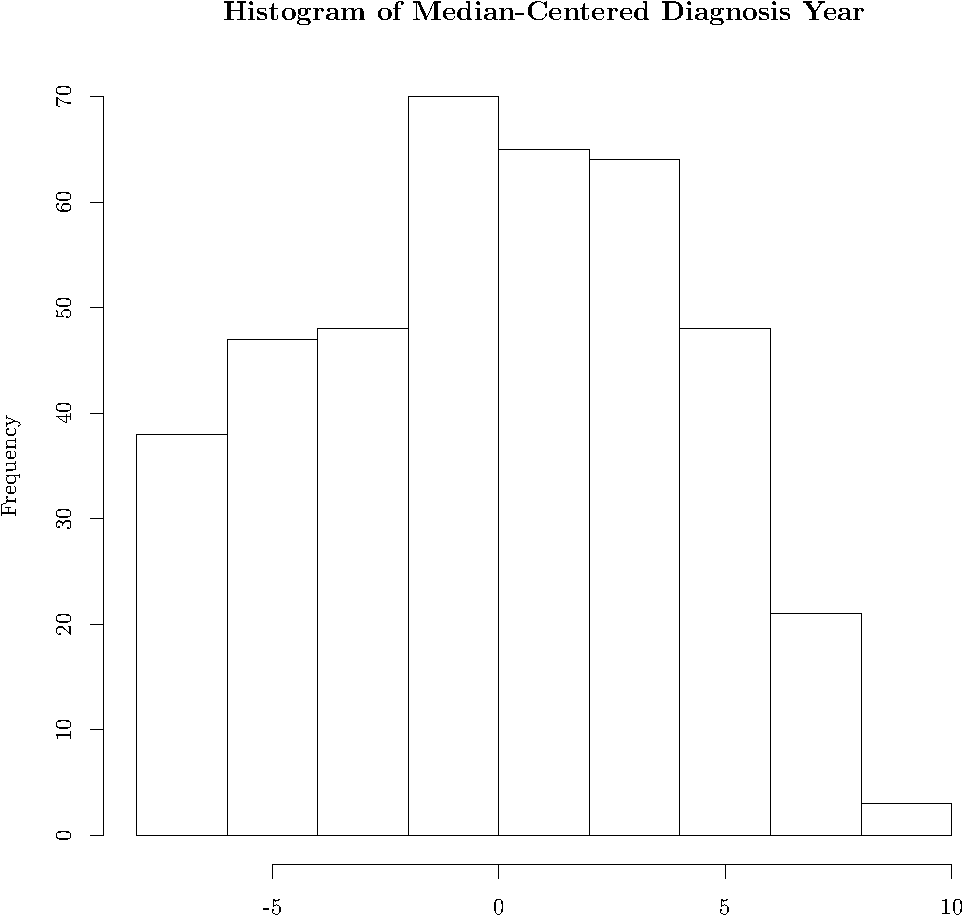
\includegraphics[width=\maxwidth]{figure/05-data-selection-1} 

}


\begin{kframe}\begin{alltt}
\hlstd{y} \hlkwb{=} \hlkwd{Surv}\hlstd{(}\hlkwd{as.numeric}\hlstd{(data}\hlopt{$}\hlstd{History.Death.Date} \hlopt{-} \hlstd{data}\hlopt{$}\hlstd{History.Diagnosis.Date), data}\hlopt{$}\hlstd{History.DSDeath.Event)}
\hlcom{# Note no surgery dates, though for almost all pts there were only a few days difference.}

\hlstd{temp} \hlkwb{=} \hlnum{NA}
\hlstd{temp} \hlkwb{=} \hlkwd{ls}\hlstd{()}
\hlkwd{rm}\hlstd{(}\hlkwc{list} \hlstd{= temp[}\hlopt{!}\hlstd{(temp} \hlopt \hlkwd{c}\hlstd{(}\hlstr{"x"}\hlstd{,} \hlstr{"y"}\hlstd{,} \hlstr{"pal"}\hlstd{))])}

\hlstd{sel} \hlkwb{=} \hlopt{!}\hlkwd{is.na}\hlstd{(y[,}\hlnum{1}\hlstd{])} \hlopt{& !}\hlkwd{is.na}\hlstd{(y[,}\hlnum{2}\hlstd{])} \hlopt{& !}\hlkwd{is.na}\hlstd{(x}\hlopt{$}\hlstd{A2)} \hlopt{& !}\hlkwd{is.na}\hlstd{(x}\hlopt{$}\hlstd{A4)} \hlopt{& !}\hlkwd{is.na}\hlstd{(x}\hlopt{$}\hlstd{LocBody)}
\hlstd{x} \hlkwb{=} \hlstd{x[sel,]}
\hlstd{y} \hlkwb{=} \hlstd{y[sel,]}
\hlkwd{rm}\hlstd{(sel)}

\hlcom{# Remove CA-19-9 measurements as they're mostly missing}
\hlstd{x} \hlkwb{=} \hlstd{x[,}\hlkwd{colnames}\hlstd{(x)} \hlopt{!=} \hlstr{"Ca199"}\hlstd{]}

\hlstd{data} \hlkwb{=} \hlkwd{as.data.frame}\hlstd{(}\hlkwd{cbind}\hlstd{(}\hlkwc{Time} \hlstd{= y[,}\hlnum{1}\hlstd{],} \hlkwc{DSD} \hlstd{= y[,}\hlnum{2}\hlstd{], x))}
\hlkwd{rm}\hlstd{(x, y)}
\hlstd{data}\hlopt{$}\hlstd{DSD} \hlkwb{=} \hlstd{data}\hlopt{$}\hlstd{DSD} \hlopt{==} \hlnum{1}

\hlcom{# Remove long-survivors.  These are very likely to be misdiagnoses, or LTF.}
\hlkwd{nrow}\hlstd{(data)}
\end{alltt}
\begin{verbatim}
## [1] 256
\end{verbatim}
\begin{alltt}
\hlstd{data} \hlkwb{=} \hlstd{data[data}\hlopt{$}\hlstd{Time} \hlopt{<} \hlnum{3000}\hlstd{,]}
\hlkwd{nrow}\hlstd{(data)}
\end{alltt}
\begin{verbatim}
## [1] 249
\end{verbatim}
\end{kframe}
\end{knitrout}


%%%%%%%%%%%%%%%%%%%%%%%%%%%%%%%%%%%%%%%%%%%%%%%%%%%%%%%%%%%%%%%%%%%%%%
% DATA SPLITTING
%%%%%%%%%%%%%%%%%%%%%%%%%%%%%%%%%%%%%%%%%%%%%%%%%%%%%%%%%%%%%%%%%%%%%%
\section{Data splitting}
There's going to be an awful lot of model manipulation and black magic going on.  Create a holdout validation set for final model comparison and selection.
\begin{knitrout}
\definecolor{shadecolor}{rgb}{0.969, 0.969, 0.969}\color{fgcolor}\begin{kframe}
\begin{alltt}
\hlkwd{set.seed}\hlstd{(}\hlnum{20150201}\hlstd{)}
\hlstd{sel.val} \hlkwb{=} \hlkwd{sample.int}\hlstd{(}\hlkwd{nrow}\hlstd{(data),} \hlkwd{floor}\hlstd{(}\hlkwd{nrow}\hlstd{(data)}\hlopt{/}\hlnum{5}\hlstd{))}
\hlstd{sel.val} \hlkwb{=} \hlnum{1}\hlopt{:}\hlkwd{nrow}\hlstd{(data)} \hlopt \hlstd{sel.val}
\hlkwd{mean}\hlstd{(sel.val)}
\end{alltt}
\begin{verbatim}
## [1] 0.1968
\end{verbatim}
\begin{alltt}
\hlstd{data.val} \hlkwb{=} \hlstd{data[sel.val,,}\hlkwc{drop} \hlstd{=} \hlnum{FALSE}\hlstd{]}
\hlstd{data} \hlkwb{=} \hlstd{data[}\hlopt{!}\hlstd{sel.val,,}\hlkwc{drop} \hlstd{=} \hlnum{FALSE}\hlstd{]}
\hlkwd{nrow}\hlstd{(data)}
\end{alltt}
\begin{verbatim}
## [1] 200
\end{verbatim}
\begin{alltt}
\hlkwd{nrow}\hlstd{(data.val)}
\end{alltt}
\begin{verbatim}
## [1] 49
\end{verbatim}
\end{kframe}
\end{knitrout}


%%%%%%%%%%%%%%%%%%%%%%%%%%%%%%%%%%%%%%%%%%%%%%%%%%%%%%%%%%%%%%%%%%%%%%
% MODEL SPECIFICATION
%%%%%%%%%%%%%%%%%%%%%%%%%%%%%%%%%%%%%%%%%%%%%%%%%%%%%%%%%%%%%%%%%%%%%%
\section{EDA}
Use the CPH model as a convenient framework for EDA.
\subsection{Functional form}
Investigate functional form with martingale residuals.
\begin{knitrout}
\definecolor{shadecolor}{rgb}{0.969, 0.969, 0.969}\color{fgcolor}\begin{kframe}
\begin{alltt}
\hlstd{fit.cph.NoAge} \hlkwb{=} \hlkwd{coxph}\hlstd{(}\hlkwd{Surv}\hlstd{(Time, DSD)} \hlopt{~} \hlstd{DiagYearCent} \hlopt{+} \hlstd{SexM} \hlopt{+} \hlstd{LocBody} \hlopt{+} \hlstd{SizeCent} \hlopt{+} \hlstd{A2} \hlopt{+} \hlstd{A4,} \hlkwc{data} \hlstd{= data)}
\hlkwd{scatter.smooth}\hlstd{(data}\hlopt{$}\hlstd{AgeCent,} \hlkwd{resid}\hlstd{(fit.cph.NoAge,} \hlkwc{type} \hlstd{=} \hlstr{"martingale"}\hlstd{),} \hlkwc{xlab} \hlstd{=} \hlstr{""}\hlstd{,} \hlkwc{ylab} \hlstd{=} \hlstr{"Martingale residual"}\hlstd{)}
\end{alltt}
\end{kframe}

{\centering 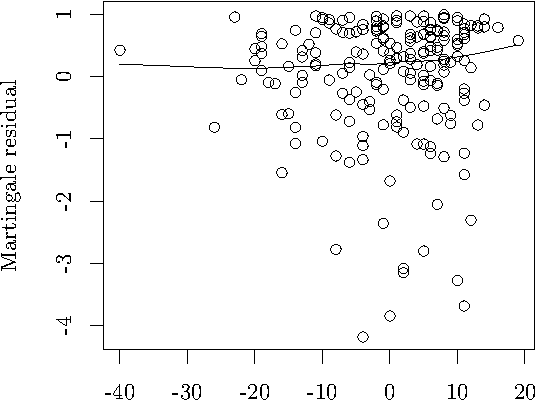
\includegraphics[width=\maxwidth]{figure/05-eda-func-form-age-1} 

}


\begin{kframe}\begin{alltt}
\hlkwd{scatter.smooth}\hlstd{(data}\hlopt{$}\hlstd{AgeCent,} \hlkwd{resid}\hlstd{(fit.cph.NoAge,} \hlkwc{type} \hlstd{=} \hlstr{"martingale"}\hlstd{),} \hlkwc{xlab} \hlstd{=} \hlstr{""}\hlstd{,} \hlkwc{ylab} \hlstd{=} \hlstr{"Martingale residual"}\hlstd{,} \hlkwc{ylim} \hlstd{=} \hlkwd{c}\hlstd{(}\hlopt{-}\hlnum{1}\hlstd{,} \hlnum{1}\hlstd{))}
\end{alltt}
\end{kframe}

{\centering 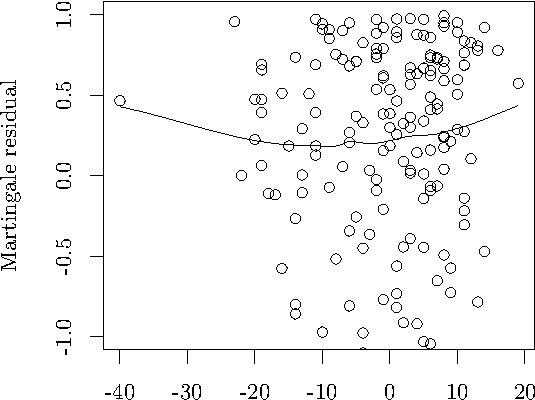
\includegraphics[width=\maxwidth]{figure/05-eda-func-form-age-2} 

}



\end{knitrout}
Close enough to linear.

\begin{knitrout}
\definecolor{shadecolor}{rgb}{0.969, 0.969, 0.969}\color{fgcolor}\begin{kframe}
\begin{alltt}
\hlstd{fit.cph.NoDate} \hlkwb{=} \hlkwd{coxph}\hlstd{(}\hlkwd{Surv}\hlstd{(Time, DSD)} \hlopt{~} \hlstd{SexM} \hlopt{+} \hlstd{AgeCent} \hlopt{+} \hlstd{LocBody} \hlopt{+} \hlstd{SizeCent} \hlopt{+} \hlstd{A2} \hlopt{+} \hlstd{A4,} \hlkwc{data} \hlstd{= data)}
\hlkwd{scatter.smooth}\hlstd{(data}\hlopt{$}\hlstd{DiagYearCent,} \hlkwd{resid}\hlstd{(fit.cph.NoDate,} \hlkwc{type} \hlstd{=} \hlstr{"martingale"}\hlstd{),} \hlkwc{xlab} \hlstd{=} \hlstr{""}\hlstd{,} \hlkwc{ylab} \hlstd{=} \hlstr{"Martingale residual"}\hlstd{)}
\end{alltt}
\end{kframe}

{\centering 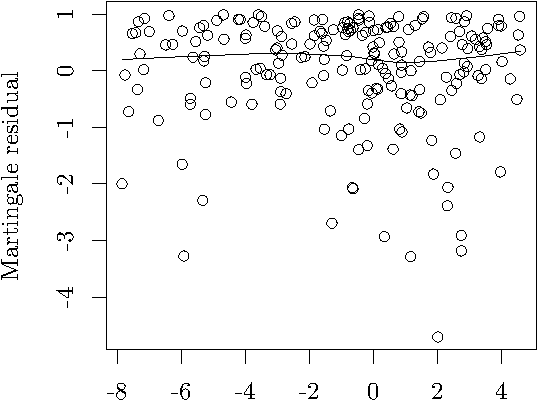
\includegraphics[width=\maxwidth]{figure/05-eda-func-form-date-1} 

}


\begin{kframe}\begin{alltt}
\hlkwd{scatter.smooth}\hlstd{(data}\hlopt{$}\hlstd{DiagYearCent,} \hlkwd{resid}\hlstd{(fit.cph.NoDate,} \hlkwc{type} \hlstd{=} \hlstr{"martingale"}\hlstd{),} \hlkwc{xlab} \hlstd{=} \hlstr{""}\hlstd{,} \hlkwc{ylab} \hlstd{=} \hlstr{"Martingale residual"}\hlstd{,} \hlkwc{ylim} \hlstd{=} \hlkwd{c}\hlstd{(}\hlopt{-}\hlnum{1}\hlstd{,} \hlnum{1}\hlstd{))}
\end{alltt}
\end{kframe}

{\centering 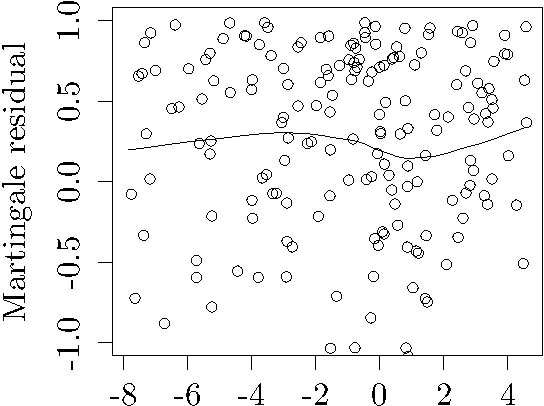
\includegraphics[width=\maxwidth]{figure/05-eda-func-form-date-2} 

}



\end{knitrout}
Doesn't appear to have much of an effect.

\begin{knitrout}
\definecolor{shadecolor}{rgb}{0.969, 0.969, 0.969}\color{fgcolor}\begin{kframe}
\begin{alltt}
\hlstd{fit.cph.NoSize} \hlkwb{=} \hlkwd{coxph}\hlstd{(}\hlkwd{Surv}\hlstd{(Time, DSD)} \hlopt{~} \hlstd{DiagYearCent} \hlopt{+} \hlstd{SexM} \hlopt{+} \hlstd{AgeCent} \hlopt{+} \hlstd{LocBody} \hlopt{+} \hlstd{A2} \hlopt{+} \hlstd{A4,} \hlkwc{data} \hlstd{= data)}
\hlkwd{scatter.smooth}\hlstd{(data}\hlopt{$}\hlstd{SizeCent,} \hlkwd{resid}\hlstd{(fit.cph.NoSize,} \hlkwc{type} \hlstd{=} \hlstr{"martingale"}\hlstd{),} \hlkwc{xlab} \hlstd{=} \hlstr{""}\hlstd{,} \hlkwc{ylab} \hlstd{=} \hlstr{"Martingale residual"}\hlstd{)}
\end{alltt}
\end{kframe}

{\centering 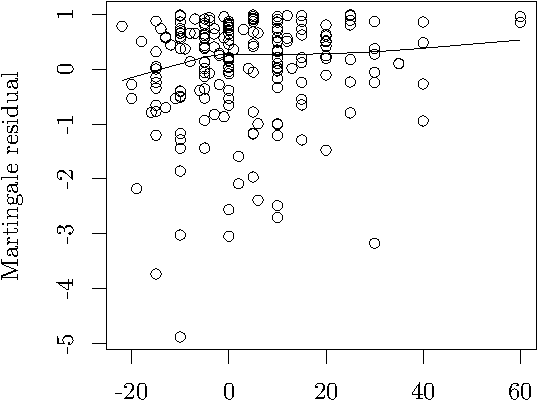
\includegraphics[width=\maxwidth]{figure/05-eda-func-form-size-1} 

}


\begin{kframe}\begin{alltt}
\hlkwd{scatter.smooth}\hlstd{(data}\hlopt{$}\hlstd{SizeCent,} \hlkwd{resid}\hlstd{(fit.cph.NoSize,} \hlkwc{type} \hlstd{=} \hlstr{"martingale"}\hlstd{),} \hlkwc{xlab} \hlstd{=} \hlstr{""}\hlstd{,} \hlkwc{ylab} \hlstd{=} \hlstr{"Martingale residual"}\hlstd{,} \hlkwc{ylim} \hlstd{=} \hlkwd{c}\hlstd{(}\hlopt{-}\hlnum{1}\hlstd{,} \hlnum{1}\hlstd{))}
\end{alltt}
\end{kframe}

{\centering 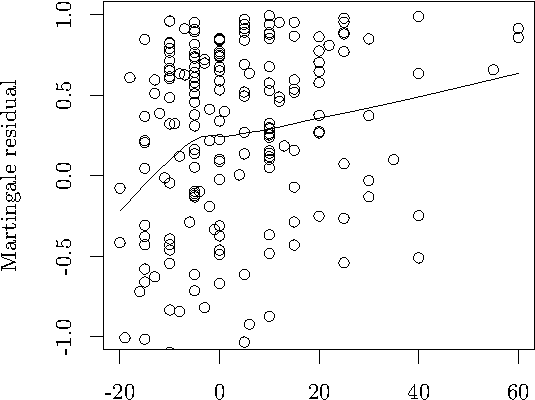
\includegraphics[width=\maxwidth]{figure/05-eda-func-form-size-2} 

}



\end{knitrout}
The size relationship appears to have a knee, close to size == 0, around which the relationship is approximately linear.

Model size as: $SizeCent + SizeCent I(SizeCent > 0) \equiv SizeCent + SizeCent_+$

\begin{knitrout}
\definecolor{shadecolor}{rgb}{0.969, 0.969, 0.969}\color{fgcolor}\begin{kframe}
\begin{alltt}
\hlstd{data}\hlopt{$}\hlstd{SizePlus} \hlkwb{=} \hlkwd{pmax}\hlstd{(data}\hlopt{$}\hlstd{SizeCent,} \hlnum{0}\hlstd{)}
\hlstd{data.val}\hlopt{$}\hlstd{SizePlus} \hlkwb{=} \hlkwd{pmax}\hlstd{(data.val}\hlopt{$}\hlstd{SizeCent,} \hlnum{0}\hlstd{)}
\end{alltt}
\end{kframe}
\end{knitrout}


\subsection{PH assumption: full model}
\begin{knitrout}
\definecolor{shadecolor}{rgb}{0.969, 0.969, 0.969}\color{fgcolor}\begin{kframe}
\begin{alltt}
\hlstd{fit.cph} \hlkwb{=} \hlkwd{coxph}\hlstd{(}\hlkwd{Surv}\hlstd{(Time, DSD)} \hlopt{~} \hlstd{SexM} \hlopt{+} \hlstd{AgeCent} \hlopt{+} \hlstd{LocBody} \hlopt{+} \hlstd{SizeCent} \hlopt{+} \hlstd{SizePlus} \hlopt{+} \hlstd{A2} \hlopt{+} \hlstd{A4,} \hlkwc{data} \hlstd{= data)}
\hlkwd{cox.zph}\hlstd{(fit.cph)}
\end{alltt}
\begin{verbatim}
##                  rho    chisq      p
## SexMTRUE     0.17964  6.56115 0.0104
## AgeCent     -0.10574  2.40668 0.1208
## LocBodyTRUE -0.04856  0.37895 0.5382
## SizeCent     0.00231  0.00106 0.9740
## SizePlus    -0.01130  0.02666 0.8703
## A2TRUE      -0.03995  0.29907 0.5845
## A4TRUE      -0.08343  1.33308 0.2483
## GLOBAL            NA 13.17267 0.0680
\end{verbatim}
\begin{alltt}
\hlstd{fit.cph} \hlkwb{=} \hlkwd{coxph}\hlstd{(}\hlkwd{Surv}\hlstd{(Time, DSD)} \hlopt{~} \hlkwd{strata}\hlstd{(SexM)} \hlopt{+} \hlstd{AgeCent} \hlopt{+} \hlstd{LocBody} \hlopt{+} \hlstd{SizeCent} \hlopt{+} \hlstd{SizePlus} \hlopt{+} \hlstd{A2} \hlopt{+} \hlstd{A4,} \hlkwc{data} \hlstd{= data)}
\hlkwd{cox.zph}\hlstd{(fit.cph)}
\end{alltt}
\begin{verbatim}
##                  rho   chisq      p
## AgeCent     -0.11339 2.78186 0.0953
## LocBodyTRUE -0.04618 0.34177 0.5588
## SizeCent     0.00662 0.00857 0.9262
## SizePlus    -0.01329 0.03588 0.8498
## A2TRUE      -0.04361 0.35772 0.5498
## A4TRUE      -0.07985 1.25354 0.2629
## GLOBAL            NA 6.03352 0.4194
\end{verbatim}
\end{kframe}
\end{knitrout}
Using a threshold of 0.1 for the CPH tests, sex is stuffing things up.  Stratification by sex makes good sense, given known variation in survival between the sexes.  It would have been possible to model this with a Sex:Age term in an AFT model, but given this is CPH, a baseline change is needed.


\subsection{Date of diagnosis test}
\begin{knitrout}
\definecolor{shadecolor}{rgb}{0.969, 0.969, 0.969}\color{fgcolor}\begin{kframe}
\begin{alltt}
\hlstd{temp1} \hlkwb{=} \hlkwd{coxph}\hlstd{(}\hlkwd{Surv}\hlstd{(Time, DSD)} \hlopt{~} \hlkwd{strata}\hlstd{(SexM)} \hlopt{+} \hlstd{AgeCent} \hlopt{+} \hlstd{LocBody} \hlopt{+} \hlstd{SizeCent} \hlopt{+} \hlstd{SizePlus} \hlopt{+} \hlstd{A2} \hlopt{+} \hlstd{A4,} \hlkwc{data} \hlstd{= data)}
\hlstd{temp2} \hlkwb{=} \hlkwd{coxph}\hlstd{(}\hlkwd{Surv}\hlstd{(Time, DSD)} \hlopt{~} \hlkwd{strata}\hlstd{(SexM)} \hlopt{+} \hlstd{AgeCent} \hlopt{+} \hlstd{LocBody} \hlopt{+} \hlstd{SizeCent} \hlopt{+} \hlstd{SizePlus} \hlopt{+} \hlstd{A2} \hlopt{+} \hlstd{A4} \hlopt{+} \hlstd{DiagYearCent,} \hlkwc{data} \hlstd{= data)}
\hlkwd{anova}\hlstd{(temp1, temp2)}
\end{alltt}
\begin{verbatim}
## Analysis of Deviance Table
##  Cox model: response is  Surv(Time, DSD)
##  Model 1: ~ strata(SexM) + AgeCent + LocBody + SizeCent + SizePlus + A2 + A4
##  Model 2: ~ strata(SexM) + AgeCent + LocBody + SizeCent + SizePlus + A2 + A4 + DiagYearCent
##   loglik Chisq Df P(>|Chi|)
## 1   -682                   
## 2   -682  0.86  1      0.35
\end{verbatim}
\end{kframe}
\end{knitrout}
Not significant; good.


\subsection{Outliers}
\begin{knitrout}
\definecolor{shadecolor}{rgb}{0.969, 0.969, 0.969}\color{fgcolor}\begin{kframe}
\begin{alltt}
\hlkwd{plot}\hlstd{(}\hlkwd{resid}\hlstd{(fit.cph,} \hlstr{"deviance"}\hlstd{))}
\hlkwd{abline}\hlstd{(}\hlkwc{h} \hlstd{=} \hlkwd{c}\hlstd{(}\hlopt{-}\hlnum{2}\hlstd{,} \hlnum{2}\hlstd{))}
\end{alltt}
\end{kframe}

{\centering 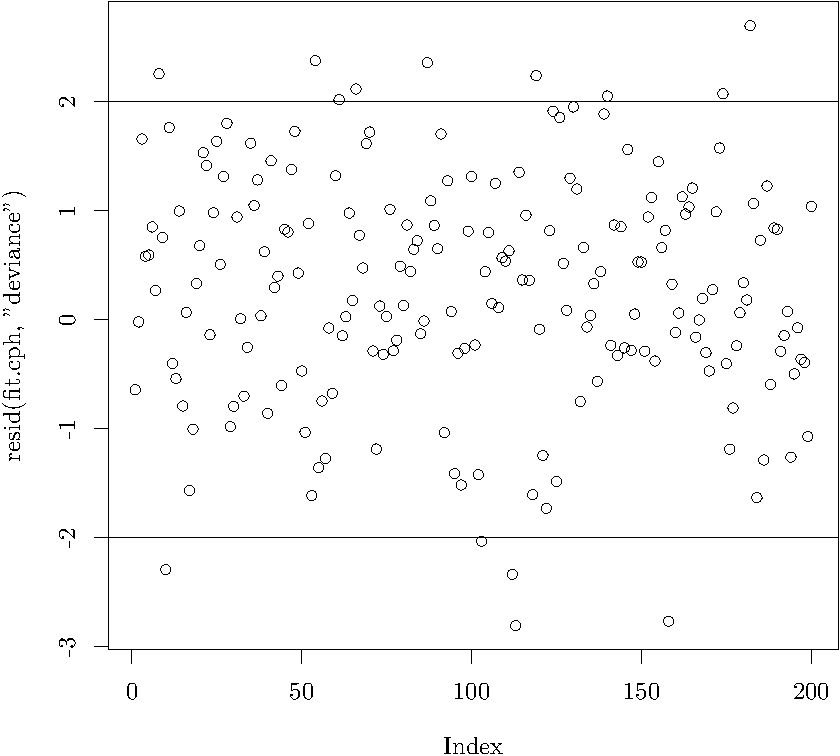
\includegraphics[width=\maxwidth]{figure/05-eda-outliers-1} 

}


\begin{kframe}\begin{alltt}
\hlstd{data}\hlopt{$}\hlstd{devresid} \hlkwb{=} \hlkwd{resid}\hlstd{(fit.cph,} \hlkwc{type} \hlstd{=} \hlstr{"deviance"}\hlstd{)}
\hlstd{temp} \hlkwb{=} \hlstd{data[}\hlkwd{abs}\hlstd{(data}\hlopt{$}\hlstd{devresid)} \hlopt{>=} \hlnum{2}\hlstd{,]}
\hlstd{temp[}\hlkwd{order}\hlstd{(temp}\hlopt{$}\hlstd{Time),]}
\end{alltt}
\begin{verbatim}
##             Time   DSD DiagYearCent  SexM AgeCent LocBody SizeCent    A2
## NSWPCN_315    26  TRUE      -0.4627  TRUE       3    TRUE       25  TRUE
## NSWPCN_374    63  TRUE      -3.5921  TRUE       5   FALSE      -10  TRUE
## NSWPCN_1177   68  TRUE      -4.6845 FALSE       1   FALSE        5 FALSE
## NSWPCN_333    90  TRUE      -0.1396  TRUE      10    TRUE       25 FALSE
## NSWPCN_779    96  TRUE       2.9076 FALSE       3   FALSE       12 FALSE
## NSWPCN_1165   97  TRUE       4.5640  TRUE      -6   FALSE       15 FALSE
## NSWPCN_324   100  TRUE       1.5688 FALSE     -10   FALSE       10 FALSE
## NSWPCN_1017  100  TRUE      -3.4908 FALSE      -5   FALSE        5 FALSE
## NSWPCN_125   103  TRUE      -6.3847 FALSE      -2   FALSE      -10 FALSE
## NSWPCN_133  1304 FALSE      -5.3279  TRUE       5   FALSE        6 FALSE
## NSWPCN_655  1723  TRUE       0.3368  TRUE      11    TRUE       10 FALSE
## NSWPCN_1095 1836 FALSE       2.7461  TRUE      -8   FALSE        0  TRUE
## NSWPCN_668  2106 FALSE       2.0068 FALSE      -2   FALSE       30 FALSE
## NSWPCN_667  2415 FALSE       1.1608 FALSE     -14   FALSE      -15 FALSE
##                A4 SizePlus devresid
## NSWPCN_315   TRUE       25    2.379
## NSWPCN_374   TRUE        0    2.361
## NSWPCN_1177  TRUE        5    2.701
## NSWPCN_333   TRUE       25    2.119
## NSWPCN_779   TRUE       12    2.243
## NSWPCN_1165  TRUE       15    2.076
## NSWPCN_324   TRUE       10    2.022
## NSWPCN_1017  TRUE        5    2.055
## NSWPCN_125  FALSE        0    2.260
## NSWPCN_133   TRUE        6   -2.292
## NSWPCN_655   TRUE       10   -2.031
## NSWPCN_1095 FALSE        0   -2.765
## NSWPCN_668   TRUE       30   -2.806
## NSWPCN_667   TRUE        0   -2.336
\end{verbatim}
\begin{alltt}
\hlstd{temp} \hlkwb{=} \hlkwd{resid}\hlstd{(fit.cph,} \hlkwc{type} \hlstd{=} \hlstr{"dfbetas"}\hlstd{)}
\hlkwd{colnames}\hlstd{(temp)} \hlkwb{=} \hlkwd{names}\hlstd{(fit.cph}\hlopt{$}\hlstd{coefficients)}
\hlstd{temp} \hlkwb{=} \hlkwd{melt}\hlstd{(temp)}
\hlkwd{colnames}\hlstd{(temp)} \hlkwb{=} \hlkwd{c}\hlstd{(}\hlstr{"Patient"}\hlstd{,} \hlstr{"Coefficient"}\hlstd{,} \hlstr{"dfbetas"}\hlstd{)}
\hlstd{temp}\hlopt{$}\hlstd{Patient} \hlkwb{=} \hlkwd{gsub}\hlstd{(}\hlstr{"NSWPCN_"}\hlstd{,} \hlstr{""}\hlstd{, temp}\hlopt{$}\hlstd{Patient)}
\hlnum{2}\hlopt{/}\hlkwd{sqrt}\hlstd{(}\hlkwd{nrow}\hlstd{(data))}              \hlcom{# The classic threshold for concern is 2/sqrt(n).}
\end{alltt}
\begin{verbatim}
## [1] 0.1414
\end{verbatim}
\begin{alltt}
\hlkwd{ggplot}\hlstd{(temp,} \hlkwd{aes}\hlstd{(}\hlkwc{y} \hlstd{=} \hlkwd{abs}\hlstd{(dfbetas),} \hlkwc{x} \hlstd{= Patient,} \hlkwc{col} \hlstd{= Coefficient))} \hlopt{+} \hlkwd{geom_point}\hlstd{()} \hlopt{+} \hlkwd{geom_hline}\hlstd{(}\hlkwc{yintercept} \hlstd{=} \hlnum{2}\hlopt{/}\hlkwd{sqrt}\hlstd{(}\hlkwd{nrow}\hlstd{(data)))}
\end{alltt}
\end{kframe}

{\centering 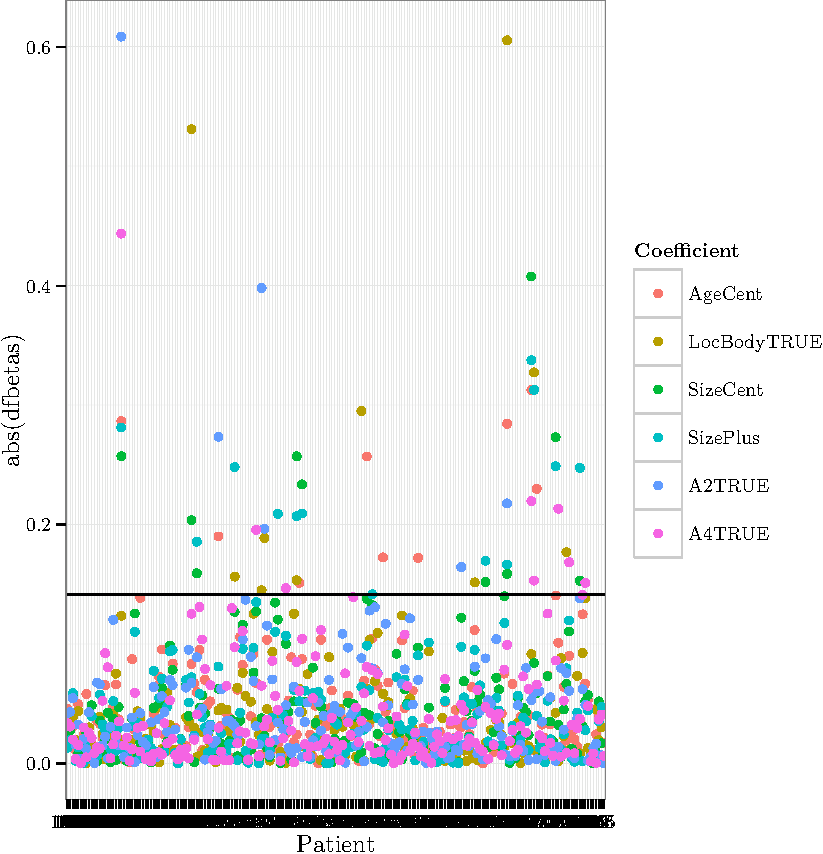
\includegraphics[width=\maxwidth]{figure/05-eda-outliers-2} 

}


\begin{kframe}\begin{alltt}
\hlkwd{sort}\hlstd{(}\hlkwd{apply}\hlstd{(}\hlkwd{abs}\hlstd{(}\hlkwd{resid}\hlstd{(fit.cph,} \hlkwc{type} \hlstd{=} \hlstr{"dfbetas"}\hlstd{)),} \hlnum{1}\hlstd{, max),} \hlkwc{decreasing} \hlstd{=} \hlnum{TRUE}\hlstd{)}
\end{alltt}
\begin{verbatim}
## NSWPCN_1095  NSWPCN_655 NSWPCN_1182  NSWPCN_667  NSWPCN_144  NSWPCN_668 
##    0.608593    0.605502    0.530888    0.407716    0.398158    0.327457 
##  NSWPCN_310 NSWPCN_1212  NSWPCN_784  NSWPCN_192  NSWPCN_313 NSWPCN_1253 
##    0.295058    0.273608    0.273058    0.257139    0.257021    0.248100 
##  NSWPCN_799  NSWPCN_195  NSWPCN_674  NSWPCN_788  NSWPCN_154  NSWPCN_145 
##    0.247494    0.233634    0.229905    0.213230    0.209001    0.196503 
##  NSWPCN_142 NSWPCN_1186  NSWPCN_794  NSWPCN_320  NSWPCN_349  NSWPCN_639 
##    0.195590    0.185655    0.176847    0.172566    0.172120    0.169714 
##  NSWPCN_795  NSWPCN_374  NSWPCN_445  NSWPCN_802  NSWPCN_194  NSWPCN_163 
##    0.168470    0.164443    0.151616    0.151183    0.151178    0.146712 
##  NSWPCN_316  NSWPCN_801  NSWPCN_654  NSWPCN_307 NSWPCN_1147  NSWPCN_135 
##    0.141622    0.141212    0.139981    0.139227    0.138642    0.137147 
##  NSWPCN_152 NSWPCN_1187  NSWPCN_317  NSWPCN_125  NSWPCN_315 NSWPCN_1145 
##    0.134638    0.131048    0.130750    0.129984    0.127999    0.125567 
##  NSWPCN_777  NSWPCN_141  NSWPCN_182  NSWPCN_333  NSWPCN_337 NSWPCN_1083 
##    0.125524    0.125370    0.125309    0.123862    0.121565    0.120246 
##  NSWPCN_321  NSWPCN_133 NSWPCN_1453  NSWPCN_269  NSWPCN_318  NSWPCN_296 
##    0.116968    0.116092    0.115398    0.111797    0.109297    0.108507 
##  NSWPCN_335  NSWPCN_132  NSWPCN_647 NSWPCN_1188  NSWPCN_354 NSWPCN_1168 
##    0.107926    0.105932    0.104040    0.103771    0.101211    0.098668 
##  NSWPCN_305 NSWPCN_1160 NSWPCN_1179 NSWPCN_1169  NSWPCN_151 NSWPCN_1071 
##    0.096994    0.095425    0.095199    0.095118    0.093520    0.092355 
##  NSWPCN_331  NSWPCN_267  NSWPCN_138  NSWPCN_276   NSWPCN_17  NSWPCN_789 
##    0.091974    0.089754    0.089265    0.089051    0.088914    0.088141 
## NSWPCN_1141 NSWPCN_1072  NSWPCN_257  NSWPCN_664 NSWPCN_1189 NSWPCN_1155 
##    0.087304    0.080513    0.080219    0.079865    0.079050    0.077529 
##  NSWPCN_303 NSWPCN_1088  NSWPCN_200  NSWPCN_798  NSWPCN_663 NSWPCN_1158 
##    0.075390    0.075103    0.074720    0.073281    0.072910    0.072736 
##  NSWPCN_364 NSWPCN_1177  NSWPCN_312  NSWPCN_375  NSWPCN_324 NSWPCN_1028 
##    0.070600    0.069807    0.069320    0.068858    0.067746    0.067618 
## NSWPCN_1183  NSWPCN_657 NSWPCN_1031 NSWPCN_1198  NSWPCN_637 NSWPCN_1222 
##    0.067251    0.066525    0.066068    0.065549    0.065423    0.065069 
##  NSWPCN_336 NSWPCN_1157  NSWPCN_790    NSWPCN_4   NSWPCN_13  NSWPCN_665 
##    0.064764    0.064604    0.064267    0.063796    0.063341    0.062318 
## NSWPCN_1213  NSWPCN_648  NSWPCN_636  NSWPCN_281   NSWPCN_20  NSWPCN_347 
##    0.062295    0.062010    0.061429    0.061039    0.060975    0.060948 
##  NSWPCN_769  NSWPCN_268 NSWPCN_1167 NSWPCN_1017 NSWPCN_1022  NSWPCN_804 
##    0.060504    0.059817    0.059415    0.058835    0.058110    0.057379 
##  NSWPCN_661  NSWPCN_779  NSWPCN_640  NSWPCN_164 NSWPCN_1066  NSWPCN_813 
##    0.056829    0.055459    0.052953    0.052737    0.052580    0.051966 
## NSWPCN_1165  NSWPCN_643 NSWPCN_1019 NSWPCN_1190  NSWPCN_376 NSWPCN_1026 
##    0.051250    0.049904    0.049674    0.049013    0.048787    0.048713 
##  NSWPCN_282  NSWPCN_815 NSWPCN_1089  NSWPCN_308  NSWPCN_284   NSWPCN_10 
##    0.048235    0.047547    0.047147    0.046789    0.046011    0.045675 
##  NSWPCN_811  NSWPCN_372 NSWPCN_1146 NSWPCN_1016 NSWPCN_1023  NSWPCN_653 
##    0.045397    0.044821    0.043795    0.043085    0.042856    0.041802 
##  NSWPCN_283  NSWPCN_270  NSWPCN_162  NSWPCN_306  NSWPCN_662  NSWPCN_363 
##    0.041402    0.040900    0.040385    0.040045    0.039252    0.038086 
## NSWPCN_1227  NSWPCN_369  NSWPCN_770 NSWPCN_1153  NSWPCN_796  NSWPCN_332 
##    0.038003    0.035265    0.034983    0.034467    0.032432    0.032422 
##  NSWPCN_373 NSWPCN_1148  NSWPCN_272 NSWPCN_1075  NSWPCN_149 NSWPCN_1139 
##    0.032184    0.031468    0.031391    0.030774    0.030526    0.030104 
## NSWPCN_1021  NSWPCN_352 NSWPCN_1171  NSWPCN_325  NSWPCN_362  NSWPCN_360 
##    0.030095    0.030008    0.029728    0.027767    0.026652    0.026516 
##  NSWPCN_309  NSWPCN_646  NSWPCN_348   NSWPCN_36  NSWPCN_384  NSWPCN_256 
##    0.026444    0.026071    0.025947    0.025334    0.024514    0.024298 
##  NSWPCN_143  NSWPCN_319  NSWPCN_366  NSWPCN_358  NSWPCN_775  NSWPCN_370 
##    0.023931    0.022670    0.022058    0.021289    0.021157    0.021082 
## NSWPCN_1150 NSWPCN_1175  NSWPCN_797 NSWPCN_1152  NSWPCN_350 NSWPCN_1018 
##    0.020619    0.020474    0.020089    0.019960    0.019915    0.019881 
## NSWPCN_1211  NSWPCN_656  NSWPCN_781    NSWPCN_9 NSWPCN_1207  NSWPCN_658 
##    0.018856    0.018714    0.018620    0.017311    0.017230    0.016422 
## NSWPCN_1176 NSWPCN_1136  NSWPCN_807 NSWPCN_1140 NSWPCN_1027 NSWPCN_1173 
##    0.015073    0.014981    0.013112    0.012942    0.011384    0.011157 
## NSWPCN_1215  NSWPCN_638 NSWPCN_1020  NSWPCN_330  NSWPCN_157  NSWPCN_353 
##    0.010917    0.010175    0.010018    0.009944    0.009637    0.008259 
##  NSWPCN_806  NSWPCN_136 
##    0.007888    0.003489
\end{verbatim}
\begin{alltt}
\hlkwd{sum}\hlstd{(}\hlkwd{apply}\hlstd{(}\hlkwd{abs}\hlstd{(}\hlkwd{resid}\hlstd{(fit.cph,} \hlkwc{type} \hlstd{=} \hlstr{"dfbetas"}\hlstd{)),} \hlnum{1}\hlstd{, max)} \hlopt{>} \hlnum{2}\hlopt{/}\hlkwd{sqrt}\hlstd{(}\hlkwd{nrow}\hlstd{(data)))}
\end{alltt}
\begin{verbatim}
## [1] 31
\end{verbatim}
\begin{alltt}
\hlstd{temp} \hlkwb{=} \hlkwd{resid}\hlstd{(fit.cph,} \hlkwc{type} \hlstd{=} \hlstr{"dfbetas"}\hlstd{)}
\hlstd{data}\hlopt{$}\hlstd{DFBETAS_max} \hlkwb{=} \hlkwd{apply}\hlstd{(}\hlkwd{abs}\hlstd{(temp),} \hlnum{1}\hlstd{, max)}
\hlstd{data}\hlopt{$}\hlstd{DFBETAS_vars} \hlkwb{=} \hlkwd{apply}\hlstd{(}\hlkwd{abs}\hlstd{(temp),} \hlnum{1}\hlstd{,} \hlkwa{function}\hlstd{(}\hlkwc{x}\hlstd{)} \hlkwd{paste}\hlstd{(}\hlkwd{attr}\hlstd{(fit.cph}\hlopt{$}\hlstd{terms,} \hlstr{"term.labels"}\hlstd{)[x} \hlopt{>} \hlnum{2}\hlopt{/}\hlkwd{sqrt}\hlstd{(}\hlkwd{nrow}\hlstd{(data))],} \hlkwc{collapse} \hlstd{=} \hlstr{","}\hlstd{))}
\hlstd{temp} \hlkwb{=} \hlstd{data[data}\hlopt{$}\hlstd{DFBETAS_max} \hlopt{>=} \hlnum{2}\hlopt{/}\hlkwd{sqrt}\hlstd{(}\hlkwd{nrow}\hlstd{(data))} \hlopt{|} \hlkwd{abs}\hlstd{(data}\hlopt{$}\hlstd{devresid)} \hlopt{>=} \hlnum{2}\hlstd{,]}
\hlstd{temp[}\hlkwd{order}\hlstd{(temp}\hlopt{$}\hlstd{DFBETAS_max),]}
\end{alltt}
\begin{verbatim}
##             Time   DSD DiagYearCent  SexM AgeCent LocBody SizeCent    A2
## NSWPCN_1165   97  TRUE       4.5640  TRUE      -6   FALSE       15 FALSE
## NSWPCN_779    96  TRUE       2.9076 FALSE       3   FALSE       12 FALSE
## NSWPCN_1017  100  TRUE      -3.4908 FALSE      -5   FALSE        5 FALSE
## NSWPCN_324   100  TRUE       1.5688 FALSE     -10   FALSE       10 FALSE
## NSWPCN_1177   68  TRUE      -4.6845 FALSE       1   FALSE        5 FALSE
## NSWPCN_133  1304 FALSE      -5.3279  TRUE       5   FALSE        6 FALSE
## NSWPCN_333    90  TRUE      -0.1396  TRUE      10    TRUE       25 FALSE
## NSWPCN_315    26  TRUE      -0.4627  TRUE       3    TRUE       25  TRUE
## NSWPCN_125   103  TRUE      -6.3847 FALSE      -2   FALSE      -10 FALSE
## NSWPCN_316  1698  TRUE      -0.6379 FALSE      -8   FALSE        5 FALSE
## NSWPCN_163   285  TRUE      -2.5544  TRUE      -2   FALSE        0 FALSE
## NSWPCN_194  1123  TRUE      -0.4600 FALSE     -16   FALSE       10 FALSE
## NSWPCN_802  1072  TRUE      -1.0048 FALSE     -14    TRUE       25 FALSE
## NSWPCN_445   114  TRUE       2.5763 FALSE      14    TRUE        5 FALSE
## NSWPCN_374    63  TRUE      -3.5921  TRUE       5   FALSE      -10  TRUE
## NSWPCN_795   128  TRUE       0.7858 FALSE       8   FALSE       -1 FALSE
## NSWPCN_639  1990  TRUE       2.3053 FALSE       1   FALSE        2 FALSE
## NSWPCN_349  1412  TRUE       0.6133  TRUE      11   FALSE        5 FALSE
## NSWPCN_320   804  TRUE      -1.3443 FALSE     -26   FALSE       15 FALSE
## NSWPCN_794   498 FALSE       0.8186 FALSE      -4    TRUE       10 FALSE
## NSWPCN_1186 1892  TRUE      -7.8494 FALSE       2   FALSE        0 FALSE
## NSWPCN_142  1691  TRUE       1.0349  TRUE       4   FALSE        0 FALSE
## NSWPCN_145   599  TRUE       2.5626  TRUE      -6    TRUE       15  TRUE
## NSWPCN_154   163  TRUE      -0.8022  TRUE      -2    TRUE       60 FALSE
## NSWPCN_788  2155 FALSE       1.8727 FALSE       5   FALSE      -10 FALSE
## NSWPCN_674   345  TRUE       3.5647  TRUE     -40   FALSE      -10 FALSE
## NSWPCN_195  1969  TRUE      -0.1889  TRUE       8   FALSE      -16 FALSE
## NSWPCN_799    70  TRUE      -0.4627 FALSE       4    TRUE       60  TRUE
## NSWPCN_1253 1044  TRUE      -5.9713  TRUE      -2   FALSE       40 FALSE
## NSWPCN_313  2521  TRUE      -1.2977 FALSE      12   FALSE      -10 FALSE
## NSWPCN_192   221  TRUE      -0.9008  TRUE      -3    TRUE      -22 FALSE
## NSWPCN_784  2701  TRUE       2.3244  TRUE      14   FALSE      -19 FALSE
## NSWPCN_1212 1053  TRUE       3.9644  TRUE      12   FALSE        2  TRUE
## NSWPCN_310  1093  TRUE       1.8207  TRUE       6    TRUE       -5 FALSE
## NSWPCN_668  2106 FALSE       2.0068 FALSE      -2   FALSE       30 FALSE
## NSWPCN_144  1206  TRUE       2.7379 FALSE       0   FALSE       10  TRUE
## NSWPCN_667  2415 FALSE       1.1608 FALSE     -14   FALSE      -15 FALSE
## NSWPCN_1182 2178  TRUE      -5.9192 FALSE      -4    TRUE      -10 FALSE
## NSWPCN_655  1723  TRUE       0.3368  TRUE      11    TRUE       10 FALSE
## NSWPCN_1095 1836 FALSE       2.7461  TRUE      -8   FALSE        0  TRUE
##                A4 SizePlus devresid DFBETAS_max
## NSWPCN_1165  TRUE       15   2.0759     0.05125
## NSWPCN_779   TRUE       12   2.2425     0.05546
## NSWPCN_1017  TRUE        5   2.0546     0.05884
## NSWPCN_324   TRUE       10   2.0218     0.06775
## NSWPCN_1177  TRUE        5   2.7006     0.06981
## NSWPCN_133   TRUE        6  -2.2919     0.11609
## NSWPCN_333   TRUE       25   2.1193     0.12386
## NSWPCN_315   TRUE       25   2.3787     0.12800
## NSWPCN_125  FALSE        0   2.2600     0.12998
## NSWPCN_316   TRUE        5  -1.3567     0.14162
## NSWPCN_163  FALSE        0   1.6387     0.14671
## NSWPCN_194   TRUE       10  -0.9807     0.15118
## NSWPCN_802  FALSE       25  -0.7492     0.15118
## NSWPCN_445   TRUE        5   1.7057     0.15162
## NSWPCN_374   TRUE        0   2.3607     0.16444
## NSWPCN_795  FALSE        0   1.8566     0.16847
## NSWPCN_639   TRUE        2  -1.4115     0.16971
## NSWPCN_349   TRUE        5  -1.1860     0.17212
## NSWPCN_320   TRUE       15  -0.6732     0.17257
## NSWPCN_794   TRUE       10  -1.4822     0.17685
## NSWPCN_1186  TRUE        0  -1.2863     0.18566
## NSWPCN_142  FALSE        0  -0.7903     0.19559
## NSWPCN_145   TRUE       15  -1.0032     0.19650
## NSWPCN_154   TRUE       60   1.4178     0.20900
## NSWPCN_788  FALSE        0  -1.7288     0.21323
## NSWPCN_674  FALSE        0   1.3545     0.22991
## NSWPCN_195  FALSE        0  -0.7925     0.23363
## NSWPCN_799   TRUE       60   1.9544     0.24749
## NSWPCN_1253  TRUE       40  -1.0703     0.24810
## NSWPCN_313   TRUE        0  -1.6122     0.25702
## NSWPCN_192   TRUE        0   1.8036     0.25714
## NSWPCN_784  FALSE        0  -1.2444     0.27306
## NSWPCN_1212  TRUE        2  -1.2600     0.27361
## NSWPCN_310   TRUE        0  -1.0326     0.29506
## NSWPCN_668   TRUE       30  -2.8060     0.32746
## NSWPCN_144   TRUE       10  -1.5652     0.39816
## NSWPCN_667   TRUE        0  -2.3357     0.40772
## NSWPCN_1182  TRUE        0  -1.6309     0.53089
## NSWPCN_655   TRUE       10  -2.0313     0.60550
## NSWPCN_1095 FALSE        0  -2.7651     0.60859
##                                                  DFBETAS_vars
## NSWPCN_1165                                                  
## NSWPCN_779                                                   
## NSWPCN_1017                                                  
## NSWPCN_324                                                   
## NSWPCN_1177                                                  
## NSWPCN_133                                                   
## NSWPCN_333                                                   
## NSWPCN_315                                                   
## NSWPCN_125                                                   
## NSWPCN_316                                           SizeCent
## NSWPCN_163                                                 A2
## NSWPCN_194                                    strata(SexM),A4
## NSWPCN_802                                                 A2
## NSWPCN_445                                            AgeCent
## NSWPCN_374                                           SizePlus
## NSWPCN_795                                                 A2
## NSWPCN_639                                   LocBody,SizeCent
## NSWPCN_349                                    strata(SexM),A4
## NSWPCN_320                                    strata(SexM),A4
## NSWPCN_794                                            AgeCent
## NSWPCN_1186                                  LocBody,SizeCent
## NSWPCN_142                                                 A2
## NSWPCN_145                                   AgeCent,SizePlus
## NSWPCN_154                                           SizeCent
## NSWPCN_788                                                 A2
## NSWPCN_674                                    strata(SexM),A4
## NSWPCN_195                                   LocBody,SizeCent
## NSWPCN_799                                   LocBody,SizeCent
## NSWPCN_1253                                  AgeCent,SizeCent
## NSWPCN_313                                    strata(SexM),A4
## NSWPCN_192                           AgeCent,LocBody,SizeCent
## NSWPCN_784                                   LocBody,SizeCent
## NSWPCN_1212                          strata(SexM),SizePlus,A4
## NSWPCN_310                                            AgeCent
## NSWPCN_668                                AgeCent,SizeCent,A2
## NSWPCN_144                                   AgeCent,SizePlus
## NSWPCN_667                strata(SexM),LocBody,SizeCent,A2,A4
## NSWPCN_1182                                   AgeCent,LocBody
## NSWPCN_655  strata(SexM),AgeCent,LocBody,SizeCent,SizePlus,A4
## NSWPCN_1095      strata(SexM),LocBody,SizeCent,SizePlus,A2,A4
\end{verbatim}
\end{kframe}
\end{knitrout}

Remove points with deviance residuals > 2.5, or DFBETAS > 0.3.
\begin{knitrout}
\definecolor{shadecolor}{rgb}{0.969, 0.969, 0.969}\color{fgcolor}\begin{kframe}
\begin{alltt}
\hlstd{data} \hlkwb{=} \hlstd{data[data}\hlopt{$}\hlstd{DFBETAS_max} \hlopt{<=} \hlnum{0.3} \hlopt{&} \hlkwd{abs}\hlstd{(data}\hlopt{$}\hlstd{devresid)} \hlopt{<=} \hlnum{2.5}\hlstd{,]}
\hlstd{fit.cph} \hlkwb{=} \hlkwd{coxph}\hlstd{(}\hlkwd{Surv}\hlstd{(Time, DSD)} \hlopt{~} \hlkwd{strata}\hlstd{(SexM)} \hlopt{+} \hlstd{AgeCent} \hlopt{+} \hlstd{LocBody} \hlopt{+} \hlstd{SizeCent} \hlopt{+} \hlstd{SizePlus} \hlopt{+} \hlstd{A2} \hlopt{+} \hlstd{A4,} \hlkwc{data} \hlstd{= data)}
\end{alltt}
\end{kframe}
\end{knitrout}


\subsection{EDA: Variable selection}
\begin{knitrout}
\definecolor{shadecolor}{rgb}{0.969, 0.969, 0.969}\color{fgcolor}\begin{kframe}
\begin{alltt}
\hlstd{nobs.coxph} \hlkwb{<<-} \hlkwa{function}\hlstd{(}\hlkwc{obj}\hlstd{,} \hlkwc{...}\hlstd{)} \hlkwd{sum}\hlstd{(obj}\hlopt{$}\hlstd{y[,}\hlnum{2}\hlstd{])}
\hlkwd{set.seed}\hlstd{(}\hlnum{20150208}\hlstd{)}
\hlstd{fit.cph.as.bic} \hlkwb{=} \hlkwd{glmulti}\hlstd{(}\hlkwd{Surv}\hlstd{(Time, DSD)} \hlopt{~} \hlkwd{strata}\hlstd{(SexM)} \hlopt{+} \hlstd{AgeCent} \hlopt{+} \hlstd{LocBody} \hlopt{+} \hlstd{SizeCent} \hlopt{+} \hlstd{SizePlus} \hlopt{+} \hlstd{A2} \hlopt{+} \hlstd{A4,} \hlkwc{data} \hlstd{= data,} \hlkwc{marginality} \hlstd{=} \hlnum{TRUE}\hlstd{,} \hlkwc{method} \hlstd{=} \hlstr{"g"}\hlstd{,} \hlkwc{fitfunction} \hlstd{=} \hlstr{"coxph"}\hlstd{,} \hlkwc{crit} \hlstd{=} \hlstr{"bic"}\hlstd{,} \hlkwc{level} \hlstd{=} \hlnum{2}\hlstd{,} \hlkwc{plotty} \hlstd{=} \hlnum{FALSE}\hlstd{,} \hlkwc{report} \hlstd{=} \hlnum{TRUE}\hlstd{)}
\end{alltt}
\begin{verbatim}
## Initialization...
## TASK: Genetic algorithm in the candidate set.
## Initialization...
## Algorithm started...
## 
## After 10 generations:
## Best model: Surv(Time,DSD)~1+strata(SexM)+AgeCent+LocBody+SizePlus+A2+A4+SizePlus:LocBody
## Crit= 1330.74207056839
## Mean crit= 1371.32076533565
## Change in best IC: -8669.25792943161 / Change in mean IC: -8628.67923466435
## 
## After 20 generations:
## Best model: Surv(Time,DSD)~1+strata(SexM)+AgeCent+LocBody+SizePlus+A2+A4
## Crit= 1325.88603606481
## Mean crit= 1366.36912555198
## Change in best IC: -4.85603450358053 / Change in mean IC: -4.95163978367555
## 
## After 30 generations:
## Best model: Surv(Time,DSD)~1+strata(SexM)+LocBody+SizePlus+A2+A4
## Crit= 1322.93145268634
## Mean crit= 1362.88668812839
## Change in best IC: -2.95458337846776 / Change in mean IC: -3.48243742359045
## 
## After 40 generations:
## Best model: Surv(Time,DSD)~1+strata(SexM)+SizePlus+A2+A4
## Crit= 1320.34394231168
## Mean crit= 1361.35541857129
## Change in best IC: -2.5875103746539 / Change in mean IC: -1.5312695570924
## 
## After 50 generations:
## Best model: Surv(Time,DSD)~1+strata(SexM)+SizePlus+A2+A4
## Crit= 1320.34394231168
## Mean crit= 1360.43151115989
## Change in best IC: 0 / Change in mean IC: -0.923907411405025
## 
## After 60 generations:
## Best model: Surv(Time,DSD)~1+strata(SexM)+SizePlus+A2+A4
## Crit= 1320.34394231168
## Mean crit= 1358.93358477098
## Change in best IC: 0 / Change in mean IC: -1.49792638890881
## 
## After 70 generations:
## Best model: Surv(Time,DSD)~1+strata(SexM)+SizePlus+A2+A4
## Crit= 1320.34394231168
## Mean crit= 1358.18268381061
## Change in best IC: 0 / Change in mean IC: -0.750900960367289
## 
## After 80 generations:
## Best model: Surv(Time,DSD)~1+strata(SexM)+SizePlus+A2+A4
## Crit= 1320.34394231168
## Mean crit= 1357.4704165225
## Change in best IC: 0 / Change in mean IC: -0.712267288116209
## 
## After 90 generations:
## Best model: Surv(Time,DSD)~1+strata(SexM)+SizePlus+A2+A4
## Crit= 1320.34394231168
## Mean crit= 1356.30395902444
## Change in best IC: 0 / Change in mean IC: -1.16645749806071
## 
## After 100 generations:
## Best model: Surv(Time,DSD)~1+strata(SexM)+SizePlus+A2+A4
## Crit= 1320.34394231168
## Mean crit= 1354.62428938053
## Change in best IC: 0 / Change in mean IC: -1.67966964390826
## 
## After 110 generations:
## Best model: Surv(Time,DSD)~1+strata(SexM)+SizePlus+A2+A4
## Crit= 1320.34394231168
## Mean crit= 1354.19848400635
## Change in best IC: 0 / Change in mean IC: -0.42580537417507
## 
## After 120 generations:
## Best model: Surv(Time,DSD)~1+strata(SexM)+SizePlus+A2+A4
## Crit= 1320.34394231168
## Mean crit= 1353.0086120984
## Change in best IC: 0 / Change in mean IC: -1.1898719079486
## 
## After 130 generations:
## Best model: Surv(Time,DSD)~1+strata(SexM)+SizePlus+A2+A4
## Crit= 1320.34394231168
## Mean crit= 1352.69883347707
## Change in best IC: 0 / Change in mean IC: -0.309778621338637
## 
## After 140 generations:
## Best model: Surv(Time,DSD)~1+strata(SexM)+SizePlus+A2+A4
## Crit= 1320.34394231168
## Mean crit= 1352.10200701269
## Change in best IC: 0 / Change in mean IC: -0.596826464376818
## 
## After 150 generations:
## Best model: Surv(Time,DSD)~1+strata(SexM)+SizePlus+A2+A4
## Crit= 1320.34394231168
## Mean crit= 1351.26232706556
## Change in best IC: 0 / Change in mean IC: -0.839679947126342
## 
## After 160 generations:
## Best model: Surv(Time,DSD)~1+strata(SexM)+SizePlus+A2+A4
## Crit= 1320.34394231168
## Mean crit= 1350.70620552145
## Change in best IC: 0 / Change in mean IC: -0.55612154411574
## 
## After 170 generations:
## Best model: Surv(Time,DSD)~1+strata(SexM)+SizePlus+A2+A4
## Crit= 1320.34394231168
## Mean crit= 1349.63847243742
## Change in best IC: 0 / Change in mean IC: -1.06773308402876
## 
## After 180 generations:
## Best model: Surv(Time,DSD)~1+strata(SexM)+SizePlus+A2+A4
## Crit= 1320.34394231168
## Mean crit= 1349.32765297463
## Change in best IC: 0 / Change in mean IC: -0.310819462789368
## 
## After 190 generations:
## Best model: Surv(Time,DSD)~1+strata(SexM)+SizePlus+A2+A4
## Crit= 1320.34394231168
## Mean crit= 1349.1123095406
## Change in best IC: 0 / Change in mean IC: -0.215343434027773
## 
## After 200 generations:
## Best model: Surv(Time,DSD)~1+strata(SexM)+SizePlus+A2+A4
## Crit= 1320.34394231168
## Mean crit= 1348.48239849382
## Change in best IC: 0 / Change in mean IC: -0.629911046780308
## 
## After 210 generations:
## Best model: Surv(Time,DSD)~1+strata(SexM)+SizePlus+A2+A4
## Crit= 1320.34394231168
## Mean crit= 1348.09675034221
## Change in best IC: 0 / Change in mean IC: -0.385648151610212
## 
## After 220 generations:
## Best model: Surv(Time,DSD)~1+strata(SexM)+SizePlus+A2+A4
## Crit= 1320.34394231168
## Mean crit= 1347.89881181048
## Change in best IC: 0 / Change in mean IC: -0.197938531734735
## 
## After 230 generations:
## Best model: Surv(Time,DSD)~1+strata(SexM)+SizePlus+A2+A4
## Crit= 1320.34394231168
## Mean crit= 1347.70964954015
## Change in best IC: 0 / Change in mean IC: -0.189162270326733
## 
## After 240 generations:
## Best model: Surv(Time,DSD)~1+strata(SexM)+SizePlus+A2+A4
## Crit= 1320.34394231168
## Mean crit= 1347.52376089243
## Change in best IC: 0 / Change in mean IC: -0.185888647723232
## 
## After 250 generations:
## Best model: Surv(Time,DSD)~1+strata(SexM)+SizePlus+A2+A4
## Crit= 1320.34394231168
## Mean crit= 1347.16933463019
## Change in best IC: 0 / Change in mean IC: -0.354426262238576
## 
## After 260 generations:
## Best model: Surv(Time,DSD)~1+strata(SexM)+SizePlus+A2+A4
## Crit= 1320.34394231168
## Mean crit= 1347.06409531869
## Change in best IC: 0 / Change in mean IC: -0.105239311493733
## 
## After 270 generations:
## Best model: Surv(Time,DSD)~1+strata(SexM)+SizePlus+A2+A4
## Crit= 1320.34394231168
## Mean crit= 1346.68513179375
## Change in best IC: 0 / Change in mean IC: -0.378963524947949
## 
## After 280 generations:
## Best model: Surv(Time,DSD)~1+strata(SexM)+SizePlus+A2+A4
## Crit= 1320.34394231168
## Mean crit= 1346.5079796517
## Change in best IC: 0 / Change in mean IC: -0.177152142049408
\end{verbatim}


{\ttfamily\noindent\color{warningcolor}{\#\# Warning in fitter(X, Y, strats, offset, init, control, weights = weights, : Loglik converged before variable\ \ 11 ; beta may be infinite.}}\begin{verbatim}
## 
## After 290 generations:
## Best model: Surv(Time,DSD)~1+strata(SexM)+SizePlus+A2+A4
## Crit= 1320.34394231168
## Mean crit= 1346.2390760551
## Change in best IC: 0 / Change in mean IC: -0.268903596595464
\end{verbatim}


{\ttfamily\noindent\color{warningcolor}{\#\# Warning in fitter(X, Y, strats, offset, init, control, weights = weights, : Loglik converged before variable\ \ 13 ; beta may be infinite.}}\begin{verbatim}
## 
## After 300 generations:
## Best model: Surv(Time,DSD)~1+strata(SexM)+SizePlus+A2+A4
## Crit= 1320.34394231168
## Mean crit= 1346.12370292987
## Change in best IC: 0 / Change in mean IC: -0.115373125235465
## 
## After 310 generations:
## Best model: Surv(Time,DSD)~1+strata(SexM)+SizePlus+A2+A4
## Crit= 1320.34394231168
## Mean crit= 1346.06901583365
## Change in best IC: 0 / Change in mean IC: -0.0546870962198227
## 
## After 320 generations:
## Best model: Surv(Time,DSD)~1+strata(SexM)+SizePlus+A2+A4
## Crit= 1320.34394231168
## Mean crit= 1345.88432093358
## Change in best IC: 0 / Change in mean IC: -0.184694900065324
## 
## After 330 generations:
## Best model: Surv(Time,DSD)~1+strata(SexM)+SizePlus+A2+A4
## Crit= 1320.34394231168
## Mean crit= 1345.8052620194
## Change in best IC: 0 / Change in mean IC: -0.0790589141829514
## 
## After 340 generations:
## Best model: Surv(Time,DSD)~1+strata(SexM)+SizePlus+A2+A4
## Crit= 1320.34394231168
## Mean crit= 1345.63375320605
## Change in best IC: 0 / Change in mean IC: -0.171508813342825
## 
## After 350 generations:
## Best model: Surv(Time,DSD)~1+strata(SexM)+SizePlus+A2+A4
## Crit= 1320.34394231168
## Mean crit= 1345.491678869
## Change in best IC: 0 / Change in mean IC: -0.142074337058375
## 
## After 360 generations:
## Best model: Surv(Time,DSD)~1+strata(SexM)+SizePlus+A2+A4
## Crit= 1320.34394231168
## Mean crit= 1345.39303926655
## Change in best IC: 0 / Change in mean IC: -0.0986396024438818
## 
## After 370 generations:
## Best model: Surv(Time,DSD)~1+strata(SexM)+SizePlus+A2+A4
## Crit= 1320.34394231168
## Mean crit= 1344.89485979836
## Change in best IC: 0 / Change in mean IC: -0.4981794681878
## 
## After 380 generations:
## Best model: Surv(Time,DSD)~1+strata(SexM)+SizePlus+A2+A4
## Crit= 1320.34394231168
## Mean crit= 1344.89485979836
## Change in best IC: 0 / Change in mean IC: 0
## 
## After 390 generations:
## Best model: Surv(Time,DSD)~1+strata(SexM)+SizePlus+A2+A4
## Crit= 1320.34394231168
## Mean crit= 1344.88633992423
## Change in best IC: 0 / Change in mean IC: -0.00851987413284405
## 
## After 400 generations:
## Best model: Surv(Time,DSD)~1+strata(SexM)+SizePlus+A2+A4
## Crit= 1320.34394231168
## Mean crit= 1344.76943861035
## Change in best IC: 0 / Change in mean IC: -0.116901313884
\end{verbatim}


{\ttfamily\noindent\color{warningcolor}{\#\# Warning in fitter(X, Y, strats, offset, init, control, weights = weights, : Loglik converged before variable\ \ 11 ; beta may be infinite.}}\begin{verbatim}
## 
## After 410 generations:
## Best model: Surv(Time,DSD)~1+strata(SexM)+SizePlus+A2+A4
## Crit= 1320.34394231168
## Mean crit= 1344.75613241449
## Change in best IC: 0 / Change in mean IC: -0.0133061958606504
\end{verbatim}


{\ttfamily\noindent\color{warningcolor}{\#\# Warning in fitter(X, Y, strats, offset, init, control, weights = weights, : Loglik converged before variable\ \ 6 ; beta may be infinite.}}\begin{verbatim}
## 
## After 420 generations:
## Best model: Surv(Time,DSD)~1+strata(SexM)+SizePlus+A2+A4
## Crit= 1320.34394231168
## Mean crit= 1344.72891317935
## Change in best IC: 0 / Change in mean IC: -0.0272192351376361
## 
## After 430 generations:
## Best model: Surv(Time,DSD)~1+strata(SexM)+SizePlus+A2+A4
## Crit= 1320.34394231168
## Mean crit= 1344.48179978082
## Change in best IC: 0 / Change in mean IC: -0.247113398531837
## 
## After 440 generations:
## Best model: Surv(Time,DSD)~1+strata(SexM)+SizePlus+A2+A4
## Crit= 1320.34394231168
## Mean crit= 1344.3654892015
## Change in best IC: 0 / Change in mean IC: -0.116310579320498
## 
## After 450 generations:
## Best model: Surv(Time,DSD)~1+strata(SexM)+SizePlus+A2+A4
## Crit= 1320.34394231168
## Mean crit= 1344.23789775616
## Change in best IC: 0 / Change in mean IC: -0.127591445334019
## 
## After 460 generations:
## Best model: Surv(Time,DSD)~1+strata(SexM)+SizePlus+A2+A4
## Crit= 1320.34394231168
## Mean crit= 1344.16223922723
## Change in best IC: 0 / Change in mean IC: -0.075658528930262
## 
## After 470 generations:
## Best model: Surv(Time,DSD)~1+strata(SexM)+SizePlus+A2+A4
## Crit= 1320.34394231168
## Mean crit= 1344.08041976008
## Change in best IC: 0 / Change in mean IC: -0.0818194671489891
## 
## After 480 generations:
## Best model: Surv(Time,DSD)~1+strata(SexM)+SizePlus+A2+A4
## Crit= 1320.34394231168
## Mean crit= 1343.98156317992
## Change in best IC: 0 / Change in mean IC: -0.0988565801608274
## 
## After 490 generations:
## Best model: Surv(Time,DSD)~1+strata(SexM)+SizePlus+A2+A4
## Crit= 1320.34394231168
## Mean crit= 1343.88916457382
## Change in best IC: 0 / Change in mean IC: -0.0923986061065989
## 
## After 500 generations:
## Best model: Surv(Time,DSD)~1+strata(SexM)+SizePlus+A2+A4
## Crit= 1320.34394231168
## Mean crit= 1343.84100789474
## Change in best IC: 0 / Change in mean IC: -0.0481566790765555
## 
## After 510 generations:
## Best model: Surv(Time,DSD)~1+strata(SexM)+SizePlus+A2+A4
## Crit= 1320.34394231168
## Mean crit= 1343.84100789474
## Change in best IC: 0 / Change in mean IC: 0
## 
## After 520 generations:
## Best model: Surv(Time,DSD)~1+strata(SexM)+SizePlus+A2+A4
## Crit= 1320.34394231168
## Mean crit= 1343.67859501471
## Change in best IC: 0 / Change in mean IC: -0.162412880032207
## 
## After 530 generations:
## Best model: Surv(Time,DSD)~1+strata(SexM)+SizePlus+A2+A4
## Crit= 1320.34394231168
## Mean crit= 1343.67859501471
## Change in best IC: 0 / Change in mean IC: 0
## 
## After 540 generations:
## Best model: Surv(Time,DSD)~1+strata(SexM)+SizePlus+A2+A4
## Crit= 1320.34394231168
## Mean crit= 1343.63117826687
## Change in best IC: 0 / Change in mean IC: -0.047416747836678
\end{verbatim}


{\ttfamily\noindent\color{warningcolor}{\#\# Warning in fitter(X, Y, strats, offset, init, control, weights = weights, : Loglik converged before variable\ \ 2 ; beta may be infinite.}}\begin{verbatim}
## 
## After 550 generations:
## Best model: Surv(Time,DSD)~1+strata(SexM)+SizePlus+A2+A4
## Crit= 1320.34394231168
## Mean crit= 1343.63117826687
## Change in best IC: 0 / Change in mean IC: 0
## 
## After 560 generations:
## Best model: Surv(Time,DSD)~1+strata(SexM)+SizePlus+A2+A4
## Crit= 1320.34394231168
## Mean crit= 1343.61386596246
## Change in best IC: 0 / Change in mean IC: -0.0173123044091881
## 
## After 570 generations:
## Best model: Surv(Time,DSD)~1+strata(SexM)+SizePlus+A2+A4
## Crit= 1320.34394231168
## Mean crit= 1343.56450517327
## Improvements in best and average IC have bebingo en below the specified goals.
## Algorithm is declared to have converged.
## Completed.
\end{verbatim}
\begin{alltt}
\hlstd{fit.cph.as.bic1} \hlkwb{=} \hlkwd{glmulti}\hlstd{(}\hlkwd{Surv}\hlstd{(Time, DSD)} \hlopt{~} \hlkwd{strata}\hlstd{(SexM)} \hlopt{+} \hlstd{AgeCent} \hlopt{+} \hlstd{LocBody} \hlopt{+} \hlstd{SizeCent} \hlopt{+} \hlstd{SizePlus} \hlopt{+} \hlstd{A2} \hlopt{+} \hlstd{A4,} \hlkwc{data} \hlstd{= data,} \hlkwc{marginality} \hlstd{=} \hlnum{TRUE}\hlstd{,} \hlkwc{method} \hlstd{=} \hlstr{"h"}\hlstd{,} \hlkwc{fitfunction} \hlstd{=} \hlstr{"coxph"}\hlstd{,} \hlkwc{crit} \hlstd{=} \hlstr{"bic"}\hlstd{,} \hlkwc{level} \hlstd{=} \hlnum{1}\hlstd{,} \hlkwc{plotty} \hlstd{=} \hlnum{FALSE}\hlstd{,} \hlkwc{report} \hlstd{=} \hlnum{TRUE}\hlstd{)}
\end{alltt}
\begin{verbatim}
## Initialization...
## TASK: Exhaustive screening of candidate set.
## Fitting...
## 
## After 50 models:
## Best model: Surv(Time,DSD)~1+A2+A4
## Crit= 1569.99720157408
## Mean crit= 1579.04206453807
## 
## After 100 models:
## Best model: Surv(Time,DSD)~1+strata(SexM)+SizeCent+A2
## Crit= 1322.28966392719
## Mean crit= 1493.81514417481
## 
## After 150 models:
## Best model: Surv(Time,DSD)~1+strata(SexM)+SizeCent+A2+A4
## Crit= 1319.12027767861
## Mean crit= 1416.9645603344
## Completed.
\end{verbatim}
\begin{alltt}
\hlkwd{set.seed}\hlstd{(}\hlnum{20150208}\hlstd{)}
\hlstd{fit.cph.as.aicc} \hlkwb{=} \hlkwd{glmulti}\hlstd{(}\hlkwd{Surv}\hlstd{(Time, DSD)} \hlopt{~} \hlkwd{strata}\hlstd{(SexM)} \hlopt{+} \hlstd{AgeCent} \hlopt{+} \hlstd{LocBody} \hlopt{+} \hlstd{SizeCent} \hlopt{+} \hlstd{SizePlus} \hlopt{+} \hlstd{A2} \hlopt{+} \hlstd{A4,} \hlkwc{data} \hlstd{= data,} \hlkwc{marginality} \hlstd{=} \hlnum{TRUE}\hlstd{,} \hlkwc{method} \hlstd{=} \hlstr{"g"}\hlstd{,} \hlkwc{fitfunction} \hlstd{=} \hlstr{"coxph"}\hlstd{,} \hlkwc{crit} \hlstd{=} \hlstr{"aicc"}\hlstd{,} \hlkwc{level} \hlstd{=} \hlnum{2}\hlstd{,} \hlkwc{plotty} \hlstd{=} \hlnum{FALSE}\hlstd{,} \hlkwc{report} \hlstd{=} \hlnum{TRUE}\hlstd{)}
\end{alltt}
\begin{verbatim}
## Initialization...
## TASK: Genetic algorithm in the candidate set.
## Initialization...
## Algorithm started...
## 
## After 10 generations:
## Best model: Surv(Time,DSD)~1+strata(SexM)+AgeCent+LocBody+SizeCent+SizePlus+A2+A4+SizeCent:AgeCent+SizePlus:LocBody+A2:SizePlus+A4:SizeCent+strata(SexM):LocBody
## Crit= 1313.81105306946
## Mean crit= 1325.17057373288
## Change in best IC: -8686.18894693054 / Change in mean IC: -8674.82942626712
\end{verbatim}


{\ttfamily\noindent\color{warningcolor}{\#\# Warning in fitter(X, Y, strats, offset, init, control, weights = weights, : Loglik converged before variable\ \ 19 ; beta may be infinite.}}\begin{verbatim}
## 
## After 20 generations:
## Best model: Surv(Time,DSD)~1+strata(SexM)+AgeCent+LocBody+SizeCent+SizePlus+A2+A4+SizeCent:AgeCent+A2:SizePlus+strata(SexM):SizeCent
## Crit= 1308.19951621935
## Mean crit= 1320.61035775383
## Change in best IC: -5.611536850113 / Change in mean IC: -4.56021597904987
\end{verbatim}


{\ttfamily\noindent\color{warningcolor}{\#\# Warning in fitter(X, Y, strats, offset, init, control, weights = weights, : Loglik converged before variable\ \ 7 ; beta may be infinite.}}\begin{verbatim}
## 
## After 30 generations:
## Best model: Surv(Time,DSD)~1+strata(SexM)+AgeCent+LocBody+SizeCent+SizePlus+A2+A4+SizeCent:AgeCent+strata(SexM):SizeCent
## Crit= 1307.12156816122
## Mean crit= 1319.82661240257
## Change in best IC: -1.07794805812773 / Change in mean IC: -0.783745351258631
## 
## After 40 generations:
## Best model: Surv(Time,DSD)~1+strata(SexM)+AgeCent+LocBody+SizeCent+SizePlus+A2+A4+SizeCent:AgeCent+strata(SexM):SizeCent
## Crit= 1307.12156816122
## Mean crit= 1319.43379198762
## Change in best IC: 0 / Change in mean IC: -0.392820414949028
\end{verbatim}


{\ttfamily\noindent\color{warningcolor}{\#\# Warning in fitter(X, Y, strats, offset, init, control, weights = weights, : Loglik converged before variable\ \ 8 ; beta may be infinite.}}\begin{verbatim}
## 
## After 50 generations:
## Best model: Surv(Time,DSD)~1+strata(SexM)+AgeCent+LocBody+SizeCent+SizePlus+A2+A4+SizeCent:AgeCent+strata(SexM):SizeCent
## Crit= 1307.12156816122
## Mean crit= 1318.98095408489
## Change in best IC: 0 / Change in mean IC: -0.45283790273561
## 
## After 60 generations:
## Best model: Surv(Time,DSD)~1+strata(SexM)+AgeCent+LocBody+SizeCent+SizePlus+A2+A4+SizeCent:AgeCent+strata(SexM):SizeCent
## Crit= 1307.12156816122
## Mean crit= 1318.61910175701
## Change in best IC: 0 / Change in mean IC: -0.361852327874885
## 
## After 70 generations:
## Best model: Surv(Time,DSD)~1+strata(SexM)+AgeCent+LocBody+SizeCent+A2+A4+SizeCent:AgeCent+strata(SexM):SizeCent
## Crit= 1305.31222910484
## Mean crit= 1318.18499444666
## Change in best IC: -1.80933905638744 / Change in mean IC: -0.434107310358286
## 
## After 80 generations:
## Best model: Surv(Time,DSD)~1+strata(SexM)+AgeCent+LocBody+SizeCent+A2+A4+SizeCent:AgeCent+strata(SexM):SizeCent
## Crit= 1305.31222910484
## Mean crit= 1317.59981513137
## Change in best IC: 0 / Change in mean IC: -0.585179315288087
## 
## After 90 generations:
## Best model: Surv(Time,DSD)~1+strata(SexM)+AgeCent+LocBody+SizeCent+A2+A4+SizeCent:AgeCent+strata(SexM):SizeCent
## Crit= 1305.31222910484
## Mean crit= 1317.10893961997
## Change in best IC: 0 / Change in mean IC: -0.490875511393142
## 
## After 100 generations:
## Best model: Surv(Time,DSD)~1+strata(SexM)+AgeCent+LocBody+SizeCent+A2+A4+SizeCent:AgeCent+strata(SexM):SizeCent
## Crit= 1305.31222910484
## Mean crit= 1316.85335637546
## Change in best IC: 0 / Change in mean IC: -0.255583244515265
## 
## After 110 generations:
## Best model: Surv(Time,DSD)~1+strata(SexM)+AgeCent+LocBody+SizeCent+A2+A4+SizeCent:AgeCent+strata(SexM):SizeCent
## Crit= 1305.31222910484
## Mean crit= 1316.23010399055
## Change in best IC: 0 / Change in mean IC: -0.623252384906664
## 
## After 120 generations:
## Best model: Surv(Time,DSD)~1+strata(SexM)+AgeCent+LocBody+SizeCent+A2+A4+SizeCent:AgeCent+strata(SexM):SizeCent
## Crit= 1305.31222910484
## Mean crit= 1316.03826318198
## Change in best IC: 0 / Change in mean IC: -0.191840808574625
## 
## After 130 generations:
## Best model: Surv(Time,DSD)~1+strata(SexM)+AgeCent+LocBody+SizeCent+A2+A4+SizeCent:AgeCent+strata(SexM):SizeCent
## Crit= 1305.31222910484
## Mean crit= 1315.66672272578
## Change in best IC: 0 / Change in mean IC: -0.371540456202638
## 
## After 140 generations:
## Best model: Surv(Time,DSD)~1+strata(SexM)+AgeCent+LocBody+SizeCent+A2+A4+SizeCent:AgeCent+strata(SexM):SizeCent
## Crit= 1305.31222910484
## Mean crit= 1315.505968916
## Change in best IC: 0 / Change in mean IC: -0.160753809770995
\end{verbatim}


{\ttfamily\noindent\color{warningcolor}{\#\# Warning in fitter(X, Y, strats, offset, init, control, weights = weights, : Loglik converged before variable\ \ 2 ; beta may be infinite.}}\begin{verbatim}
## 
## After 150 generations:
## Best model: Surv(Time,DSD)~1+strata(SexM)+AgeCent+LocBody+SizeCent+A2+A4+SizeCent:AgeCent+strata(SexM):SizeCent
## Crit= 1305.31222910484
## Mean crit= 1315.49452986765
## Change in best IC: 0 / Change in mean IC: -0.011439048359307
## 
## After 160 generations:
## Best model: Surv(Time,DSD)~1+strata(SexM)+AgeCent+LocBody+SizeCent+A2+A4+SizeCent:AgeCent+strata(SexM):SizeCent
## Crit= 1305.31222910484
## Mean crit= 1315.32517136395
## Change in best IC: 0 / Change in mean IC: -0.169358503697822
## 
## After 170 generations:
## Best model: Surv(Time,DSD)~1+strata(SexM)+AgeCent+LocBody+SizeCent+A2+A4+SizeCent:AgeCent+strata(SexM):SizeCent
## Crit= 1305.31222910484
## Mean crit= 1315.31273510007
## Change in best IC: 0 / Change in mean IC: -0.0124362638737239
\end{verbatim}


{\ttfamily\noindent\color{warningcolor}{\#\# Warning in fitter(X, Y, strats, offset, init, control, weights = weights, : Loglik converged before variable\ \ 13 ; beta may be infinite.}}\begin{verbatim}
## 
## After 180 generations:
## Best model: Surv(Time,DSD)~1+strata(SexM)+AgeCent+LocBody+SizeCent+A2+A4+SizeCent:AgeCent+strata(SexM):SizeCent
## Crit= 1305.31222910484
## Mean crit= 1315.17172689421
## Change in best IC: 0 / Change in mean IC: -0.141008205865319
## 
## After 190 generations:
## Best model: Surv(Time,DSD)~1+strata(SexM)+AgeCent+LocBody+SizeCent+A2+A4+SizeCent:AgeCent+strata(SexM):SizeCent
## Crit= 1305.31222910484
## Mean crit= 1314.84371970646
## Change in best IC: 0 / Change in mean IC: -0.328007187751837
## 
## After 200 generations:
## Best model: Surv(Time,DSD)~1+strata(SexM)+AgeCent+LocBody+SizeCent+A2+A4+SizeCent:AgeCent+strata(SexM):SizeCent
## Crit= 1305.31222910484
## Mean crit= 1314.64107849843
## Change in best IC: 0 / Change in mean IC: -0.202641208030172
## 
## After 210 generations:
## Best model: Surv(Time,DSD)~1+strata(SexM)+AgeCent+LocBody+SizeCent+A2+A4+SizeCent:AgeCent+strata(SexM):SizeCent
## Crit= 1305.31222910484
## Mean crit= 1314.64107849843
## Change in best IC: 0 / Change in mean IC: 0
\end{verbatim}


{\ttfamily\noindent\color{warningcolor}{\#\# Warning in fitter(X, Y, strats, offset, init, control, weights = weights, : Loglik converged before variable\ \ 14 ; beta may be infinite.}}\begin{verbatim}
## 
## After 220 generations:
## Best model: Surv(Time,DSD)~1+strata(SexM)+AgeCent+LocBody+SizeCent+A2+A4+SizeCent:AgeCent+strata(SexM):SizeCent
## Crit= 1305.31222910484
## Mean crit= 1314.35056497869
## Change in best IC: 0 / Change in mean IC: -0.290513519736805
## 
## After 230 generations:
## Best model: Surv(Time,DSD)~1+strata(SexM)+AgeCent+LocBody+SizeCent+A2+A4+SizeCent:AgeCent+strata(SexM):SizeCent
## Crit= 1305.31222910484
## Mean crit= 1314.2362623868
## Change in best IC: 0 / Change in mean IC: -0.114302591889782
## 
## After 240 generations:
## Best model: Surv(Time,DSD)~1+strata(SexM)+AgeCent+LocBody+SizeCent+A2+A4+SizeCent:AgeCent+strata(SexM):SizeCent
## Crit= 1305.31222910484
## Mean crit= 1314.19582313689
## Change in best IC: 0 / Change in mean IC: -0.0404392499053756
## 
## After 250 generations:
## Best model: Surv(Time,DSD)~1+strata(SexM)+AgeCent+LocBody+SizeCent+A2+A4+SizeCent:AgeCent+strata(SexM):SizeCent
## Crit= 1305.31222910484
## Mean crit= 1314.15373535262
## Change in best IC: 0 / Change in mean IC: -0.04208778427369
## 
## After 260 generations:
## Best model: Surv(Time,DSD)~1+strata(SexM)+AgeCent+LocBody+SizeCent+A2+A4+SizeCent:AgeCent+strata(SexM):SizeCent
## Crit= 1305.31222910484
## Mean crit= 1314.08143718906
## Change in best IC: 0 / Change in mean IC: -0.0722981635649376
## 
## After 270 generations:
## Best model: Surv(Time,DSD)~1+strata(SexM)+AgeCent+LocBody+SizeCent+A2+A4+SizeCent:AgeCent+strata(SexM):SizeCent
## Crit= 1305.31222910484
## Mean crit= 1313.95506323665
## Change in best IC: 0 / Change in mean IC: -0.126373952406311
\end{verbatim}


{\ttfamily\noindent\color{warningcolor}{\#\# Warning in fitter(X, Y, strats, offset, init, control, weights = weights, : Loglik converged before variable\ \ 2 ; beta may be infinite.}}\begin{verbatim}
## 
## After 280 generations:
## Best model: Surv(Time,DSD)~1+strata(SexM)+AgeCent+LocBody+SizeCent+A2+A4+SizeCent:AgeCent+strata(SexM):SizeCent
## Crit= 1305.31222910484
## Mean crit= 1313.94861918451
## Change in best IC: 0 / Change in mean IC: -0.00644405213938626
## 
## After 290 generations:
## Best model: Surv(Time,DSD)~1+strata(SexM)+AgeCent+LocBody+SizeCent+A2+A4+SizeCent:AgeCent+strata(SexM):SizeCent
## Crit= 1305.31222910484
## Mean crit= 1313.74143092418
## Change in best IC: 0 / Change in mean IC: -0.207188260326802
## 
## After 300 generations:
## Best model: Surv(Time,DSD)~1+strata(SexM)+AgeCent+LocBody+SizeCent+A2+A4+SizeCent:AgeCent+strata(SexM):SizeCent
## Crit= 1305.31222910484
## Mean crit= 1313.65811981253
## Change in best IC: 0 / Change in mean IC: -0.0833111116537566
## 
## After 310 generations:
## Best model: Surv(Time,DSD)~1+strata(SexM)+AgeCent+LocBody+SizeCent+A2+A4+SizeCent:AgeCent+strata(SexM):SizeCent
## Crit= 1305.31222910484
## Mean crit= 1313.62936901721
## Change in best IC: 0 / Change in mean IC: -0.0287507953225941
## 
## After 320 generations:
## Best model: Surv(Time,DSD)~1+strata(SexM)+AgeCent+LocBody+SizeCent+A2+A4+SizeCent:AgeCent+strata(SexM):SizeCent
## Crit= 1305.31222910484
## Mean crit= 1313.60873430713
## Change in best IC: 0 / Change in mean IC: -0.0206347100800031
## 
## After 330 generations:
## Best model: Surv(Time,DSD)~1+strata(SexM)+AgeCent+LocBody+SizeCent+A2+A4+SizeCent:AgeCent+strata(SexM):SizeCent
## Crit= 1305.31222910484
## Mean crit= 1313.56773455186
## Change in best IC: 0 / Change in mean IC: -0.0409997552667392
## 
## After 340 generations:
## Best model: Surv(Time,DSD)~1+strata(SexM)+AgeCent+LocBody+SizeCent+A2+A4+SizeCent:AgeCent+strata(SexM):SizeCent
## Crit= 1305.31222910484
## Mean crit= 1313.44352373585
## Change in best IC: 0 / Change in mean IC: -0.124210816013147
## 
## After 350 generations:
## Best model: Surv(Time,DSD)~1+strata(SexM)+AgeCent+LocBody+SizeCent+A2+A4+SizeCent:AgeCent+strata(SexM):SizeCent
## Crit= 1305.31222910484
## Mean crit= 1313.43473888021
## Change in best IC: 0 / Change in mean IC: -0.00878485563521281
## 
## After 360 generations:
## Best model: Surv(Time,DSD)~1+strata(SexM)+AgeCent+LocBody+SizeCent+A2+A4+SizeCent:AgeCent+strata(SexM):SizeCent
## Crit= 1305.31222910484
## Mean crit= 1313.42990089756
## Change in best IC: 0 / Change in mean IC: -0.00483798264917823
\end{verbatim}


{\ttfamily\noindent\color{warningcolor}{\#\# Warning in fitter(X, Y, strats, offset, init, control, weights = weights, : Loglik converged before variable\ \ 11 ; beta may be infinite.}}\begin{verbatim}
## 
## After 370 generations:
## Best model: Surv(Time,DSD)~1+strata(SexM)+AgeCent+LocBody+SizeCent+A2+A4+SizeCent:AgeCent+strata(SexM):SizeCent
## Crit= 1305.31222910484
## Mean crit= 1313.42990089756
## Change in best IC: 0 / Change in mean IC: 0
## 
## After 380 generations:
## Best model: Surv(Time,DSD)~1+strata(SexM)+AgeCent+LocBody+SizeCent+A2+A4+SizeCent:AgeCent+strata(SexM):SizeCent
## Crit= 1305.31222910484
## Mean crit= 1313.3788732276
## Change in best IC: 0 / Change in mean IC: -0.0510276699585575
## 
## After 390 generations:
## Best model: Surv(Time,DSD)~1+strata(SexM)+AgeCent+LocBody+SizeCent+A2+A4+SizeCent:AgeCent+strata(SexM):SizeCent
## Crit= 1305.31222910484
## Mean crit= 1313.3788732276
## Change in best IC: 0 / Change in mean IC: 0
## 
## After 400 generations:
## Best model: Surv(Time,DSD)~1+strata(SexM)+AgeCent+LocBody+SizeCent+A2+A4+SizeCent:AgeCent+strata(SexM):SizeCent
## Crit= 1305.31222910484
## Mean crit= 1313.25933302457
## Change in best IC: 0 / Change in mean IC: -0.119540203037559
## 
## After 410 generations:
## Best model: Surv(Time,DSD)~1+strata(SexM)+AgeCent+LocBody+SizeCent+A2+A4+SizeCent:AgeCent+strata(SexM):SizeCent
## Crit= 1305.31222910484
## Mean crit= 1313.21297633323
## Change in best IC: 0 / Change in mean IC: -0.0463566913335853
## 
## After 420 generations:
## Best model: Surv(Time,DSD)~1+strata(SexM)+AgeCent+LocBody+SizeCent+A2+A4+SizeCent:AgeCent+strata(SexM):SizeCent
## Crit= 1305.31222910484
## Mean crit= 1313.21183234165
## Change in best IC: 0 / Change in mean IC: -0.00114399158724154
## 
## After 430 generations:
## Best model: Surv(Time,DSD)~1+strata(SexM)+AgeCent+LocBody+SizeCent+A2+A4+SizeCent:AgeCent+strata(SexM):SizeCent
## Crit= 1305.31222910484
## Mean crit= 1313.21128427043
## Change in best IC: 0 / Change in mean IC: -0.000548071215462187
## 
## After 440 generations:
## Best model: Surv(Time,DSD)~1+strata(SexM)+AgeCent+LocBody+SizeCent+A2+A4+SizeCent:AgeCent+strata(SexM):SizeCent
## Crit= 1305.31222910484
## Mean crit= 1313.18111206023
## Change in best IC: 0 / Change in mean IC: -0.0301722101953601
## 
## After 450 generations:
## Best model: Surv(Time,DSD)~1+strata(SexM)+AgeCent+LocBody+SizeCent+A2+A4+SizeCent:AgeCent+strata(SexM):SizeCent
## Crit= 1305.31222910484
## Mean crit= 1313.16785543812
## Improvements in best and average IC have bebingo en below the specified goals.
## Algorithm is declared to have converged.
## Completed.
\end{verbatim}
\begin{alltt}
\hlstd{fit.cph.as.aicc1} \hlkwb{=} \hlkwd{glmulti}\hlstd{(}\hlkwd{Surv}\hlstd{(Time, DSD)} \hlopt{~} \hlkwd{strata}\hlstd{(SexM)} \hlopt{+} \hlstd{AgeCent} \hlopt{+} \hlstd{LocBody} \hlopt{+} \hlstd{SizeCent} \hlopt{+} \hlstd{SizePlus} \hlopt{+} \hlstd{A2} \hlopt{+} \hlstd{A4,} \hlkwc{data} \hlstd{= data,} \hlkwc{marginality} \hlstd{=} \hlnum{TRUE}\hlstd{,} \hlkwc{method} \hlstd{=} \hlstr{"h"}\hlstd{,} \hlkwc{fitfunction} \hlstd{=} \hlstr{"coxph"}\hlstd{,} \hlkwc{crit} \hlstd{=} \hlstr{"aicc"}\hlstd{,} \hlkwc{level} \hlstd{=} \hlnum{1}\hlstd{,} \hlkwc{plotty} \hlstd{=} \hlnum{FALSE}\hlstd{,} \hlkwc{report} \hlstd{=} \hlnum{TRUE}\hlstd{)}
\end{alltt}
\begin{verbatim}
## Initialization...
## TASK: Exhaustive screening of candidate set.
## Fitting...
## 
## After 50 models:
## Best model: Surv(Time,DSD)~1+LocBody+SizeCent+A4
## Crit= 1562.92910743338
## Mean crit= 1570.63396981566
## 
## After 100 models:
## Best model: Surv(Time,DSD)~1+strata(SexM)+LocBody+SizeCent+A2
## Crit= 1315.8613218026
## Mean crit= 1484.90325895394
## 
## After 150 models:
## Best model: Surv(Time,DSD)~1+strata(SexM)+LocBody+SizeCent+A2+A4
## Crit= 1309.03451494962
## Mean crit= 1406.96604818801
## Completed.
\end{verbatim}
\begin{alltt}
\hlkwd{rm}\hlstd{(nobs.coxph)}
\hlkwd{summary}\hlstd{(fit.cph.as.bic)}\hlopt{$}\hlstd{bestmodel}
\end{alltt}
\begin{verbatim}
## [1] "Surv(Time, DSD) ~ 1 + strata(SexM) + SizePlus + A2 + A4"
\end{verbatim}
\begin{alltt}
\hlkwd{summary}\hlstd{(fit.cph.as.aicc)}\hlopt{$}\hlstd{bestmodel}
\end{alltt}
\begin{verbatim}
## [1] "Surv(Time, DSD) ~ 1 + strata(SexM) + AgeCent + LocBody + SizeCent + "
## [2] "    A2 + A4 + SizeCent:AgeCent + strata(SexM):SizeCent"
\end{verbatim}
\begin{alltt}
\hlkwd{summary}\hlstd{(fit.cph.as.bic1)}\hlopt{$}\hlstd{bestmodel}
\end{alltt}
\begin{verbatim}
## [1] "Surv(Time, DSD) ~ 1 + strata(SexM) + SizeCent + A2 + A4"
\end{verbatim}
\begin{alltt}
\hlkwd{summary}\hlstd{(fit.cph.as.aicc1)}\hlopt{$}\hlstd{bestmodel}
\end{alltt}
\begin{verbatim}
## [1] "Surv(Time, DSD) ~ 1 + strata(SexM) + LocBody + SizeCent + A2 + "
## [2] "    A4"
\end{verbatim}
\end{kframe}
\end{knitrout}

Also run BIC stepwise, because we can.
\begin{knitrout}
\definecolor{shadecolor}{rgb}{0.969, 0.969, 0.969}\color{fgcolor}\begin{kframe}
\begin{alltt}
\hlkwd{stepAIC}\hlstd{(fit.cph,} \hlkwc{k} \hlstd{=} \hlkwd{log}\hlstd{(}\hlkwd{nrow}\hlstd{(data)))}
\end{alltt}
\begin{verbatim}
## Start:  AIC=1330
## Surv(Time, DSD) ~ strata(SexM) + AgeCent + LocBody + SizeCent + 
##     SizePlus + A2 + A4
## 
##            Df  AIC
## - SizePlus  1 1325
## - SizeCent  1 1326
## - AgeCent   1 1327
## - LocBody   1 1328
## <none>        1330
## - A4        1 1333
## - A2        1 1334
## 
## Step:  AIC=1325
## Surv(Time, DSD) ~ strata(SexM) + AgeCent + LocBody + SizeCent + 
##     A2 + A4
## 
##            Df  AIC
## - AgeCent   1 1322
## - LocBody   1 1322
## - SizeCent  1 1324
## <none>        1325
## - A2        1 1329
## - A4        1 1330
## 
## Step:  AIC=1322
## Surv(Time, DSD) ~ strata(SexM) + LocBody + SizeCent + A2 + A4
## 
##            Df  AIC
## - LocBody   1 1319
## - SizeCent  1 1321
## <none>        1322
## - A2        1 1325
## - A4        1 1326
## 
## Step:  AIC=1319
## Surv(Time, DSD) ~ strata(SexM) + SizeCent + A2 + A4
## 
##            Df  AIC
## <none>        1319
## - SizeCent  1 1322
## - A4        1 1322
## - A2        1 1324
## Call:
## coxph(formula = Surv(Time, DSD) ~ strata(SexM) + SizeCent + A2 + 
##     A4, data = data)
## 
## 
##            coef exp(coef) se(coef)    z      p
## SizeCent 0.0159      1.02  0.00543 2.92 0.0035
## A2TRUE   0.7003      2.01  0.20650 3.39 0.0007
## A4TRUE   0.5154      1.67  0.18497 2.79 0.0053
## 
## Likelihood ratio test=34.1  on 3 df, p=1.92e-07  n= 193, number of events= 184
\end{verbatim}
\begin{alltt}
\hlkwd{stepAIC}\hlstd{(fit.cph,} \hlkwc{k} \hlstd{=} \hlnum{2}\hlstd{)}
\end{alltt}
\begin{verbatim}
## Start:  AIC=1311
## Surv(Time, DSD) ~ strata(SexM) + AgeCent + LocBody + SizeCent + 
##     SizePlus + A2 + A4
## 
##            Df  AIC
## - SizePlus  1 1309
## - SizeCent  1 1310
## - AgeCent   1 1311
## <none>        1311
## - LocBody   1 1311
## - A4        1 1317
## - A2        1 1318
## 
## Step:  AIC=1309
## Surv(Time, DSD) ~ strata(SexM) + AgeCent + LocBody + SizeCent + 
##     A2 + A4
## 
##            Df  AIC
## - AgeCent   1 1309
## <none>        1309
## - LocBody   1 1309
## - SizeCent  1 1311
## - A2        1 1316
## - A4        1 1317
## 
## Step:  AIC=1309
## Surv(Time, DSD) ~ strata(SexM) + LocBody + SizeCent + A2 + A4
## 
##            Df  AIC
## <none>        1309
## - LocBody   1 1309
## - SizeCent  1 1311
## - A2        1 1315
## - A4        1 1316
## Call:
## coxph(formula = Surv(Time, DSD) ~ strata(SexM) + LocBody + SizeCent + 
##     A2 + A4, data = data)
## 
## 
##               coef exp(coef) se(coef)    z      p
## LocBodyTRUE 0.3806      1.46   0.2267 1.68 0.0930
## SizeCent    0.0126      1.01   0.0058 2.18 0.0290
## A2TRUE      0.6301      1.88   0.2120 2.97 0.0030
## A4TRUE      0.5312      1.70   0.1850 2.87 0.0041
## 
## Likelihood ratio test=36.7  on 4 df, p=2.04e-07  n= 193, number of events= 184
\end{verbatim}
\end{kframe}
\end{knitrout}

\subsection{Final Fits}
\begin{knitrout}
\definecolor{shadecolor}{rgb}{0.969, 0.969, 0.969}\color{fgcolor}\begin{kframe}
\begin{alltt}
\hlstd{fit.cph.as.bic} \hlkwb{=} \hlkwd{coxph}\hlstd{(}\hlkwd{Surv}\hlstd{(Time, DSD)} \hlopt{~} \hlkwd{strata}\hlstd{(SexM)} \hlopt{+} \hlstd{SizePlus} \hlopt{+} \hlstd{A2} \hlopt{+} \hlstd{A4,} \hlkwc{data} \hlstd{= data)}
\hlkwd{cox.zph}\hlstd{(fit.cph.as.bic)}
\end{alltt}
\begin{verbatim}
##              rho  chisq     p
## SizePlus  0.0212 0.0876 0.767
## A2TRUE    0.0340 0.2136 0.644
## A4TRUE   -0.0808 1.1972 0.274
## GLOBAL        NA 1.3865 0.709
\end{verbatim}
\begin{alltt}
\hlstd{fit.cph.as.aicc} \hlkwb{=} \hlkwd{coxph}\hlstd{(}\hlkwd{Surv}\hlstd{(Time, DSD)} \hlopt{~} \hlkwd{strata}\hlstd{(SexM)}\hlopt{+}\hlstd{AgeCent}\hlopt{+}\hlstd{LocBody}\hlopt{+}\hlstd{SizeCent}\hlopt{+}\hlstd{A2}\hlopt{+}\hlstd{A4}\hlopt{+}\hlstd{SizeCent}\hlopt{:}\hlstd{AgeCent}\hlopt{+}\hlkwd{strata}\hlstd{(SexM)}\hlopt{:}\hlstd{SizeCent,} \hlkwc{data} \hlstd{= data)}
\hlkwd{cox.zph}\hlstd{(fit.cph.as.aicc)}
\end{alltt}
\begin{verbatim}
##                                     rho   chisq      p
## AgeCent                        -0.16098 5.43356 0.0198
## LocBodyTRUE                     0.03967 0.30863 0.5785
## SizeCent                        0.00379 0.00275 0.9581
## A2TRUE                          0.04060 0.34304 0.5581
## A4TRUE                         -0.06803 0.84941 0.3567
## AgeCent:SizeCent                0.03856 0.28388 0.5942
## strata(SexM)SexM=TRUE:SizeCent  0.00853 0.01322 0.9085
## GLOBAL                               NA 7.49932 0.3788
\end{verbatim}
\begin{alltt}
\hlstd{fit.cph.sw.bic} \hlkwb{=} \hlkwd{coxph}\hlstd{(}\hlkwd{Surv}\hlstd{(Time, DSD)} \hlopt{~} \hlkwd{strata}\hlstd{(SexM)} \hlopt{+} \hlstd{SizeCent} \hlopt{+} \hlstd{A2} \hlopt{+} \hlstd{A4,} \hlkwc{data} \hlstd{= data)}
\hlkwd{cox.zph}\hlstd{(fit.cph.sw.bic)}
\end{alltt}
\begin{verbatim}
##              rho  chisq     p
## SizeCent  0.0162 0.0507 0.822
## A2TRUE    0.0312 0.1797 0.672
## A4TRUE   -0.0874 1.4015 0.236
## GLOBAL        NA 1.4878 0.685
\end{verbatim}
\begin{alltt}
\hlstd{fit.cph.sw.aic} \hlkwb{=} \hlkwd{coxph}\hlstd{(}\hlkwd{Surv}\hlstd{(Time, DSD)} \hlopt{~} \hlkwd{strata}\hlstd{(SexM)} \hlopt{+} \hlstd{LocBody} \hlopt{+} \hlstd{SizeCent} \hlopt{+} \hlstd{A2} \hlopt{+} \hlstd{A4,} \hlkwc{data} \hlstd{= data)}
\hlkwd{cox.zph}\hlstd{(fit.cph.sw.aic)}
\end{alltt}
\begin{verbatim}
##                 rho  chisq     p
## LocBodyTRUE  0.0180 0.0592 0.808
## SizeCent     0.0280 0.1465 0.702
## A2TRUE       0.0292 0.1636 0.686
## A4TRUE      -0.0839 1.2904 0.256
## GLOBAL           NA 1.6815 0.794
\end{verbatim}
\begin{alltt}
\hlstd{fit.cph} \hlkwb{=} \hlstd{fit.cph.sw.aic}
\end{alltt}
\end{kframe}
\end{knitrout}

\begin{knitrout}
\definecolor{shadecolor}{rgb}{0.969, 0.969, 0.969}\color{fgcolor}\begin{kframe}
\begin{alltt}
\hlkwd{set.seed}\hlstd{(}\hlnum{20150208}\hlstd{)}
\hlstd{fit.rsf} \hlkwb{=} \hlkwd{rfsrc}\hlstd{(}\hlkwd{Surv}\hlstd{(Time, DSD)} \hlopt{~} \hlstd{SexM} \hlopt{+} \hlstd{AgeCent} \hlopt{+} \hlstd{LocBody} \hlopt{+} \hlstd{SizeCent} \hlopt{+} \hlstd{A2} \hlopt{+} \hlstd{A4,} \hlkwc{data} \hlstd{= data,} \hlkwc{mtry} \hlstd{=} \hlnum{1}\hlstd{,} \hlkwc{splitrule} \hlstd{=} \hlstr{"logrankscore"}\hlstd{,} \hlkwc{nsplit} \hlstd{=} \hlnum{2}\hlstd{,} \hlkwc{ntree} \hlstd{=} \hlnum{1000}\hlstd{)}
\hlkwd{plot}\hlstd{(fit.rsf)}
\end{alltt}
\end{kframe}

{\centering 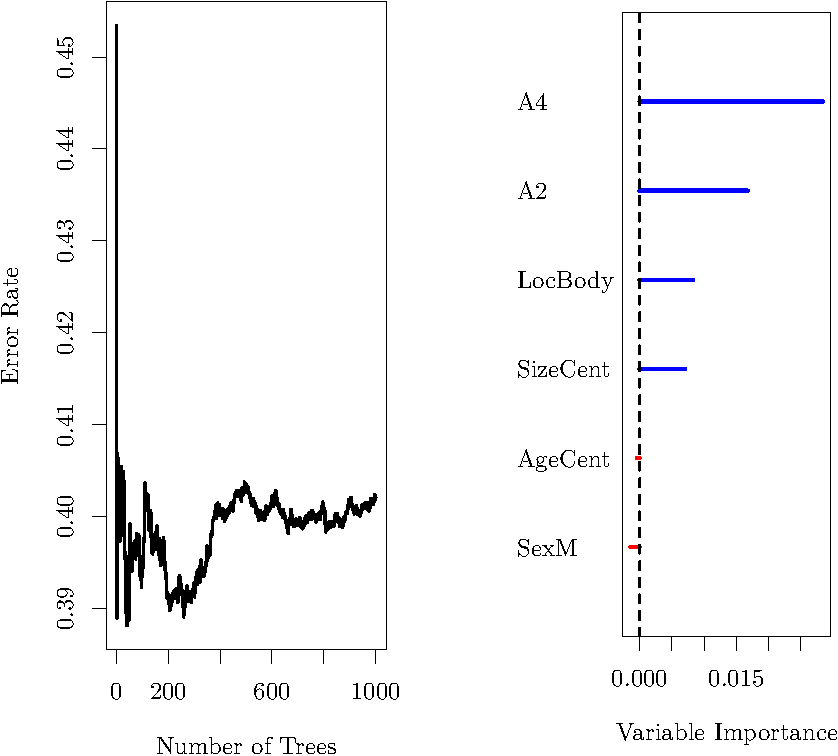
\includegraphics[width=\maxwidth]{figure/05-final-fits-rsf-1} 

}


\begin{kframe}\begin{verbatim}
## 
##            Importance   Relative Imp
## A4             0.0284         1.0000
## A2             0.0167         0.5887
## LocBody        0.0083         0.2920
## SizeCent       0.0071         0.2492
## AgeCent       -0.0004        -0.0149
## SexM          -0.0014        -0.0494
\end{verbatim}
\end{kframe}
\end{knitrout}

\begin{knitrout}
\definecolor{shadecolor}{rgb}{0.969, 0.969, 0.969}\color{fgcolor}\begin{kframe}
\begin{alltt}
\hlstd{fit.gg} \hlkwb{=} \hlkwd{flexsurvreg}\hlstd{(}\hlkwd{Surv}\hlstd{(Time, DSD)} \hlopt{~} \hlstd{SexM} \hlopt{+} \hlstd{LocBody} \hlopt{+} \hlstd{SizeCent} \hlopt{+} \hlstd{A2} \hlopt{+} \hlstd{A4,}
        \hlkwc{anc} \hlstd{=} \hlkwd{list}\hlstd{(}
                \hlkwc{sigma} \hlstd{=} \hlopt{~} \hlstd{SexM,}
                \hlkwc{Q} \hlstd{=} \hlopt{~} \hlstd{SexM),}
        \hlkwc{data} \hlstd{= data,} \hlkwc{dist} \hlstd{=} \hlstr{"gengamma"}\hlstd{)}

\hlstd{fit.gg2} \hlkwb{=} \hlkwd{flexsurvreg}\hlstd{(}\hlkwd{Surv}\hlstd{(Time, DSD)} \hlopt{~} \hlstd{SexM}\hlopt{+}\hlstd{AgeCent}\hlopt{+}\hlstd{LocBody}\hlopt{+}\hlstd{SizeCent}\hlopt{+}\hlstd{A2}\hlopt{+}\hlstd{A4}\hlopt{+}\hlstd{SizeCent}\hlopt{:}\hlstd{AgeCent}\hlopt{+}\hlstd{SexM}\hlopt{:}\hlstd{SizeCent,}
        \hlkwc{anc} \hlstd{=} \hlkwd{list}\hlstd{(}
                \hlkwc{sigma} \hlstd{=} \hlopt{~} \hlstd{SexM,}
                \hlkwc{Q} \hlstd{=} \hlopt{~} \hlstd{SexM),}
        \hlkwc{data} \hlstd{= data,} \hlkwc{dist} \hlstd{=} \hlstr{"gengamma"}\hlstd{)}

\hlstd{fit.gg}\hlopt{$}\hlstd{loglik}
\end{alltt}
\begin{verbatim}
## [1] -1325
\end{verbatim}
\begin{alltt}
\hlstd{fit.gg2}\hlopt{$}\hlstd{loglik}
\end{alltt}
\begin{verbatim}
## [1] -1321
\end{verbatim}
\begin{alltt}
\hlkwd{pchisq}\hlstd{(}\hlnum{2}\hlopt{*}\hlstd{(fit.gg2}\hlopt{$}\hlstd{loglik} \hlopt{-} \hlstd{fit.gg}\hlopt{$}\hlstd{loglik),} \hlnum{3}\hlstd{,} \hlkwc{lower.tail} \hlstd{=} \hlnum{FALSE}\hlstd{)}
\end{alltt}
\begin{verbatim}
## [1] 0.04837
\end{verbatim}
\begin{alltt}
\hlkwd{AIC}\hlstd{(fit.gg)}
\end{alltt}
\begin{verbatim}
## [1] 2669
\end{verbatim}
\begin{alltt}
\hlkwd{AIC}\hlstd{(fit.gg2)}
\end{alltt}
\begin{verbatim}
## [1] 2668
\end{verbatim}
\begin{alltt}
\hlstd{fit.gg}
\end{alltt}
\begin{verbatim}
## 
## Call:
## flexsurvreg(formula = Surv(Time, DSD) ~ SexM + LocBody + SizeCent +     A2 + A4, anc = list(sigma = ~SexM, Q = ~SexM), data = data,     dist = "gengamma")
## 
## Estimates: 
##                  data mean  est       L95%      U95%      se      
## mu                     NA    6.53611   6.19247   6.87976   0.17533
## sigma                  NA    0.78047   0.67245   0.90585   0.05932
## Q                      NA    0.11827  -0.49632   0.73287   0.31357
## SexMTRUE          0.51813    0.28181  -0.07256   0.63619   0.18081
## LocBodyTRUE       0.17098   -0.20952  -0.50577   0.08673   0.15115
## SizeCent          3.65285   -0.00879  -0.01600  -0.00158   0.00368
## A2TRUE            0.16580   -0.38962  -0.65941  -0.11983   0.13765
## A4TRUE            0.75130   -0.39725  -0.62687  -0.16763   0.11716
## sigma(SexMTRUE)   0.51813   -0.26267  -0.49374  -0.03159   0.11790
## Q(SexMTRUE)       0.51813    0.48452  -0.32987   1.29891   0.41551
##                  exp(est)  L95%      U95%    
## mu                     NA        NA        NA
## sigma                  NA        NA        NA
## Q                      NA        NA        NA
## SexMTRUE          1.32553   0.93001   1.88927
## LocBodyTRUE       0.81097   0.60304   1.09060
## SizeCent          0.99124   0.98412   0.99842
## A2TRUE            0.67731   0.51715   0.88707
## A4TRUE            0.67217   0.53426   0.84567
## sigma(SexMTRUE)   0.76900   0.61034   0.96890
## Q(SexMTRUE)       1.62340   0.71902   3.66531
## 
## N = 193,  Events: 184,  Censored: 9
## Total time at risk: 114833
## Log-likelihood = -1325, df = 10
## AIC = 2669
\end{verbatim}
\begin{alltt}
\hlstd{fit.gg2}
\end{alltt}
\begin{verbatim}
## 
## Call:
## flexsurvreg(formula = Surv(Time, DSD) ~ SexM + AgeCent + LocBody +     SizeCent + A2 + A4 + SizeCent:AgeCent + SexM:SizeCent, anc = list(sigma = ~SexM,     Q = ~SexM), data = data, dist = "gengamma")
## 
## Estimates: 
##                    data mean  est        L95%       U95%       se       
## mu                        NA   6.530218   6.184887   6.875549   0.176192
## sigma                     NA   0.771216   0.660311   0.900749   0.061092
## Q                         NA   0.228786  -0.410815   0.868387   0.326333
## SexMTRUE            0.518135   0.322116  -0.039753   0.683986   0.184631
## AgeCent            -1.067358   0.010352   0.000170   0.020534   0.005195
## LocBodyTRUE         0.170984  -0.271326  -0.558764   0.016113   0.146655
## SizeCent            3.652850  -0.004245  -0.015597   0.007107   0.005792
## A2TRUE              0.165803  -0.358631  -0.618603  -0.098660   0.132641
## A4TRUE              0.751295  -0.354054  -0.574822  -0.133287   0.112639
## AgeCent:SizeCent   -8.896373  -0.000855  -0.001550  -0.000160   0.000354
## SexMTRUE:SizeCent   1.772021  -0.006910  -0.020503   0.006684   0.006936
## sigma(SexMTRUE)     0.518135  -0.334045  -0.602093  -0.065998   0.136762
## Q(SexMTRUE)         0.518135   0.550014  -0.328860   1.428889   0.448414
##                    exp(est)   L95%       U95%     
## mu                        NA         NA         NA
## sigma                     NA         NA         NA
## Q                         NA         NA         NA
## SexMTRUE            1.380045   0.961027   1.981761
## AgeCent             1.010406   1.000170   1.020746
## LocBodyTRUE         0.762368   0.571915   1.016243
## SizeCent            0.995764   0.984524   1.007133
## A2TRUE              0.698632   0.538697   0.906051
## A4TRUE              0.701837   0.562805   0.875214
## AgeCent:SizeCent    0.999145   0.998452   0.999840
## SexMTRUE:SizeCent   0.993114   0.979706   1.006706
## sigma(SexMTRUE)     0.716021   0.547664   0.936133
## Q(SexMTRUE)         1.733278   0.719744   4.174059
## 
## N = 193,  Events: 184,  Censored: 9
## Total time at risk: 114833
## Log-likelihood = -1321, df = 13
## AIC = 2668
\end{verbatim}
\end{kframe}
\end{knitrout}

\section{Fit assessment}
Plot fit stratified by sex, separate curves for A2, A4 status, at median (approx.) Size.
\begin{knitrout}
\definecolor{shadecolor}{rgb}{0.969, 0.969, 0.969}\color{fgcolor}\begin{kframe}
\begin{alltt}
\hlstd{temp.grid} \hlkwb{=} \hlkwd{expand.grid}\hlstd{(}\hlkwc{A4} \hlstd{=} \hlkwd{c}\hlstd{(}\hlnum{FALSE}\hlstd{,} \hlnum{TRUE}\hlstd{),} \hlkwc{A2} \hlstd{=} \hlkwd{c}\hlstd{(}\hlnum{FALSE}\hlstd{,} \hlnum{TRUE}\hlstd{),} \hlkwc{SexM} \hlstd{=} \hlkwd{c}\hlstd{(}\hlnum{FALSE}\hlstd{,} \hlnum{TRUE}\hlstd{),} \hlkwc{SizeCent} \hlstd{=} \hlnum{0}\hlstd{,} \hlkwc{AgeCent} \hlstd{=} \hlnum{0}\hlstd{,} \hlkwc{SizePlus} \hlstd{=} \hlnum{0}\hlstd{,} \hlkwc{LocBody} \hlstd{=} \hlkwd{c}\hlstd{(}\hlnum{FALSE}\hlstd{,} \hlnum{TRUE}\hlstd{))}
\hlstd{temp.grid}\hlopt{$}\hlstd{ID} \hlkwb{=} \hlkwd{sprintf}\hlstd{(}\hlstr{"SexM=%s, A2=% -5s, A4=% -5s, LocBody=%s"}\hlstd{, temp.grid}\hlopt{$}\hlstd{SexM, temp.grid}\hlopt{$}\hlstd{A2, temp.grid}\hlopt{$}\hlstd{A4, temp.grid}\hlopt{$}\hlstd{LocBody)}
\hlstd{temp.preds} \hlkwb{=} \hlkwd{summary}\hlstd{(fit.gg,} \hlkwc{newdata} \hlstd{= temp.grid,} \hlkwc{type} \hlstd{=} \hlstr{"survival"}\hlstd{,} \hlkwc{t} \hlstd{=} \hlkwd{seq}\hlstd{(}\hlnum{0}\hlstd{,} \hlnum{365}\hlopt{*}\hlnum{5}\hlstd{,} \hlnum{30}\hlstd{))}
\hlstd{temp.preds2} \hlkwb{=} \hlkwd{do.call}\hlstd{(rbind, temp.preds)}
\hlstd{temp.preds2}\hlopt{$}\hlstd{group} \hlkwb{=} \hlkwd{rep}\hlstd{(}\hlkwd{gsub}\hlstd{(}\hlstr{".*ID="}\hlstd{,} \hlstr{""}\hlstd{,} \hlkwd{names}\hlstd{(temp.preds)),} \hlkwc{each} \hlstd{=} \hlkwd{nrow}\hlstd{(temp.preds[[}\hlnum{1}\hlstd{]]))}
\hlstd{temp.preds.cox} \hlkwb{=} \hlkwd{survfit}\hlstd{(fit.cph,} \hlkwc{newdata} \hlstd{= temp.grid)}
\hlstd{temp.preds.rsf} \hlkwb{=} \hlkwd{predict}\hlstd{(fit.rsf,} \hlkwc{newdata} \hlstd{= temp.grid)}

\hlstd{temp.survfit} \hlkwb{=} \hlkwd{survfit}\hlstd{(}\hlkwd{Surv}\hlstd{(Time, DSD)} \hlopt{~} \hlstd{SexM} \hlopt{+} \hlstd{A2} \hlopt{+} \hlstd{A4} \hlopt{+} \hlstd{LocBody, data)}
\hlstd{temp.data} \hlkwb{=} \hlkwd{data.frame}\hlstd{(}\hlkwc{time} \hlstd{= temp.survfit}\hlopt{$}\hlstd{time,} \hlkwc{surv} \hlstd{= temp.survfit}\hlopt{$}\hlstd{surv,} \hlkwc{upper} \hlstd{= temp.survfit}\hlopt{$}\hlstd{lower,} \hlkwc{lower} \hlstd{= temp.survfit}\hlopt{$}\hlstd{upper,} \hlkwc{group} \hlstd{=} \hlkwd{rep}\hlstd{(}\hlkwd{names}\hlstd{(temp.survfit}\hlopt{$}\hlstd{strata), temp.survfit}\hlopt{$}\hlstd{strata),} \hlkwc{model} \hlstd{=} \hlstr{"KM"}\hlstd{)}
\hlstd{temp.data} \hlkwb{=} \hlkwd{rbind}\hlstd{(temp.data,} \hlkwd{data.frame}\hlstd{(}\hlkwc{time} \hlstd{= temp.preds2}\hlopt{$}\hlstd{time,} \hlkwc{surv} \hlstd{= temp.preds2}\hlopt{$}\hlstd{est,} \hlkwc{upper} \hlstd{= temp.preds2}\hlopt{$}\hlstd{ucl,} \hlkwc{lower} \hlstd{= temp.preds2}\hlopt{$}\hlstd{lcl,} \hlkwc{group} \hlstd{= temp.preds2}\hlopt{$}\hlstd{group,} \hlkwc{model} \hlstd{=} \hlstr{"GG"}\hlstd{))}
\hlstd{temp.data} \hlkwb{=} \hlkwd{rbind}\hlstd{(temp.data,} \hlkwd{data.frame}\hlstd{(}\hlkwc{time} \hlstd{= temp.preds.cox}\hlopt{$}\hlstd{time,} \hlkwc{surv} \hlstd{= temp.preds.cox}\hlopt{$}\hlstd{surv,} \hlkwc{upper} \hlstd{= temp.preds.cox}\hlopt{$}\hlstd{upper,} \hlkwc{lower} \hlstd{= temp.preds.cox}\hlopt{$}\hlstd{lower,} \hlkwc{group} \hlstd{=} \hlkwd{rep}\hlstd{(temp.grid}\hlopt{$}\hlstd{ID, temp.preds.cox}\hlopt{$}\hlstd{strata),} \hlkwc{model} \hlstd{=} \hlstr{"CPH"}\hlstd{))}
\hlstd{temp.data} \hlkwb{=} \hlkwd{rbind}\hlstd{(temp.data,} \hlkwd{data.frame}\hlstd{(}\hlkwc{time} \hlstd{=} \hlkwd{rep}\hlstd{(temp.preds.rsf}\hlopt{$}\hlstd{time.interest,} \hlkwc{each} \hlstd{=} \hlkwd{nrow}\hlstd{(temp.preds.rsf}\hlopt{$}\hlstd{survival)),} \hlkwc{surv} \hlstd{=} \hlkwd{as.vector}\hlstd{(temp.preds.rsf}\hlopt{$}\hlstd{survival),} \hlkwc{upper} \hlstd{=} \hlnum{NA}\hlstd{,} \hlkwc{lower} \hlstd{=} \hlnum{NA}\hlstd{,} \hlkwc{group} \hlstd{=} \hlkwd{rep}\hlstd{(temp.grid}\hlopt{$}\hlstd{ID,} \hlkwd{length}\hlstd{(temp.preds.rsf}\hlopt{$}\hlstd{time.interest)),} \hlkwc{model} \hlstd{=} \hlstr{"RSF"}\hlstd{))}

\hlstd{temp.data}\hlopt{$}\hlstd{Sex} \hlkwb{=} \hlkwd{c}\hlstd{(}\hlstr{"Male"}\hlstd{,} \hlstr{"Female"}\hlstd{)[}\hlkwd{grepl}\hlstd{(}\hlstr{"SexM=FALSE"}\hlstd{, temp.data}\hlopt{$}\hlstd{group)}\hlopt{+}\hlnum{1}\hlstd{]}
\hlstd{temp.data}\hlopt{$}\hlstd{A2} \hlkwb{=} \hlkwd{c}\hlstd{(}\hlstr{"A2-"}\hlstd{,} \hlstr{"A2+"}\hlstd{)[}\hlkwd{grepl}\hlstd{(}\hlstr{"A2=TRUE"}\hlstd{, temp.data}\hlopt{$}\hlstd{group)}\hlopt{+}\hlnum{1}\hlstd{]}
\hlstd{temp.data}\hlopt{$}\hlstd{A4} \hlkwb{=} \hlkwd{c}\hlstd{(}\hlstr{"A4-"}\hlstd{,} \hlstr{"A4+"}\hlstd{)[}\hlkwd{grepl}\hlstd{(}\hlstr{"A4=TRUE"}\hlstd{, temp.data}\hlopt{$}\hlstd{group)}\hlopt{+}\hlnum{1}\hlstd{]}
\hlstd{temp.data}\hlopt{$}\hlstd{Location} \hlkwb{=} \hlkwd{c}\hlstd{(}\hlstr{"Head"}\hlstd{,} \hlstr{"Body"}\hlstd{)[}\hlkwd{grepl}\hlstd{(}\hlstr{"LocBody=TRUE"}\hlstd{, temp.data}\hlopt{$}\hlstd{group)}\hlopt{+}\hlnum{1}\hlstd{]}

\hlstd{temp.data}\hlopt{$}\hlstd{lower[temp.data}\hlopt{$}\hlstd{model} \hlopt{!=} \hlstr{"KM"}\hlstd{]} \hlkwb{=} \hlnum{NA}
\hlstd{temp.data}\hlopt{$}\hlstd{upper[temp.data}\hlopt{$}\hlstd{model} \hlopt{!=} \hlstr{"KM"}\hlstd{]} \hlkwb{=} \hlnum{NA}
\hlkwd{ggplot}\hlstd{(temp.data,} \hlkwd{aes}\hlstd{(}\hlkwc{x} \hlstd{=} \hlkwd{log}\hlstd{(time),} \hlkwc{y} \hlstd{=} \hlkwd{log}\hlstd{(}\hlopt{-}\hlkwd{log}\hlstd{(surv)),} \hlkwc{ymin} \hlstd{=} \hlkwd{log}\hlstd{(}\hlopt{-}\hlkwd{log}\hlstd{(lower)),} \hlkwc{ymax} \hlstd{=} \hlkwd{log}\hlstd{(}\hlopt{-}\hlkwd{log}\hlstd{(upper)),} \hlkwc{colour} \hlstd{= model,} \hlkwc{fill} \hlstd{= model))} \hlopt{+}
        \hlkwd{geom_ribbon}\hlstd{(}\hlkwc{alpha} \hlstd{=} \hlnum{0.25}\hlstd{,} \hlkwc{colour} \hlstd{=} \hlnum{NA}\hlstd{)} \hlopt{+}
        \hlkwd{geom_line}\hlstd{()} \hlopt{+}
        \hlkwd{xlim}\hlstd{(}\hlnum{4}\hlstd{,} \hlnum{7}\hlstd{)} \hlopt{+} \hlkwd{ylim}\hlstd{(}\hlopt{-}\hlnum{4}\hlstd{,} \hlnum{2}\hlstd{)} \hlopt{+}
        \hlkwd{facet_grid}\hlstd{(A2} \hlopt{~} \hlstd{A4} \hlopt{~} \hlstd{Sex} \hlopt{~} \hlstd{Location)}
\end{alltt}


{\ttfamily\noindent\color{warningcolor}{\#\# Warning: Removed 64 rows containing missing values (geom\_path).}}

{\ttfamily\noindent\color{warningcolor}{\#\# Warning: Removed 70 rows containing missing values (geom\_path).}}

{\ttfamily\noindent\color{warningcolor}{\#\# Warning: Removed 59 rows containing missing values (geom\_path).}}

{\ttfamily\noindent\color{warningcolor}{\#\# Warning: Removed 69 rows containing missing values (geom\_path).}}

{\ttfamily\noindent\color{warningcolor}{\#\# Warning: Removed 60 rows containing missing values (geom\_path).}}

{\ttfamily\noindent\color{warningcolor}{\#\# Warning: Removed 70 rows containing missing values (geom\_path).}}

{\ttfamily\noindent\color{warningcolor}{\#\# Warning: Removed 57 rows containing missing values (geom\_path).}}

{\ttfamily\noindent\color{warningcolor}{\#\# Warning: Removed 66 rows containing missing values (geom\_path).}}

{\ttfamily\noindent\color{warningcolor}{\#\# Warning: Removed 58 rows containing missing values (geom\_path).}}

{\ttfamily\noindent\color{warningcolor}{\#\# Warning: Removed 59 rows containing missing values (geom\_path).}}

{\ttfamily\noindent\color{warningcolor}{\#\# Warning: Removed 56 rows containing missing values (geom\_path).}}

{\ttfamily\noindent\color{warningcolor}{\#\# Warning: Removed 56 rows containing missing values (geom\_path).}}

{\ttfamily\noindent\color{warningcolor}{\#\# Warning: Removed 57 rows containing missing values (geom\_path).}}

{\ttfamily\noindent\color{warningcolor}{\#\# Warning: Removed 58 rows containing missing values (geom\_path).}}

{\ttfamily\noindent\color{warningcolor}{\#\# Warning: Removed 57 rows containing missing values (geom\_path).}}

{\ttfamily\noindent\color{warningcolor}{\#\# Warning: Removed 56 rows containing missing values (geom\_path).}}\end{kframe}

{\centering 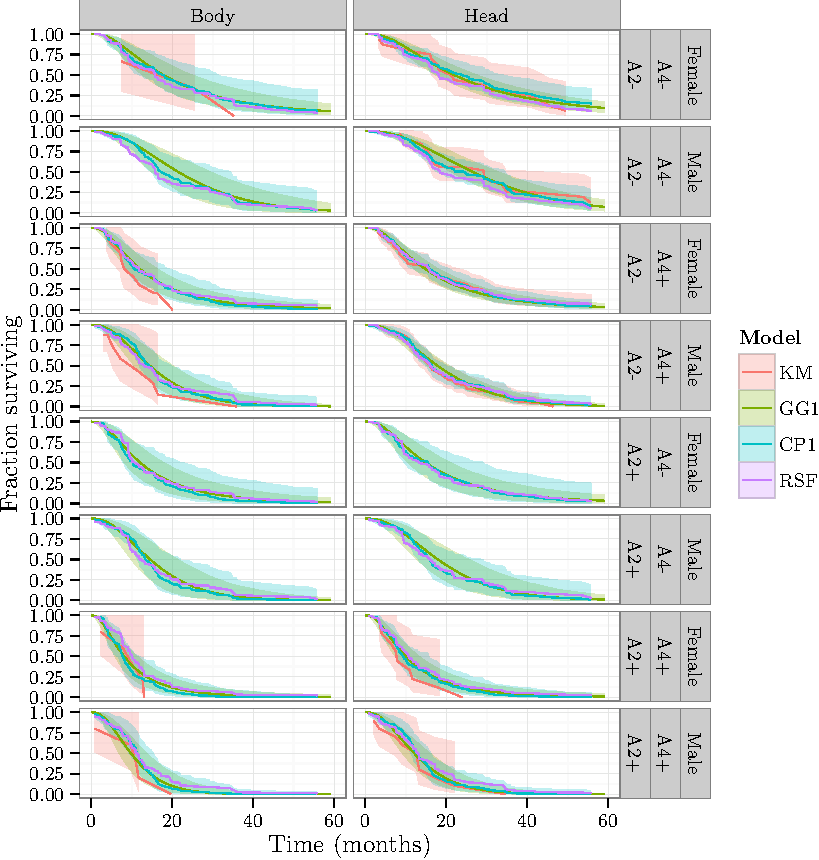
\includegraphics[width=\maxwidth]{figure/05-final-fit-assessment-1} 

}


\begin{kframe}\begin{alltt}
\hlkwd{ggplot}\hlstd{(temp.data,} \hlkwd{aes}\hlstd{(}\hlkwc{x} \hlstd{= time,} \hlkwc{y} \hlstd{= surv,} \hlkwc{ymin} \hlstd{= lower,} \hlkwc{ymax} \hlstd{= upper,} \hlkwc{colour} \hlstd{= model,} \hlkwc{fill} \hlstd{= model))} \hlopt{+}
        \hlkwd{geom_ribbon}\hlstd{(}\hlkwc{alpha} \hlstd{=} \hlnum{0.25}\hlstd{,} \hlkwc{colour} \hlstd{=} \hlnum{NA}\hlstd{)} \hlopt{+}
        \hlkwd{geom_line}\hlstd{()} \hlopt{+} \hlkwd{xlim}\hlstd{(}\hlnum{0}\hlstd{,} \hlnum{2000}\hlstd{)} \hlopt{+} \hlkwd{ylim}\hlstd{(}\hlnum{0}\hlstd{,} \hlnum{1}\hlstd{)} \hlopt{+}
        \hlkwd{facet_grid}\hlstd{(A2} \hlopt{~} \hlstd{A4} \hlopt{~} \hlstd{Sex} \hlopt{~} \hlstd{Location)}
\end{alltt}


{\ttfamily\noindent\color{warningcolor}{\#\# Warning: Removed 4 rows containing missing values (geom\_path).}}

{\ttfamily\noindent\color{warningcolor}{\#\# Warning: Removed 5 rows containing missing values (geom\_path).}}

{\ttfamily\noindent\color{warningcolor}{\#\# Warning: Removed 3 rows containing missing values (geom\_path).}}

{\ttfamily\noindent\color{warningcolor}{\#\# Warning: Removed 4 rows containing missing values (geom\_path).}}

{\ttfamily\noindent\color{warningcolor}{\#\# Warning: Removed 4 rows containing missing values (geom\_path).}}

{\ttfamily\noindent\color{warningcolor}{\#\# Warning: Removed 5 rows containing missing values (geom\_path).}}

{\ttfamily\noindent\color{warningcolor}{\#\# Warning: Removed 3 rows containing missing values (geom\_path).}}

{\ttfamily\noindent\color{warningcolor}{\#\# Warning: Removed 3 rows containing missing values (geom\_path).}}

{\ttfamily\noindent\color{warningcolor}{\#\# Warning: Removed 4 rows containing missing values (geom\_path).}}

{\ttfamily\noindent\color{warningcolor}{\#\# Warning: Removed 4 rows containing missing values (geom\_path).}}

{\ttfamily\noindent\color{warningcolor}{\#\# Warning: Removed 3 rows containing missing values (geom\_path).}}

{\ttfamily\noindent\color{warningcolor}{\#\# Warning: Removed 3 rows containing missing values (geom\_path).}}

{\ttfamily\noindent\color{warningcolor}{\#\# Warning: Removed 4 rows containing missing values (geom\_path).}}

{\ttfamily\noindent\color{warningcolor}{\#\# Warning: Removed 4 rows containing missing values (geom\_path).}}

{\ttfamily\noindent\color{warningcolor}{\#\# Warning: Removed 3 rows containing missing values (geom\_path).}}

{\ttfamily\noindent\color{warningcolor}{\#\# Warning: Removed 3 rows containing missing values (geom\_path).}}\end{kframe}

{\centering 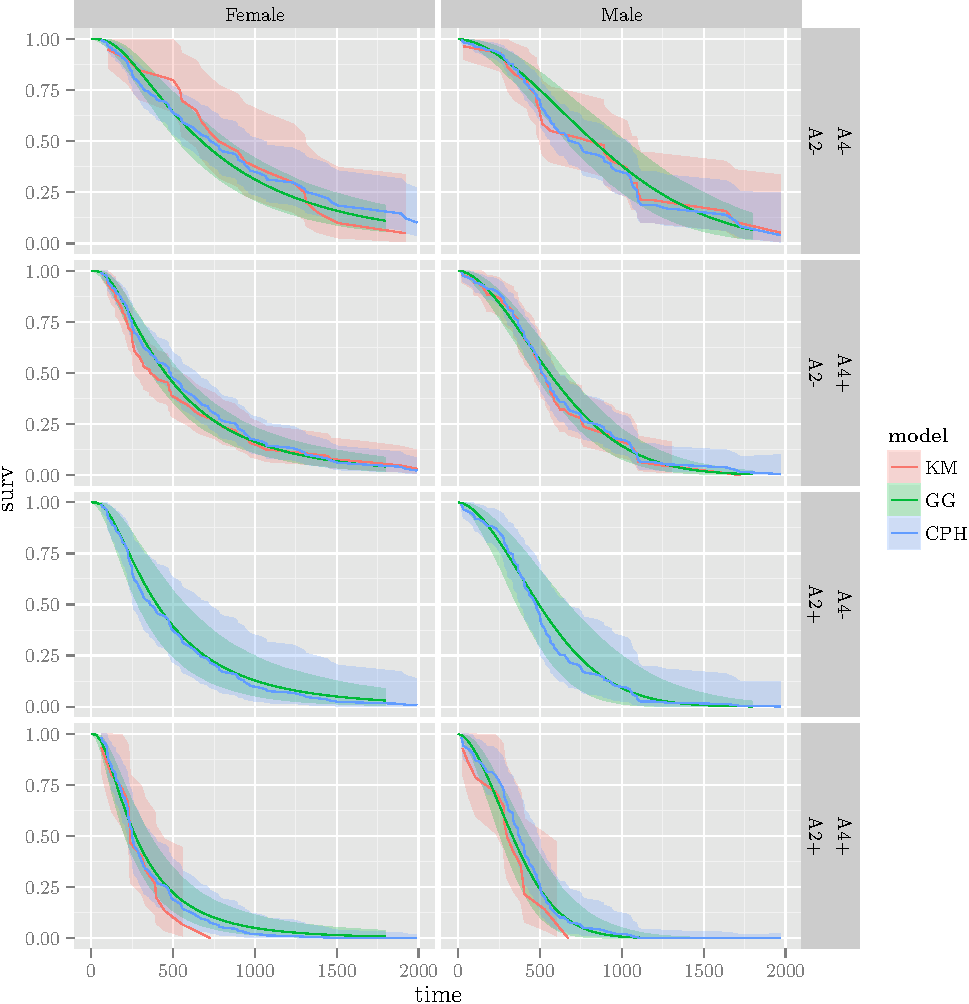
\includegraphics[width=\maxwidth]{figure/05-final-fit-assessment-2} 

}


\begin{kframe}\begin{alltt}
\hlstd{temp.grid} \hlkwb{=} \hlkwd{expand.grid}\hlstd{(}\hlkwc{A4} \hlstd{=} \hlkwd{c}\hlstd{(}\hlnum{FALSE}\hlstd{,} \hlnum{TRUE}\hlstd{),} \hlkwc{A2} \hlstd{=} \hlkwd{c}\hlstd{(}\hlnum{FALSE}\hlstd{,} \hlnum{TRUE}\hlstd{),} \hlkwc{SexM} \hlstd{=} \hlkwd{c}\hlstd{(}\hlnum{FALSE}\hlstd{,} \hlnum{TRUE}\hlstd{),} \hlkwc{SizeCent} \hlstd{=} \hlnum{0}\hlstd{,} \hlkwc{AgeCent} \hlstd{=} \hlnum{0}\hlstd{,} \hlkwc{SizePlus} \hlstd{=} \hlnum{0}\hlstd{,} \hlkwc{LocBody} \hlstd{=} \hlnum{FALSE}\hlstd{)}
\hlstd{temp.grid}\hlopt{$}\hlstd{ID} \hlkwb{=} \hlkwd{sprintf}\hlstd{(}\hlstr{"SexM=%s, A2=% -5s, A4=% -5s, LocBody=%s"}\hlstd{, temp.grid}\hlopt{$}\hlstd{SexM, temp.grid}\hlopt{$}\hlstd{A2, temp.grid}\hlopt{$}\hlstd{A4, temp.grid}\hlopt{$}\hlstd{LocBody)}
\hlstd{temp.preds} \hlkwb{=} \hlkwd{summary}\hlstd{(fit.gg,} \hlkwc{newdata} \hlstd{= temp.grid,} \hlkwc{type} \hlstd{=} \hlstr{"survival"}\hlstd{,} \hlkwc{t} \hlstd{=} \hlkwd{seq}\hlstd{(}\hlnum{0}\hlstd{,} \hlnum{365}\hlopt{*}\hlnum{5}\hlstd{,} \hlnum{30}\hlstd{))}
\hlstd{temp.preds2} \hlkwb{=} \hlkwd{do.call}\hlstd{(rbind, temp.preds)}
\hlstd{temp.preds2}\hlopt{$}\hlstd{group} \hlkwb{=} \hlkwd{rep}\hlstd{(}\hlkwd{gsub}\hlstd{(}\hlstr{".*ID="}\hlstd{,} \hlstr{""}\hlstd{,} \hlkwd{names}\hlstd{(temp.preds)),} \hlkwc{each} \hlstd{=} \hlkwd{nrow}\hlstd{(temp.preds[[}\hlnum{1}\hlstd{]]))}
\hlstd{temp.preds.cox} \hlkwb{=} \hlkwd{survfit}\hlstd{(fit.cph,} \hlkwc{newdata} \hlstd{= temp.grid)}
\hlstd{temp.preds.rsf} \hlkwb{=} \hlkwd{predict}\hlstd{(fit.rsf,} \hlkwc{newdata} \hlstd{= temp.grid)}

\hlstd{temp.survfit} \hlkwb{=} \hlkwd{survfit}\hlstd{(}\hlkwd{Surv}\hlstd{(Time, DSD)} \hlopt{~} \hlstd{SexM} \hlopt{+} \hlstd{A2} \hlopt{+} \hlstd{A4, data)}
\hlstd{temp.data} \hlkwb{=} \hlkwd{data.frame}\hlstd{(}\hlkwc{time} \hlstd{= temp.survfit}\hlopt{$}\hlstd{time,} \hlkwc{surv} \hlstd{= temp.survfit}\hlopt{$}\hlstd{surv,} \hlkwc{upper} \hlstd{= temp.survfit}\hlopt{$}\hlstd{lower,} \hlkwc{lower} \hlstd{= temp.survfit}\hlopt{$}\hlstd{upper,} \hlkwc{group} \hlstd{=} \hlkwd{rep}\hlstd{(}\hlkwd{names}\hlstd{(temp.survfit}\hlopt{$}\hlstd{strata), temp.survfit}\hlopt{$}\hlstd{strata),} \hlkwc{model} \hlstd{=} \hlstr{"KM"}\hlstd{)}
\hlstd{temp.data} \hlkwb{=} \hlkwd{rbind}\hlstd{(temp.data,} \hlkwd{data.frame}\hlstd{(}\hlkwc{time} \hlstd{= temp.preds2}\hlopt{$}\hlstd{time,} \hlkwc{surv} \hlstd{= temp.preds2}\hlopt{$}\hlstd{est,} \hlkwc{upper} \hlstd{= temp.preds2}\hlopt{$}\hlstd{ucl,} \hlkwc{lower} \hlstd{= temp.preds2}\hlopt{$}\hlstd{lcl,} \hlkwc{group} \hlstd{= temp.preds2}\hlopt{$}\hlstd{group,} \hlkwc{model} \hlstd{=} \hlstr{"GG"}\hlstd{))}
\hlstd{temp.data} \hlkwb{=} \hlkwd{rbind}\hlstd{(temp.data,} \hlkwd{data.frame}\hlstd{(}\hlkwc{time} \hlstd{= temp.preds.cox}\hlopt{$}\hlstd{time,} \hlkwc{surv} \hlstd{= temp.preds.cox}\hlopt{$}\hlstd{surv,} \hlkwc{upper} \hlstd{= temp.preds.cox}\hlopt{$}\hlstd{upper,} \hlkwc{lower} \hlstd{= temp.preds.cox}\hlopt{$}\hlstd{lower,} \hlkwc{group} \hlstd{=} \hlkwd{rep}\hlstd{(temp.grid}\hlopt{$}\hlstd{ID, temp.preds.cox}\hlopt{$}\hlstd{strata),} \hlkwc{model} \hlstd{=} \hlstr{"CPH"}\hlstd{))}
\hlstd{temp.data} \hlkwb{=} \hlkwd{rbind}\hlstd{(temp.data,} \hlkwd{data.frame}\hlstd{(}\hlkwc{time} \hlstd{=} \hlkwd{rep}\hlstd{(temp.preds.rsf}\hlopt{$}\hlstd{time.interest,} \hlkwc{each} \hlstd{=} \hlkwd{nrow}\hlstd{(temp.preds.rsf}\hlopt{$}\hlstd{survival)),} \hlkwc{surv} \hlstd{=} \hlkwd{as.vector}\hlstd{(temp.preds.rsf}\hlopt{$}\hlstd{survival),} \hlkwc{upper} \hlstd{=} \hlnum{NA}\hlstd{,} \hlkwc{lower} \hlstd{=} \hlnum{NA}\hlstd{,} \hlkwc{group} \hlstd{=} \hlkwd{rep}\hlstd{(temp.grid}\hlopt{$}\hlstd{ID,} \hlkwd{length}\hlstd{(temp.preds.rsf}\hlopt{$}\hlstd{time.interest)),} \hlkwc{model} \hlstd{=} \hlstr{"RSF"}\hlstd{))}

\hlstd{temp.data}\hlopt{$}\hlstd{Sex} \hlkwb{=} \hlkwd{c}\hlstd{(}\hlstr{"Male"}\hlstd{,} \hlstr{"Female"}\hlstd{)[}\hlkwd{grepl}\hlstd{(}\hlstr{"SexM=FALSE"}\hlstd{, temp.data}\hlopt{$}\hlstd{group)}\hlopt{+}\hlnum{1}\hlstd{]}
\hlstd{temp.data}\hlopt{$}\hlstd{A2} \hlkwb{=} \hlkwd{c}\hlstd{(}\hlstr{"A2-"}\hlstd{,} \hlstr{"A2+"}\hlstd{)[}\hlkwd{grepl}\hlstd{(}\hlstr{"A2=TRUE"}\hlstd{, temp.data}\hlopt{$}\hlstd{group)}\hlopt{+}\hlnum{1}\hlstd{]}
\hlstd{temp.data}\hlopt{$}\hlstd{A4} \hlkwb{=} \hlkwd{c}\hlstd{(}\hlstr{"A4-"}\hlstd{,} \hlstr{"A4+"}\hlstd{)[}\hlkwd{grepl}\hlstd{(}\hlstr{"A4=TRUE"}\hlstd{, temp.data}\hlopt{$}\hlstd{group)}\hlopt{+}\hlnum{1}\hlstd{]}

\hlstd{temp.data}\hlopt{$}\hlstd{lower[temp.data}\hlopt{$}\hlstd{model} \hlopt{!=} \hlstr{"KM"}\hlstd{]} \hlkwb{=} \hlnum{NA}
\hlstd{temp.data}\hlopt{$}\hlstd{upper[temp.data}\hlopt{$}\hlstd{model} \hlopt{!=} \hlstr{"KM"}\hlstd{]} \hlkwb{=} \hlnum{NA}
\hlkwd{ggplot}\hlstd{(temp.data,} \hlkwd{aes}\hlstd{(}\hlkwc{x} \hlstd{=} \hlkwd{log}\hlstd{(time),} \hlkwc{y} \hlstd{=} \hlkwd{log}\hlstd{(}\hlopt{-}\hlkwd{log}\hlstd{(surv)),} \hlkwc{ymin} \hlstd{=} \hlkwd{log}\hlstd{(}\hlopt{-}\hlkwd{log}\hlstd{(lower)),} \hlkwc{ymax} \hlstd{=} \hlkwd{log}\hlstd{(}\hlopt{-}\hlkwd{log}\hlstd{(upper)),} \hlkwc{colour} \hlstd{= model,} \hlkwc{fill} \hlstd{= model))} \hlopt{+}
        \hlkwd{geom_ribbon}\hlstd{(}\hlkwc{alpha} \hlstd{=} \hlnum{0.25}\hlstd{,} \hlkwc{colour} \hlstd{=} \hlnum{NA}\hlstd{)} \hlopt{+}
        \hlkwd{geom_line}\hlstd{()} \hlopt{+}
        \hlkwd{xlim}\hlstd{(}\hlnum{4}\hlstd{,} \hlnum{7}\hlstd{)} \hlopt{+} \hlkwd{ylim}\hlstd{(}\hlopt{-}\hlnum{4}\hlstd{,} \hlnum{2}\hlstd{)} \hlopt{+}
        \hlkwd{facet_grid}\hlstd{(A2} \hlopt{~} \hlstd{A4} \hlopt{~} \hlstd{Sex)}
\end{alltt}


{\ttfamily\noindent\color{warningcolor}{\#\# Warning: Removed 70 rows containing missing values (geom\_path).}}

{\ttfamily\noindent\color{warningcolor}{\#\# Warning: Removed 69 rows containing missing values (geom\_path).}}

{\ttfamily\noindent\color{warningcolor}{\#\# Warning: Removed 71 rows containing missing values (geom\_path).}}

{\ttfamily\noindent\color{warningcolor}{\#\# Warning: Removed 67 rows containing missing values (geom\_path).}}

{\ttfamily\noindent\color{warningcolor}{\#\# Warning: Removed 59 rows containing missing values (geom\_path).}}

{\ttfamily\noindent\color{warningcolor}{\#\# Warning: Removed 56 rows containing missing values (geom\_path).}}

{\ttfamily\noindent\color{warningcolor}{\#\# Warning: Removed 58 rows containing missing values (geom\_path).}}

{\ttfamily\noindent\color{warningcolor}{\#\# Warning: Removed 57 rows containing missing values (geom\_path).}}\end{kframe}

{\centering 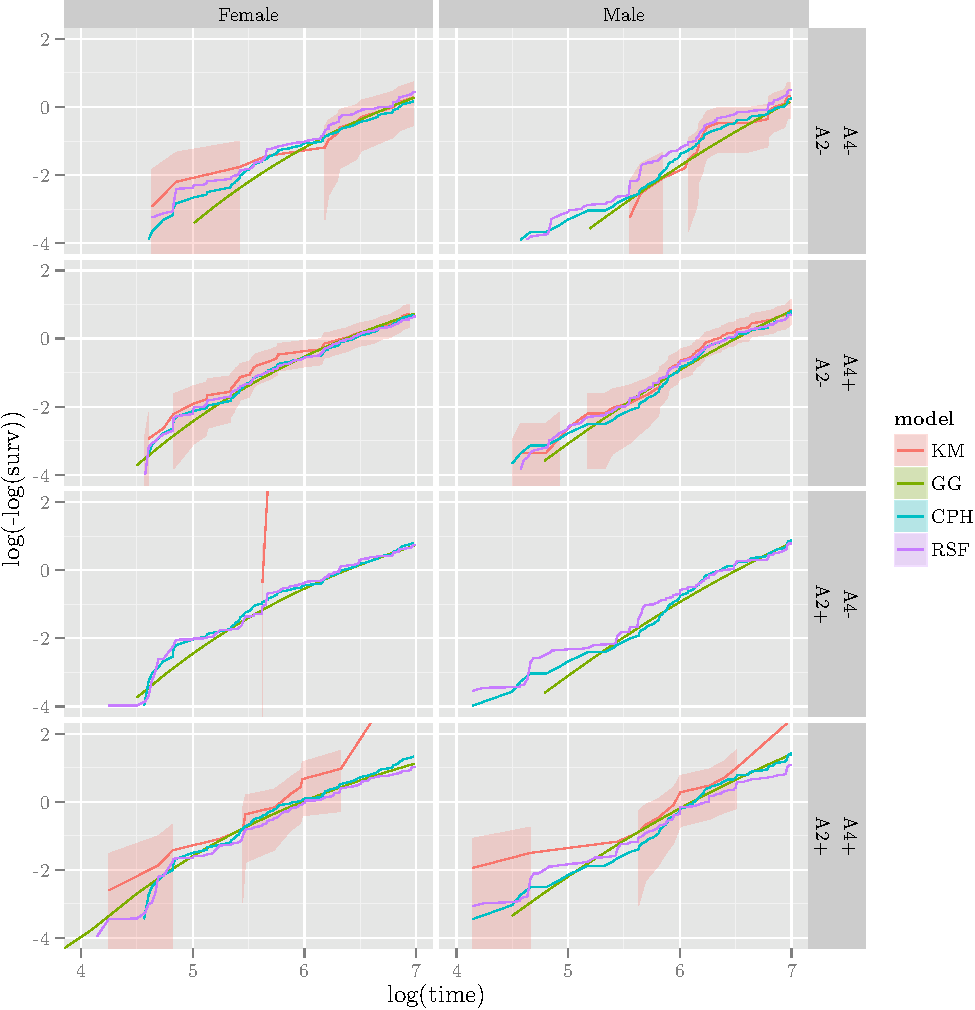
\includegraphics[width=\maxwidth]{figure/05-final-fit-assessment-3} 

}


\begin{kframe}\begin{alltt}
\hlkwd{ggplot}\hlstd{(temp.data,} \hlkwd{aes}\hlstd{(}\hlkwc{x} \hlstd{= time,} \hlkwc{y} \hlstd{= surv,} \hlkwc{ymin} \hlstd{= lower,} \hlkwc{ymax} \hlstd{= upper,} \hlkwc{colour} \hlstd{= model,} \hlkwc{fill} \hlstd{= model))} \hlopt{+}
        \hlkwd{geom_ribbon}\hlstd{(}\hlkwc{alpha} \hlstd{=} \hlnum{0.25}\hlstd{,} \hlkwc{colour} \hlstd{=} \hlnum{NA}\hlstd{)} \hlopt{+}
        \hlkwd{geom_line}\hlstd{()} \hlopt{+} \hlkwd{xlim}\hlstd{(}\hlnum{0}\hlstd{,} \hlnum{2000}\hlstd{)} \hlopt{+} \hlkwd{ylim}\hlstd{(}\hlnum{0}\hlstd{,} \hlnum{1}\hlstd{)} \hlopt{+}
        \hlkwd{facet_grid}\hlstd{(A2} \hlopt{~} \hlstd{A4} \hlopt{~} \hlstd{Sex)}
\end{alltt}


{\ttfamily\noindent\color{warningcolor}{\#\# Warning: Removed 5 rows containing missing values (geom\_path).}}

{\ttfamily\noindent\color{warningcolor}{\#\# Warning: Removed 4 rows containing missing values (geom\_path).}}

{\ttfamily\noindent\color{warningcolor}{\#\# Warning: Removed 5 rows containing missing values (geom\_path).}}

{\ttfamily\noindent\color{warningcolor}{\#\# Warning: Removed 3 rows containing missing values (geom\_path).}}

{\ttfamily\noindent\color{warningcolor}{\#\# Warning: Removed 4 rows containing missing values (geom\_path).}}

{\ttfamily\noindent\color{warningcolor}{\#\# Warning: Removed 3 rows containing missing values (geom\_path).}}

{\ttfamily\noindent\color{warningcolor}{\#\# Warning: Removed 4 rows containing missing values (geom\_path).}}

{\ttfamily\noindent\color{warningcolor}{\#\# Warning: Removed 3 rows containing missing values (geom\_path).}}\end{kframe}

{\centering 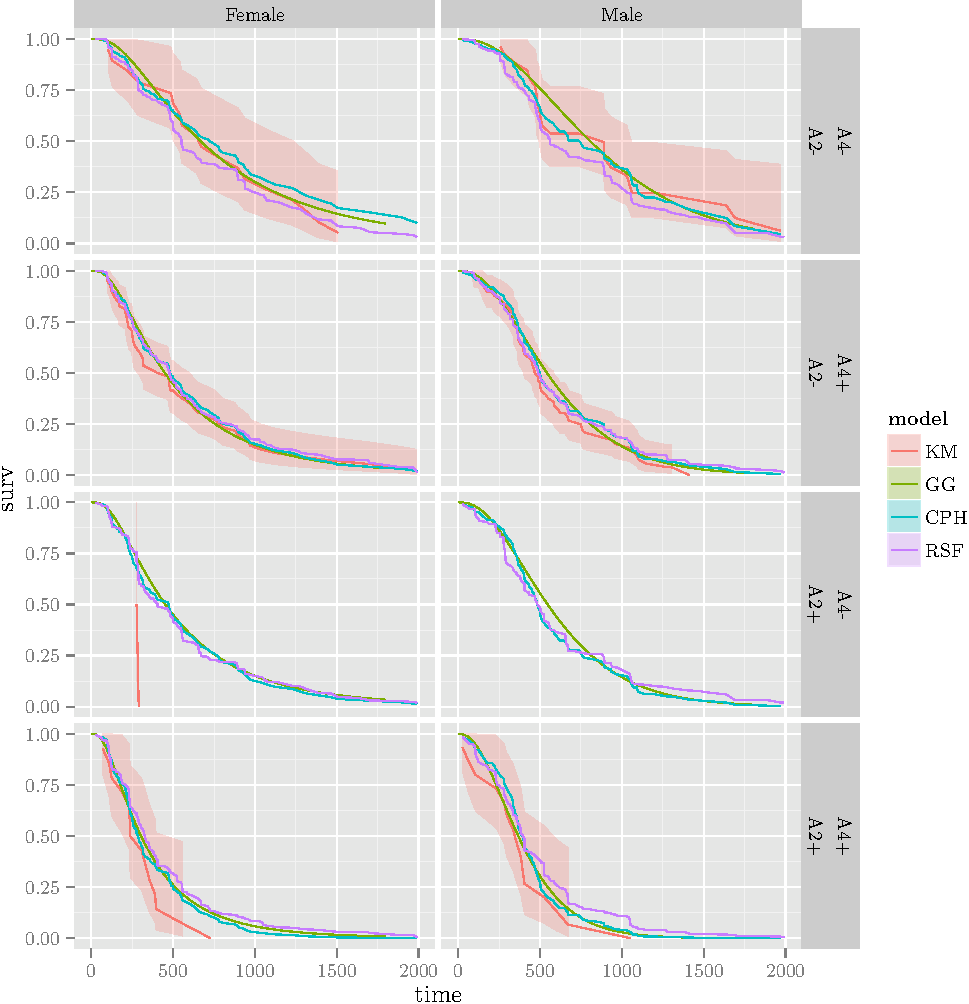
\includegraphics[width=\maxwidth]{figure/05-final-fit-assessment-4} 

}



\end{knitrout}


\section{Model selection}
It looks like that's as far as we can go with tweaking the fits.  Time to put the different models against each other on the holdout data, and choose a winner.

DIY IBS, wooo.
\begin{knitrout}
\definecolor{shadecolor}{rgb}{0.969, 0.969, 0.969}\color{fgcolor}\begin{kframe}
\begin{alltt}
\hlstd{calcIBS} \hlkwb{=} \hlkwa{function}\hlstd{(}\hlkwc{surv}\hlstd{,} \hlkwc{pred}\hlstd{,} \hlkwc{pred_times}\hlstd{,} \hlkwc{max_time}\hlstd{,} \hlkwc{min_time} \hlstd{=} \hlnum{0}\hlstd{)}
\hlstd{\{}
        \hlkwd{stopifnot}\hlstd{(}\hlkwd{nrow}\hlstd{(surv)} \hlopt{==} \hlkwd{nrow}\hlstd{(pred)} \hlopt{&&} \hlkwd{length}\hlstd{(pred_times)} \hlopt{==} \hlkwd{ncol}\hlstd{(pred))}

        \hlstd{n} \hlkwb{=} \hlkwd{nrow}\hlstd{(surv)}
        \hlstd{marg_survfit} \hlkwb{=} \hlkwd{survfit}\hlstd{(surv} \hlopt{~} \hlnum{1}\hlstd{)}
        \hlstd{marg_censfit} \hlkwb{=} \hlkwd{survfit}\hlstd{(}\hlkwd{Surv}\hlstd{(surv[,}\hlnum{1}\hlstd{],} \hlopt{!}\hlstd{surv[,}\hlnum{2}\hlstd{])} \hlopt{~} \hlnum{1}\hlstd{)}
        \hlstd{marg_surv_func} \hlkwb{=} \hlkwd{approxfun}\hlstd{(marg_survfit}\hlopt{$}\hlstd{time, marg_survfit}\hlopt{$}\hlstd{surv,} \hlkwc{method} \hlstd{=} \hlstr{"constant"}\hlstd{,} \hlkwc{yleft} \hlstd{=} \hlnum{1}\hlstd{,} \hlkwc{yright} \hlstd{=} \hlnum{0}\hlstd{,} \hlkwc{rule} \hlstd{=} \hlnum{2}\hlopt{:}\hlnum{1}\hlstd{,} \hlkwc{f} \hlstd{=} \hlnum{0}\hlstd{)}
        \hlstd{marg_cens_func} \hlkwb{=} \hlkwd{approxfun}\hlstd{(marg_censfit}\hlopt{$}\hlstd{time, marg_censfit}\hlopt{$}\hlstd{surv,} \hlkwc{method} \hlstd{=} \hlstr{"constant"}\hlstd{,} \hlkwc{yleft} \hlstd{=} \hlnum{1}\hlstd{,} \hlkwc{yright} \hlstd{=} \hlnum{0}\hlstd{,} \hlkwc{rule} \hlstd{=} \hlnum{2}\hlopt{:}\hlnum{1}\hlstd{,} \hlkwc{f} \hlstd{=} \hlnum{0}\hlstd{)}

        \hlstd{pred_funcs} \hlkwb{=} \hlkwd{apply}\hlstd{(pred,} \hlnum{1}\hlstd{,} \hlkwa{function}\hlstd{(}\hlkwc{pat_preds}\hlstd{)} \hlkwd{approxfun}\hlstd{(pred_times, pat_preds,} \hlkwc{yleft} \hlstd{=} \hlnum{1}\hlstd{,} \hlkwc{yright} \hlstd{=} \hlkwd{min}\hlstd{(pat_preds),} \hlkwc{rule} \hlstd{=} \hlnum{2}\hlstd{))}

        \hlstd{indiv_patient_bsc} \hlkwb{=} \hlkwa{function}\hlstd{(}\hlkwc{pat_i}\hlstd{,} \hlkwc{tstars}\hlstd{)}
        \hlstd{\{}
                \hlstd{observed_time} \hlkwb{=} \hlstd{surv[pat_i,} \hlnum{1}\hlstd{]}
                \hlstd{observed_event} \hlkwb{=} \hlstd{surv[pat_i,} \hlnum{2}\hlstd{]}
                \hlstd{pred_func} \hlkwb{=} \hlstd{pred_funcs[[pat_i]]}
                \hlstd{category} \hlkwb{=} \hlnum{1}\hlopt{*}\hlstd{(observed_time} \hlopt{<=} \hlstd{tstars} \hlopt{&} \hlstd{observed_event)} \hlopt{+} \hlnum{2}\hlopt{*}\hlstd{(observed_time} \hlopt{>} \hlstd{tstars)} \hlopt{+} \hlnum{3}\hlopt{*}\hlstd{(observed_time} \hlopt{<=} \hlstd{tstars} \hlopt{& !}\hlstd{observed_event)}
                \hlstd{bsc} \hlkwb{=} \hlkwd{rep}\hlstd{(}\hlnum{NA}\hlstd{,} \hlkwd{length}\hlstd{(tstars))}
                \hlstd{bsc[category} \hlopt{==} \hlnum{1}\hlstd{]} \hlkwb{=} \hlkwd{pred_func}\hlstd{(tstars[category} \hlopt{==} \hlnum{1}\hlstd{])}\hlopt{^}\hlnum{2} \hlopt{/} \hlkwd{marg_cens_func}\hlstd{(observed_time)}
                \hlstd{bsc[category} \hlopt{==} \hlnum{2}\hlstd{]} \hlkwb{=} \hlstd{(}\hlnum{1} \hlopt{-} \hlkwd{pred_func}\hlstd{(tstars[category} \hlopt{==} \hlnum{2}\hlstd{]))}\hlopt{^}\hlnum{2} \hlopt{/} \hlkwd{marg_cens_func}\hlstd{(tstars[category} \hlopt{==} \hlnum{2}\hlstd{])}
                \hlstd{bsc[category} \hlopt{==} \hlnum{3}\hlstd{]} \hlkwb{=} \hlnum{0}
                \hlstd{bsc}
        \hlstd{\}}

        \hlstd{bsc_func} \hlkwb{=} \hlkwa{function}\hlstd{(}\hlkwc{tstars}\hlstd{) \{} \hlkwd{rowMeans}\hlstd{(}\hlkwd{sapply}\hlstd{(}\hlnum{1}\hlopt{:}\hlstd{n,} \hlkwa{function}\hlstd{(}\hlkwc{pat_i}\hlstd{)} \hlkwd{indiv_patient_bsc}\hlstd{(pat_i, tstars))) \}}

        \hlstd{weight_func} \hlkwb{=} \hlkwa{function}\hlstd{(}\hlkwc{tstars}\hlstd{) \{ (}\hlnum{1} \hlopt{-} \hlkwd{marg_surv_func}\hlstd{(tstars))} \hlopt{/} \hlstd{(}\hlnum{1} \hlopt{-} \hlkwd{marg_surv_func}\hlstd{(max_time)) \}}

        \hlcom{# Be slack and do trapezoidal int. with a fine grid.  It should be possible }
        \hlcom{# to calulate the int. exactly but I cbfed.}
        \hlstd{int_grid} \hlkwb{=} \hlkwd{seq}\hlstd{(min_time, max_time,} \hlkwc{length.out} \hlstd{=} \hlnum{1e3}\hlstd{)}
        \hlstd{bsc_vals} \hlkwb{=} \hlkwd{bsc_func}\hlstd{(int_grid)}
        \hlstd{weight_vals} \hlkwb{=} \hlkwd{weight_func}\hlstd{(int_grid)}
        \hlstd{int_vals} \hlkwb{=} \hlstd{bsc_vals} \hlopt{*} \hlstd{weight_vals}
        \hlstd{ibsc} \hlkwb{=} \hlstd{(}\hlnum{2}\hlopt{*}\hlkwd{sum}\hlstd{(int_vals)} \hlopt{-} \hlstd{int_vals[}\hlnum{1}\hlstd{]} \hlopt{-} \hlstd{int_vals[}\hlkwd{length}\hlstd{(int_vals)])} \hlopt{*} \hlstd{(}\hlkwd{diff}\hlstd{(}\hlkwd{range}\hlstd{(int_grid)))} \hlopt{/} \hlstd{(}\hlnum{2}\hlopt{*}\hlkwd{length}\hlstd{(int_vals))}

        \hlkwd{return}\hlstd{(}\hlkwd{list}\hlstd{(}\hlkwc{bsc} \hlstd{= bsc_vals,} \hlkwc{weights} \hlstd{= weight_vals,} \hlkwc{eval_times} \hlstd{= int_grid,} \hlkwc{ibsc} \hlstd{= ibsc))}
\hlstd{\}}
\end{alltt}
\end{kframe}
\end{knitrout}

Calculate survival probability predictions for each of the models, on the validation data.
\begin{knitrout}
\definecolor{shadecolor}{rgb}{0.969, 0.969, 0.969}\color{fgcolor}\begin{kframe}
\begin{alltt}
\hlstd{ibs_times} \hlkwb{=} \hlkwd{sort}\hlstd{(}\hlkwd{unique}\hlstd{(data.val}\hlopt{$}\hlstd{Time))}
\hlstd{ibs_preds_gg} \hlkwb{=} \hlkwd{as.matrix}\hlstd{(}\hlkwd{t}\hlstd{(}\hlkwd{sapply}\hlstd{(}\hlkwd{summary}\hlstd{(fit.gg,} \hlkwc{newdata} \hlstd{= data.val,} \hlkwc{type} \hlstd{=} \hlstr{"survival"}\hlstd{,} \hlkwc{t} \hlstd{= ibs_times),} \hlkwa{function}\hlstd{(}\hlkwc{x}\hlstd{) x}\hlopt{$}\hlstd{est)))}
\hlstd{ibs_preds_gg2} \hlkwb{=} \hlkwd{as.matrix}\hlstd{(}\hlkwd{t}\hlstd{(}\hlkwd{sapply}\hlstd{(}\hlkwd{summary}\hlstd{(fit.gg2,} \hlkwc{newdata} \hlstd{= data.val,} \hlkwc{type} \hlstd{=} \hlstr{"survival"}\hlstd{,} \hlkwc{t} \hlstd{= ibs_times),} \hlkwa{function}\hlstd{(}\hlkwc{x}\hlstd{) x}\hlopt{$}\hlstd{est)))}
\hlstd{temp_cox_preds} \hlkwb{=} \hlkwd{survfit}\hlstd{(fit.cph,} \hlkwc{newdata} \hlstd{= data.val)}
\hlstd{ibs_preds_cph} \hlkwb{=} \hlkwd{simplify2array}\hlstd{(}\hlkwd{tapply}\hlstd{(}\hlnum{1}\hlopt{:}\hlkwd{length}\hlstd{(temp_cox_preds}\hlopt{$}\hlstd{time),} \hlkwd{rep}\hlstd{(}\hlkwd{names}\hlstd{(temp_cox_preds}\hlopt{$}\hlstd{strata), temp_cox_preds}\hlopt{$}\hlstd{strata),} \hlkwa{function}\hlstd{(}\hlkwc{strat_i}\hlstd{) \{}
        \hlkwd{approx}\hlstd{(}\hlkwc{x} \hlstd{= temp_cox_preds}\hlopt{$}\hlstd{time[strat_i],} \hlkwc{y} \hlstd{= temp_cox_preds}\hlopt{$}\hlstd{surv[strat_i],} \hlkwc{xout} \hlstd{= ibs_times,} \hlkwc{method} \hlstd{=} \hlstr{"constant"}\hlstd{,} \hlkwc{yleft} \hlstd{=} \hlnum{1}\hlstd{,} \hlkwc{rule} \hlstd{=} \hlnum{2}\hlstd{,} \hlkwc{f} \hlstd{=} \hlnum{0}\hlstd{)}\hlopt{$}\hlstd{y \} ))}
\hlstd{ibs_preds_cph} \hlkwb{=} \hlkwd{t}\hlstd{(ibs_preds_cph[,}\hlkwd{rownames}\hlstd{(data.val)])}
\hlstd{temp_rsf_preds} \hlkwb{=} \hlkwd{predict}\hlstd{(fit.rsf,} \hlkwc{newdata} \hlstd{= data.val)}
\hlstd{ibs_preds_rsf} \hlkwb{=} \hlkwd{t}\hlstd{(}\hlkwd{apply}\hlstd{(temp_rsf_preds}\hlopt{$}\hlstd{survival,} \hlnum{1}\hlstd{,} \hlkwa{function}\hlstd{(}\hlkwc{survs}\hlstd{)} \hlkwd{approx}\hlstd{(temp_rsf_preds}\hlopt{$}\hlstd{time.interest, survs,} \hlkwc{xout} \hlstd{= ibs_times,} \hlkwc{method} \hlstd{=} \hlstr{"constant"}\hlstd{,} \hlkwc{yleft} \hlstd{=} \hlnum{1}\hlstd{,} \hlkwc{rule} \hlstd{=} \hlnum{2}\hlstd{,} \hlkwc{f} \hlstd{=} \hlnum{0}\hlstd{)}\hlopt{$}\hlstd{y))}
\hlcom{# Patients (from data.val) are in rows, times (from ibs_times) in columns.}

\hlcom{# Add a no-information KM predictor}
\hlstd{temp_km0} \hlkwb{=} \hlkwd{survfit}\hlstd{(}\hlkwd{Surv}\hlstd{(Time, DSD)} \hlopt{~} \hlnum{1}\hlstd{, data)}
\hlstd{ibs_preds_km0} \hlkwb{=} \hlkwd{t}\hlstd{(}\hlkwd{matrix}\hlstd{(}\hlkwd{rep}\hlstd{(}\hlkwd{approx}\hlstd{(temp_km0}\hlopt{$}\hlstd{time, temp_km0}\hlopt{$}\hlstd{surv,} \hlkwc{xout} \hlstd{= ibs_times,} \hlkwc{method} \hlstd{=} \hlstr{"constant"}\hlstd{,} \hlkwc{yleft} \hlstd{=} \hlnum{1}\hlstd{,} \hlkwc{rule} \hlstd{=} \hlnum{2}\hlstd{,} \hlkwc{f} \hlstd{=} \hlnum{0}\hlstd{)}\hlopt{$}\hlstd{y,} \hlkwc{times} \hlstd{=} \hlkwd{nrow}\hlstd{(data.val)),} \hlkwc{ncol} \hlstd{=} \hlkwd{nrow}\hlstd{(data.val)))}
\hlstd{ibs_preds_all} \hlkwb{=} \hlkwd{list}\hlstd{(}\hlkwc{gg} \hlstd{= ibs_preds_gg,} \hlkwc{gg2} \hlstd{= ibs_preds_gg2,} \hlkwc{cph} \hlstd{= ibs_preds_cph,} \hlkwc{rsf} \hlstd{= ibs_preds_rsf,} \hlkwc{km0} \hlstd{= ibs_preds_km0)}
\end{alltt}
\end{kframe}
\end{knitrout}


\begin{knitrout}
\definecolor{shadecolor}{rgb}{0.969, 0.969, 0.969}\color{fgcolor}\begin{kframe}
\begin{alltt}
\hlstd{val.prob.times} \hlkwb{=} \hlkwd{seq}\hlstd{(}\hlnum{0}\hlstd{,} \hlkwd{max}\hlstd{(data.val}\hlopt{$}\hlstd{Time),} \hlnum{1}\hlstd{)}

\hlstd{temp.coefs} \hlkwb{=} \hlkwd{coef}\hlstd{(fit.gg)}
\hlstd{val.linpred.gg} \hlkwb{=} \hlkwd{sapply}\hlstd{(}\hlnum{1}\hlopt{:}\hlkwd{length}\hlstd{(temp.coefs),} \hlkwa{function}\hlstd{(}\hlkwc{coef_i}\hlstd{) \{}
    \hlkwa{if} \hlstd{(}\hlkwd{names}\hlstd{(temp.coefs)[coef_i]} \hlopt \hlkwd{colnames}\hlstd{(data.val)) \{}
        \hlstd{temp.coefs[coef_i]} \hlopt{*} \hlstd{data.val[,}\hlkwd{names}\hlstd{(temp.coefs)[coef_i]]}
    \hlstd{\}} \hlkwa{else if} \hlstd{(}\hlkwd{gsub}\hlstd{(}\hlstr{"TRUE$"}\hlstd{,} \hlstr{""}\hlstd{,} \hlkwd{names}\hlstd{(temp.coefs)[coef_i])} \hlopt \hlkwd{colnames}\hlstd{(data.val)) \{}
        \hlstd{temp.coefs[coef_i]} \hlopt{*} \hlstd{data.val[,}\hlkwd{gsub}\hlstd{(}\hlstr{"TRUE$"}\hlstd{,} \hlstr{""}\hlstd{,} \hlkwd{names}\hlstd{(temp.coefs)[coef_i])]}
    \hlstd{\}} \hlkwa{else} \hlstd{\{}
        \hlkwd{rep}\hlstd{(}\hlnum{0}\hlstd{,} \hlkwd{nrow}\hlstd{(data.val))}
    \hlstd{\} \})}
\hlstd{val.linpred.gg} \hlkwb{=} \hlopt{-}\hlkwd{rowSums}\hlstd{(val.linpred.gg)}   \hlcom{# Negate to bring into concordance with the direction of Cox coefficients (ie higher is now worse)}
\hlstd{temp} \hlkwb{=} \hlkwd{summary}\hlstd{(fit.gg,} \hlkwc{newdata} \hlstd{= data.val,} \hlkwc{ci} \hlstd{=} \hlnum{FALSE}\hlstd{)}
\hlstd{val.prob.gg} \hlkwb{=} \hlkwd{sapply}\hlstd{(temp,} \hlkwa{function}\hlstd{(}\hlkwc{x}\hlstd{)} \hlkwd{approx}\hlstd{(x[,}\hlnum{1}\hlstd{], x[,}\hlnum{2}\hlstd{],} \hlkwc{xout} \hlstd{= val.prob.times,} \hlkwc{yleft} \hlstd{=} \hlnum{1}\hlstd{,} \hlkwc{yright} \hlstd{=} \hlnum{0}\hlstd{,} \hlkwc{rule} \hlstd{=} \hlnum{2}\hlstd{)}\hlopt{$}\hlstd{y)}
\hlkwd{colnames}\hlstd{(val.prob.gg)} \hlkwb{=} \hlkwd{rownames}\hlstd{(data.val)}

\hlstd{temp.coefs} \hlkwb{=} \hlkwd{coef}\hlstd{(fit.gg2)}
\hlstd{val.linpred.gg2} \hlkwb{=} \hlkwd{sapply}\hlstd{(}\hlnum{1}\hlopt{:}\hlkwd{length}\hlstd{(temp.coefs),} \hlkwa{function}\hlstd{(}\hlkwc{coef_i}\hlstd{) \{}
    \hlkwa{if} \hlstd{(}\hlkwd{names}\hlstd{(temp.coefs)[coef_i]} \hlopt \hlkwd{colnames}\hlstd{(data.val)) \{}
        \hlstd{temp.coefs[coef_i]} \hlopt{*} \hlstd{data.val[,}\hlkwd{names}\hlstd{(temp.coefs)[coef_i]]}
    \hlstd{\}} \hlkwa{else if} \hlstd{(}\hlkwd{gsub}\hlstd{(}\hlstr{"TRUE$"}\hlstd{,} \hlstr{""}\hlstd{,} \hlkwd{names}\hlstd{(temp.coefs)[coef_i])} \hlopt \hlkwd{colnames}\hlstd{(data.val)) \{}
        \hlstd{temp.coefs[coef_i]} \hlopt{*} \hlstd{data.val[,}\hlkwd{gsub}\hlstd{(}\hlstr{"TRUE$"}\hlstd{,} \hlstr{""}\hlstd{,} \hlkwd{names}\hlstd{(temp.coefs)[coef_i])]}
    \hlstd{\}} \hlkwa{else} \hlstd{\{}
        \hlkwd{rep}\hlstd{(}\hlnum{0}\hlstd{,} \hlkwd{nrow}\hlstd{(data.val))}
    \hlstd{\} \})}
\hlstd{val.linpred.gg2} \hlkwb{=} \hlopt{-}\hlkwd{rowSums}\hlstd{(val.linpred.gg2)}   \hlcom{# Negate to bring into concordance with the direction of Cox coefficients (ie higher is now worse)}
\hlstd{temp} \hlkwb{=} \hlkwd{summary}\hlstd{(fit.gg2,} \hlkwc{newdata} \hlstd{= data.val,} \hlkwc{ci} \hlstd{=} \hlnum{FALSE}\hlstd{)}
\hlstd{val.prob.gg2} \hlkwb{=} \hlkwd{sapply}\hlstd{(temp,} \hlkwa{function}\hlstd{(}\hlkwc{x}\hlstd{)} \hlkwd{approx}\hlstd{(x[,}\hlnum{1}\hlstd{], x[,}\hlnum{2}\hlstd{],} \hlkwc{xout} \hlstd{= val.prob.times,} \hlkwc{yleft} \hlstd{=} \hlnum{1}\hlstd{,} \hlkwc{yright} \hlstd{=} \hlnum{0}\hlstd{,} \hlkwc{rule} \hlstd{=} \hlnum{2}\hlstd{)}\hlopt{$}\hlstd{y)}
\hlkwd{colnames}\hlstd{(val.prob.gg2)} \hlkwb{=} \hlkwd{rownames}\hlstd{(data.val)}

\hlstd{val.linpred.cph} \hlkwb{=} \hlkwd{predict}\hlstd{(fit.cph,} \hlkwc{newdata} \hlstd{= data.val)}
\hlstd{temp} \hlkwb{=} \hlkwd{survfit}\hlstd{(fit.cph,} \hlkwc{newdata} \hlstd{= data.val)}
\hlstd{val.prob.cph} \hlkwb{=} \hlkwd{simplify2array}\hlstd{(}\hlkwd{tapply}\hlstd{(}\hlnum{1}\hlopt{:}\hlkwd{length}\hlstd{(temp}\hlopt{$}\hlstd{surv),} \hlkwd{rep}\hlstd{(}\hlkwd{names}\hlstd{(temp}\hlopt{$}\hlstd{strata), temp}\hlopt{$}\hlstd{strata),} \hlkwa{function}\hlstd{(}\hlkwc{is}\hlstd{)} \hlkwd{approx}\hlstd{(temp}\hlopt{$}\hlstd{time[is], temp}\hlopt{$}\hlstd{surv[is], val.prob.times,} \hlkwc{yleft} \hlstd{=} \hlnum{1}\hlstd{,} \hlkwc{yright} \hlstd{=} \hlnum{0}\hlstd{,} \hlkwc{rule} \hlstd{=} \hlnum{2}\hlstd{)}\hlopt{$}\hlstd{y))[,}\hlkwd{rownames}\hlstd{(data.val)]}

\hlstd{temp} \hlkwb{=} \hlkwd{predict}\hlstd{(fit.rsf,} \hlkwc{newdata} \hlstd{= data.val)}
\hlcom{# val.linpred.rsf = temp$predicted}
\hlcom{# Median survival time:}
\hlstd{val.linpred.rsf} \hlkwb{=} \hlkwd{apply}\hlstd{(temp}\hlopt{$}\hlstd{survival,} \hlnum{1}\hlstd{,} \hlkwa{function}\hlstd{(}\hlkwc{s1}\hlstd{) \{}
    \hlstd{sfunc} \hlkwb{=} \hlkwd{approxfun}\hlstd{(temp}\hlopt{$}\hlstd{time.interest, s1,} \hlkwc{yleft} \hlstd{=} \hlnum{1}\hlstd{,} \hlkwc{yright} \hlstd{=} \hlnum{0}\hlstd{,} \hlkwc{rule} \hlstd{=} \hlnum{2}\hlstd{)}
    \hlstd{med} \hlkwb{=} \hlkwd{uniroot}\hlstd{(}\hlkwa{function}\hlstd{(}\hlkwc{x}\hlstd{)} \hlkwd{sfunc}\hlstd{(x)} \hlopt{-} \hlnum{0.5}\hlstd{,} \hlkwc{lower} \hlstd{=} \hlkwd{min}\hlstd{(temp}\hlopt{$}\hlstd{time.interest),} \hlkwc{upper} \hlstd{=} \hlkwd{max}\hlstd{(temp}\hlopt{$}\hlstd{time.interest))}\hlopt{$}\hlstd{root}
    \hlstd{med}
\hlstd{\})}
\hlstd{val.linpred.rsf} \hlkwb{=} \hlopt{-}\hlstd{val.linpred.rsf}
\hlstd{val.prob.rsf} \hlkwb{=} \hlkwd{apply}\hlstd{(temp}\hlopt{$}\hlstd{survival,} \hlnum{1}\hlstd{,} \hlkwa{function}\hlstd{(}\hlkwc{s1}\hlstd{)} \hlkwd{approx}\hlstd{(temp}\hlopt{$}\hlstd{time.interest, s1,} \hlkwc{xout} \hlstd{= val.prob.times,} \hlkwc{yleft} \hlstd{=} \hlnum{1}\hlstd{,} \hlkwc{yright} \hlstd{=} \hlnum{0}\hlstd{,} \hlkwc{rule} \hlstd{=} \hlnum{2}\hlstd{)}\hlopt{$}\hlstd{y)}
\hlkwd{colnames}\hlstd{(val.prob.rsf)} \hlkwb{=} \hlkwd{rownames}\hlstd{(data.val)}

\hlkwd{summary}\hlstd{(}\hlkwd{coxph}\hlstd{(}\hlkwd{Surv}\hlstd{(Time, DSD)} \hlopt{~} \hlstd{val.linpred.gg, data.val))}
\end{alltt}
\begin{verbatim}
## Call:
## coxph(formula = Surv(Time, DSD) ~ val.linpred.gg, data = data.val)
## 
##   n= 49, number of events= 49 
## 
##                coef exp(coef) se(coef)    z Pr(>|z|)
## val.linpred.gg 1.54      4.68     0.45 3.43    6e-04
## 
##                exp(coef) exp(-coef) lower .95 upper .95
## val.linpred.gg      4.68      0.214      1.94      11.3
## 
## Concordance= 0.673  (se = 0.05 )
## Rsquare= 0.216   (max possible= 0.997 )
## Likelihood ratio test= 11.9  on 1 df,   p=0.000554
## Wald test            = 11.8  on 1 df,   p=0.000599
## Score (logrank) test = 12.2  on 1 df,   p=0.000485
\end{verbatim}
\begin{alltt}
\hlkwd{summary}\hlstd{(}\hlkwd{coxph}\hlstd{(}\hlkwd{Surv}\hlstd{(Time, DSD)} \hlopt{~} \hlstd{val.linpred.gg2, data.val))}
\end{alltt}
\begin{verbatim}
## Call:
## coxph(formula = Surv(Time, DSD) ~ val.linpred.gg2, data = data.val)
## 
##   n= 49, number of events= 49 
## 
##                 coef exp(coef) se(coef)    z Pr(>|z|)
## val.linpred.gg2 1.78      5.93     0.51 3.49  0.00048
## 
##                 exp(coef) exp(-coef) lower .95 upper .95
## val.linpred.gg2      5.93      0.169      2.18      16.1
## 
## Concordance= 0.668  (se = 0.05 )
## Rsquare= 0.216   (max possible= 0.997 )
## Likelihood ratio test= 11.9  on 1 df,   p=0.000563
## Wald test            = 12.2  on 1 df,   p=0.000483
## Score (logrank) test = 12.5  on 1 df,   p=0.00041
\end{verbatim}
\begin{alltt}
\hlkwd{summary}\hlstd{(}\hlkwd{coxph}\hlstd{(}\hlkwd{Surv}\hlstd{(Time, DSD)} \hlopt{~} \hlstd{val.linpred.cph, data.val))}
\end{alltt}
\begin{verbatim}
## Call:
## coxph(formula = Surv(Time, DSD) ~ val.linpred.cph, data = data.val)
## 
##   n= 49, number of events= 49 
## 
##                  coef exp(coef) se(coef)    z Pr(>|z|)
## val.linpred.cph 1.139     3.123    0.311 3.66  0.00025
## 
##                 exp(coef) exp(-coef) lower .95 upper .95
## val.linpred.cph      3.12       0.32       1.7      5.75
## 
## Concordance= 0.65  (se = 0.05 )
## Rsquare= 0.236   (max possible= 0.997 )
## Likelihood ratio test= 13.2  on 1 df,   p=0.000284
## Wald test            = 13.4  on 1 df,   p=0.000252
## Score (logrank) test = 13.9  on 1 df,   p=0.000192
\end{verbatim}
\begin{alltt}
\hlkwd{summary}\hlstd{(}\hlkwd{coxph}\hlstd{(}\hlkwd{Surv}\hlstd{(Time, DSD)} \hlopt{~} \hlstd{val.linpred.rsf, data.val))}
\end{alltt}
\begin{verbatim}
## Call:
## coxph(formula = Surv(Time, DSD) ~ val.linpred.rsf, data = data.val)
## 
##   n= 49, number of events= 49 
## 
##                    coef exp(coef) se(coef)    z Pr(>|z|)
## val.linpred.rsf 0.00811   1.00814  0.00209 3.87  0.00011
## 
##                 exp(coef) exp(-coef) lower .95 upper .95
## val.linpred.rsf      1.01      0.992         1      1.01
## 
## Concordance= 0.663  (se = 0.05 )
## Rsquare= 0.258   (max possible= 0.997 )
## Likelihood ratio test= 14.6  on 1 df,   p=0.000133
## Wald test            = 15  on 1 df,   p=0.000107
## Score (logrank) test = 15.5  on 1 df,   p=8.4e-05
\end{verbatim}
\begin{alltt}
\hlkwd{anova}\hlstd{(}\hlkwd{coxph}\hlstd{(}\hlkwd{Surv}\hlstd{(Time, DSD)} \hlopt{~} \hlkwd{offset}\hlstd{(val.linpred.gg)} \hlopt{+} \hlstd{val.linpred.gg, data.val))}
\end{alltt}
\begin{verbatim}
## Analysis of Deviance Table
##  Cox model: response is Surv(Time, DSD)
## Terms added sequentially (first to last)
## 
##                loglik Chisq Df Pr(>|Chi|)
## NULL             -139                    
## val.linpred.gg   -139  1.47  1       0.23
\end{verbatim}
\begin{alltt}
\hlkwd{anova}\hlstd{(}\hlkwd{coxph}\hlstd{(}\hlkwd{Surv}\hlstd{(Time, DSD)} \hlopt{~} \hlkwd{offset}\hlstd{(val.linpred.gg2)} \hlopt{+} \hlstd{val.linpred.gg2, data.val))}
\end{alltt}
\begin{verbatim}
## Analysis of Deviance Table
##  Cox model: response is Surv(Time, DSD)
## Terms added sequentially (first to last)
## 
##                 loglik Chisq Df Pr(>|Chi|)
## NULL              -140                    
## val.linpred.gg2   -139  2.32  1       0.13
\end{verbatim}
\begin{alltt}
\hlkwd{anova}\hlstd{(}\hlkwd{coxph}\hlstd{(}\hlkwd{Surv}\hlstd{(Time, DSD)} \hlopt{~} \hlkwd{offset}\hlstd{(val.linpred.cph)} \hlopt{+} \hlstd{val.linpred.cph, data.val))}
\end{alltt}
\begin{verbatim}
## Analysis of Deviance Table
##  Cox model: response is Surv(Time, DSD)
## Terms added sequentially (first to last)
## 
##                 loglik Chisq Df Pr(>|Chi|)
## NULL              -138                    
## val.linpred.cph   -138   0.2  1       0.66
\end{verbatim}
\begin{alltt}
\hlkwd{anova}\hlstd{(}\hlkwd{coxph}\hlstd{(}\hlkwd{Surv}\hlstd{(Time, DSD)} \hlopt{~} \hlkwd{offset}\hlstd{(val.linpred.rsf)} \hlopt{+} \hlstd{val.linpred.rsf, data.val))}
\end{alltt}


{\ttfamily\noindent\color{warningcolor}{\#\# Warning in fitter(X, Y, strats, offset, init, control, weights = weights, : Ran out of iterations and did not converge}}

{\ttfamily\noindent\bfseries\color{errorcolor}{\#\# Error in fitter(X, Y, strats, offset, init, control, weights = weights, : NA/NaN/Inf in foreign function call (arg 6)}}\begin{alltt}
\hlkwd{summary}\hlstd{(}\hlkwd{coxph}\hlstd{(}\hlkwd{Surv}\hlstd{(Time, DSD)} \hlopt{~} \hlkwd{offset}\hlstd{(val.linpred.gg)} \hlopt{+} \hlstd{SexM} \hlopt{+} \hlstd{AgeCent} \hlopt{+} \hlstd{LocBody} \hlopt{+} \hlstd{SizeCent} \hlopt{+} \hlstd{A2} \hlopt{+} \hlstd{A4, data.val))}
\end{alltt}
\begin{verbatim}
## Call:
## coxph(formula = Surv(Time, DSD) ~ offset(val.linpred.gg) + SexM + 
##     AgeCent + LocBody + SizeCent + A2 + A4, data = data.val)
## 
##   n= 49, number of events= 49 
## 
##                 coef exp(coef) se(coef)     z Pr(>|z|)
## SexMTRUE     0.10665   1.11255  0.37675  0.28     0.78
## AgeCent     -0.00735   0.99268  0.02276 -0.32     0.75
## LocBodyTRUE  0.29902   1.34854  0.37945  0.79     0.43
## SizeCent     0.00391   1.00392  0.01002  0.39     0.70
## A2TRUE       0.30761   1.36017  0.49719  0.62     0.54
## A4TRUE       0.27581   1.31760  0.39889  0.69     0.49
## 
##             exp(coef) exp(-coef) lower .95 upper .95
## SexMTRUE        1.113      0.899     0.532      2.33
## AgeCent         0.993      1.007     0.949      1.04
## LocBodyTRUE     1.349      0.742     0.641      2.84
## SizeCent        1.004      0.996     0.984      1.02
## A2TRUE          1.360      0.735     0.513      3.60
## A4TRUE          1.318      0.759     0.603      2.88
## 
## Concordance= 0.672  (se = 0.05 )
## Rsquare= 0.064   (max possible= 0.997 )
## Likelihood ratio test= 3.25  on 6 df,   p=0.777
## Wald test            = 3.3  on 6 df,   p=0.77
## Score (logrank) test = 3.36  on 6 df,   p=0.763
\end{verbatim}
\begin{alltt}
\hlkwd{summary}\hlstd{(}\hlkwd{coxph}\hlstd{(}\hlkwd{Surv}\hlstd{(Time, DSD)} \hlopt{~} \hlkwd{offset}\hlstd{(val.linpred.gg2)} \hlopt{+} \hlstd{SexM} \hlopt{+} \hlstd{AgeCent} \hlopt{+} \hlstd{LocBody} \hlopt{+} \hlstd{SizeCent} \hlopt{+} \hlstd{A2} \hlopt{+} \hlstd{A4, data.val))}
\end{alltt}
\begin{verbatim}
## Call:
## coxph(formula = Surv(Time, DSD) ~ offset(val.linpred.gg2) + SexM + 
##     AgeCent + LocBody + SizeCent + A2 + A4, data = data.val)
## 
##   n= 49, number of events= 49 
## 
##                coef exp(coef) se(coef)    z Pr(>|z|)
## SexMTRUE    0.14695   1.15830  0.37675 0.39     0.70
## AgeCent     0.00300   1.00301  0.02276 0.13     0.90
## LocBodyTRUE 0.23722   1.26772  0.37945 0.63     0.53
## SizeCent    0.00846   1.00849  0.01002 0.84     0.40
## A2TRUE      0.33860   1.40298  0.49719 0.68     0.50
## A4TRUE      0.31901   1.37576  0.39889 0.80     0.42
## 
##             exp(coef) exp(-coef) lower .95 upper .95
## SexMTRUE         1.16      0.863     0.554      2.42
## AgeCent          1.00      0.997     0.959      1.05
## LocBodyTRUE      1.27      0.789     0.603      2.67
## SizeCent         1.01      0.992     0.989      1.03
## A2TRUE           1.40      0.713     0.529      3.72
## A4TRUE           1.38      0.727     0.630      3.01
## 
## Concordance= 0.672  (se = 0.05 )
## Rsquare= 0.081   (max possible= 0.997 )
## Likelihood ratio test= 4.13  on 6 df,   p=0.659
## Wald test            = 4.14  on 6 df,   p=0.658
## Score (logrank) test = 4.23  on 6 df,   p=0.646
\end{verbatim}
\begin{alltt}
\hlkwd{summary}\hlstd{(}\hlkwd{coxph}\hlstd{(}\hlkwd{Surv}\hlstd{(Time, DSD)} \hlopt{~} \hlkwd{offset}\hlstd{(val.linpred.cph)} \hlopt{+} \hlstd{SexM} \hlopt{+} \hlstd{AgeCent} \hlopt{+} \hlstd{LocBody} \hlopt{+} \hlstd{SizeCent} \hlopt{+} \hlstd{A2} \hlopt{+} \hlstd{A4, data.val))}
\end{alltt}
\begin{verbatim}
## Call:
## coxph(formula = Surv(Time, DSD) ~ offset(val.linpred.cph) + SexM + 
##     AgeCent + LocBody + SizeCent + A2 + A4, data = data.val)
## 
##   n= 49, number of events= 49 
## 
##                  coef exp(coef)  se(coef)     z Pr(>|z|)
## SexMTRUE    -2.37e-01  7.89e-01  3.77e-01 -0.63     0.53
## AgeCent     -7.35e-03  9.93e-01  2.28e-02 -0.32     0.75
## LocBodyTRUE  1.28e-01  1.14e+00  3.79e-01  0.34     0.74
## SizeCent     5.99e-05  1.00e+00  1.00e-02  0.01     1.00
## A2TRUE       6.71e-02  1.07e+00  4.97e-01  0.13     0.89
## A4TRUE       1.42e-01  1.15e+00  3.99e-01  0.36     0.72
## 
##             exp(coef) exp(-coef) lower .95 upper .95
## SexMTRUE        0.789      1.267     0.377      1.65
## AgeCent         0.993      1.007     0.949      1.04
## LocBodyTRUE     1.137      0.880     0.540      2.39
## SizeCent        1.000      1.000     0.981      1.02
## A2TRUE          1.069      0.935     0.404      2.83
## A4TRUE          1.152      0.868     0.527      2.52
## 
## Concordance= 0.672  (se = 0.05 )
## Rsquare= 0.015   (max possible= 0.996 )
## Likelihood ratio test= 0.73  on 6 df,   p=0.994
## Wald test            = 0.72  on 6 df,   p=0.994
## Score (logrank) test = 0.72  on 6 df,   p=0.994
\end{verbatim}
\begin{alltt}
\hlkwd{summary}\hlstd{(}\hlkwd{coxph}\hlstd{(}\hlkwd{Surv}\hlstd{(Time, DSD)} \hlopt{~} \hlkwd{offset}\hlstd{(val.linpred.rsf)} \hlopt{+} \hlstd{SexM} \hlopt{+} \hlstd{AgeCent} \hlopt{+} \hlstd{LocBody} \hlopt{+} \hlstd{SizeCent} \hlopt{+} \hlstd{A2} \hlopt{+} \hlstd{A4, data.val))}
\end{alltt}


{\ttfamily\noindent\color{warningcolor}{\#\# Warning in fitter(X, Y, strats, offset, init, control, weights = weights, : Ran out of iterations and did not converge}}

{\ttfamily\noindent\bfseries\color{errorcolor}{\#\# Error in fitter(X, Y, strats, offset, init, control, weights = weights, : NA/NaN/Inf in foreign function call (arg 6)}}\end{kframe}
\end{knitrout}


TD-ROC AUC
\begin{knitrout}
\definecolor{shadecolor}{rgb}{0.969, 0.969, 0.969}\color{fgcolor}\begin{kframe}
\begin{alltt}
\hlstd{temp.times} \hlkwb{=} \hlkwd{seq}\hlstd{(}\hlnum{0.1}\hlstd{,} \hlnum{48}\hlstd{,} \hlnum{0.1}\hlstd{)}
\hlstd{temp.gg} \hlkwb{=} \hlkwd{timeROC}\hlstd{(}\hlkwc{T} \hlstd{= data.val}\hlopt{$}\hlstd{Time}\hlopt{/}\hlnum{365.25}\hlopt{*}\hlnum{12}\hlstd{,} \hlkwc{delta} \hlstd{= data.val}\hlopt{$}\hlstd{DSD}\hlopt{*}\hlnum{1}\hlstd{,} \hlkwc{marker} \hlstd{= val.linpred.gg,} \hlkwc{cause} \hlstd{=} \hlnum{1}\hlstd{,} \hlkwc{times} \hlstd{= temp.times,} \hlkwc{iid} \hlstd{=} \hlnum{FALSE}\hlstd{)}
\hlstd{temp.gg2} \hlkwb{=} \hlkwd{timeROC}\hlstd{(}\hlkwc{T} \hlstd{= data.val}\hlopt{$}\hlstd{Time}\hlopt{/}\hlnum{365.25}\hlopt{*}\hlnum{12}\hlstd{,} \hlkwc{delta} \hlstd{= data.val}\hlopt{$}\hlstd{DSD}\hlopt{*}\hlnum{1}\hlstd{,} \hlkwc{marker} \hlstd{= val.linpred.gg2,} \hlkwc{cause} \hlstd{=} \hlnum{1}\hlstd{,} \hlkwc{times} \hlstd{= temp.times,} \hlkwc{iid} \hlstd{=} \hlnum{FALSE}\hlstd{)}
\hlstd{temp.rsf} \hlkwb{=} \hlkwd{timeROC}\hlstd{(}\hlkwc{T} \hlstd{= data.val}\hlopt{$}\hlstd{Time}\hlopt{/}\hlnum{365.25}\hlopt{*}\hlnum{12}\hlstd{,} \hlkwc{delta} \hlstd{= data.val}\hlopt{$}\hlstd{DSD}\hlopt{*}\hlnum{1}\hlstd{,} \hlkwc{marker} \hlstd{= val.linpred.rsf,} \hlkwc{cause} \hlstd{=} \hlnum{1}\hlstd{,} \hlkwc{times} \hlstd{= temp.times,} \hlkwc{iid} \hlstd{=} \hlnum{FALSE}\hlstd{)}
\hlstd{temp.cph} \hlkwb{=} \hlkwd{timeROC}\hlstd{(}\hlkwc{T} \hlstd{= data.val}\hlopt{$}\hlstd{Time}\hlopt{/}\hlnum{365.25}\hlopt{*}\hlnum{12}\hlstd{,} \hlkwc{delta} \hlstd{= data.val}\hlopt{$}\hlstd{DSD}\hlopt{*}\hlnum{1}\hlstd{,} \hlkwc{marker} \hlstd{= val.linpred.cph,} \hlkwc{cause} \hlstd{=} \hlnum{1}\hlstd{,} \hlkwc{times} \hlstd{= temp.times,} \hlkwc{iid} \hlstd{=} \hlnum{FALSE}\hlstd{)}
\hlkwd{plotAUCcurve}\hlstd{(temp.gg,} \hlkwc{conf.int} \hlstd{=} \hlnum{FALSE}\hlstd{,} \hlkwc{add} \hlstd{=} \hlnum{FALSE}\hlstd{,} \hlkwc{col} \hlstd{= pal[}\hlstr{"GG"}\hlstd{])}
\hlkwd{plotAUCcurve}\hlstd{(temp.gg2,} \hlkwc{conf.int} \hlstd{=} \hlnum{FALSE}\hlstd{,} \hlkwc{add} \hlstd{=} \hlnum{TRUE}\hlstd{,} \hlkwc{col} \hlstd{= pal[}\hlstr{"GG2"}\hlstd{])}
\hlkwd{plotAUCcurve}\hlstd{(temp.rsf,} \hlkwc{conf.int} \hlstd{=} \hlnum{FALSE}\hlstd{,} \hlkwc{add} \hlstd{=} \hlnum{TRUE}\hlstd{,} \hlkwc{col} \hlstd{= pal[}\hlstr{"RSF"}\hlstd{])}
\hlkwd{plotAUCcurve}\hlstd{(temp.cph,} \hlkwc{conf.int} \hlstd{=} \hlnum{FALSE}\hlstd{,} \hlkwc{add} \hlstd{=} \hlnum{TRUE}\hlstd{,} \hlkwc{col} \hlstd{= pal[}\hlstr{"CPH"}\hlstd{])}
\hlkwd{legend}\hlstd{(}\hlstr{"topright"}\hlstd{,} \hlkwc{legend} \hlstd{=} \hlkwd{c}\hlstd{(}\hlstr{"GG"}\hlstd{,} \hlstr{"GG2"}\hlstd{,} \hlstr{"RSF"}\hlstd{,} \hlstr{"CPH"}\hlstd{),} \hlkwc{col} \hlstd{= pal[}\hlkwd{c}\hlstd{(}\hlstr{"GG"}\hlstd{,} \hlstr{"GG2"}\hlstd{,} \hlstr{"RSF"}\hlstd{,} \hlstr{"CPH"}\hlstd{)],} \hlkwc{lty} \hlstd{=} \hlstr{"solid"}\hlstd{)}
\hlkwd{abline}\hlstd{(}\hlkwc{v} \hlstd{=} \hlkwd{c}\hlstd{(}\hlnum{7}\hlstd{,} \hlnum{34}\hlstd{))}
\end{alltt}
\end{kframe}

{\centering 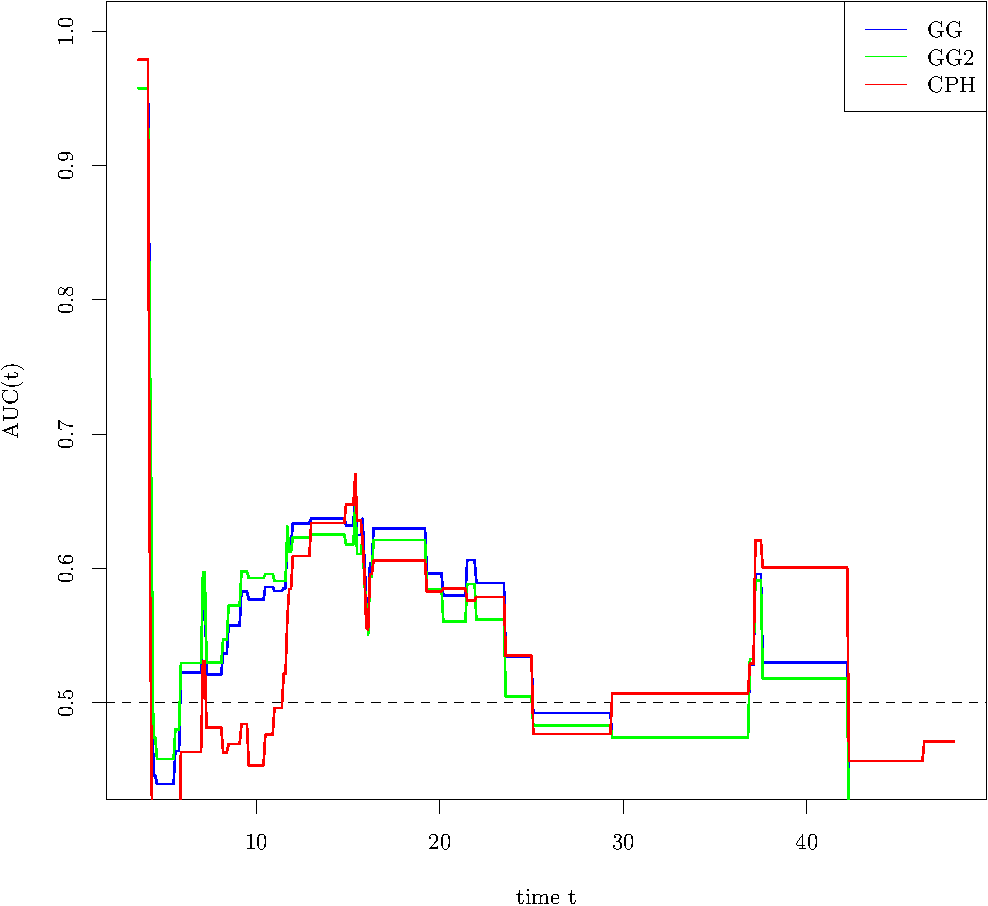
\includegraphics[width=\maxwidth]{figure/05-model-selection-auc-1} 

}


\begin{kframe}\begin{alltt}
\hlkwd{plot}\hlstd{(}\hlkwd{survfit}\hlstd{(}\hlkwd{Surv}\hlstd{(data.val}\hlopt{$}\hlstd{Time}\hlopt{/}\hlnum{365.25}\hlopt{*}\hlnum{12}\hlstd{, data.val}\hlopt{$}\hlstd{DSD)} \hlopt{~} \hlnum{1}\hlstd{))}
\hlkwd{abline}\hlstd{(}\hlkwc{v} \hlstd{=} \hlkwd{c}\hlstd{(}\hlnum{7}\hlstd{,} \hlnum{34}\hlstd{))}
\end{alltt}
\end{kframe}

{\centering \includegraphics[width=\maxwidth]{figure/05-model-selection-auc-2} 

}



\end{knitrout}


Decision curve analysis.
\begin{knitrout}
\definecolor{shadecolor}{rgb}{0.969, 0.969, 0.969}\color{fgcolor}\begin{kframe}
\begin{alltt}
\hlkwd{source}\hlstd{(}\hlstr{"stdca.R"}\hlstd{)}
\hlstd{temp.data} \hlkwb{=} \hlkwd{data.frame}\hlstd{(}\hlkwc{Time} \hlstd{= data.val}\hlopt{$}\hlstd{Time,} \hlkwc{DSD} \hlstd{= data.val}\hlopt{$}\hlstd{DSD}\hlopt{*}\hlnum{1}\hlstd{,}
    \hlkwc{gg.1} \hlstd{=} \hlnum{1}\hlopt{-}\hlstd{val.prob.gg[val.prob.times} \hlopt{==} \hlnum{365}\hlstd{,],} \hlkwc{gg.2} \hlstd{=} \hlnum{1}\hlopt{-}\hlstd{val.prob.gg[val.prob.times} \hlopt{==} \hlnum{365}\hlopt{*}\hlnum{2}\hlstd{,],} \hlkwc{gg.3} \hlstd{=} \hlnum{1}\hlopt{-}\hlstd{val.prob.gg[val.prob.times} \hlopt{==} \hlnum{365}\hlopt{*}\hlnum{3}\hlstd{,],}
    \hlkwc{gg2.1} \hlstd{=} \hlnum{1}\hlopt{-}\hlstd{val.prob.gg2[val.prob.times} \hlopt{==} \hlnum{365}\hlstd{,],} \hlkwc{gg2.2} \hlstd{=} \hlnum{1}\hlopt{-}\hlstd{val.prob.gg2[val.prob.times} \hlopt{==} \hlnum{365}\hlopt{*}\hlnum{2}\hlstd{,],} \hlkwc{gg2.3} \hlstd{=} \hlnum{1}\hlopt{-}\hlstd{val.prob.gg2[val.prob.times} \hlopt{==} \hlnum{365}\hlopt{*}\hlnum{3}\hlstd{,],}
    \hlkwc{cph.1} \hlstd{=} \hlnum{1}\hlopt{-}\hlstd{val.prob.cph[val.prob.times} \hlopt{==} \hlnum{365}\hlstd{,],} \hlkwc{cph.2} \hlstd{=} \hlnum{1}\hlopt{-}\hlstd{val.prob.cph[val.prob.times} \hlopt{==} \hlnum{365}\hlopt{*}\hlnum{2}\hlstd{,],} \hlkwc{cph.3} \hlstd{=} \hlnum{1}\hlopt{-}\hlstd{val.prob.cph[val.prob.times} \hlopt{==} \hlnum{365}\hlopt{*}\hlnum{3}\hlstd{,],}
    \hlkwc{rsf.1} \hlstd{=} \hlnum{1}\hlopt{-}\hlstd{val.prob.rsf[val.prob.times} \hlopt{==} \hlnum{365}\hlstd{,],} \hlkwc{rsf.2} \hlstd{=} \hlnum{1}\hlopt{-}\hlstd{val.prob.rsf[val.prob.times} \hlopt{==} \hlnum{365}\hlopt{*}\hlnum{2}\hlstd{,],} \hlkwc{rsf.3} \hlstd{=} \hlnum{1}\hlopt{-}\hlstd{val.prob.rsf[val.prob.times} \hlopt{==} \hlnum{365}\hlopt{*}\hlnum{3}\hlstd{,])}
\hlkwd{invisible}\hlstd{(}\hlkwd{stdca}\hlstd{(}\hlkwc{data} \hlstd{= temp.data,} \hlkwc{outcome} \hlstd{=} \hlstr{"DSD"}\hlstd{,} \hlkwc{ttoutcome} \hlstd{=} \hlstr{"Time"}\hlstd{,} \hlkwc{predictors} \hlstd{=} \hlkwd{c}\hlstd{(}\hlstr{"gg.1"}\hlstd{,} \hlstr{"gg2.1"}\hlstd{,} \hlstr{"cph.1"}\hlstd{,} \hlstr{"rsf.1"}\hlstd{),} \hlkwc{timepoint} \hlstd{=} \hlnum{365}\hlstd{,} \hlkwc{probability} \hlstd{=} \hlkwd{rep}\hlstd{(}\hlnum{TRUE}\hlstd{,} \hlnum{4}\hlstd{)))}
\end{alltt}
\begin{verbatim}
## [1] "gg.1: No observations with risk greater than 70% that have followup through the timepoint selected, and therefore net benefit not calculable in this range." 
## [2] "gg2.1: No observations with risk greater than 69% that have followup through the timepoint selected, and therefore net benefit not calculable in this range."
## [3] "cph.1: No observations with risk greater than 77% that have followup through the timepoint selected, and therefore net benefit not calculable in this range."
## [4] "rsf.1: No observations with risk greater than 64%, and therefore net benefit not calculable in this range."
\end{verbatim}
\end{kframe}

{\centering 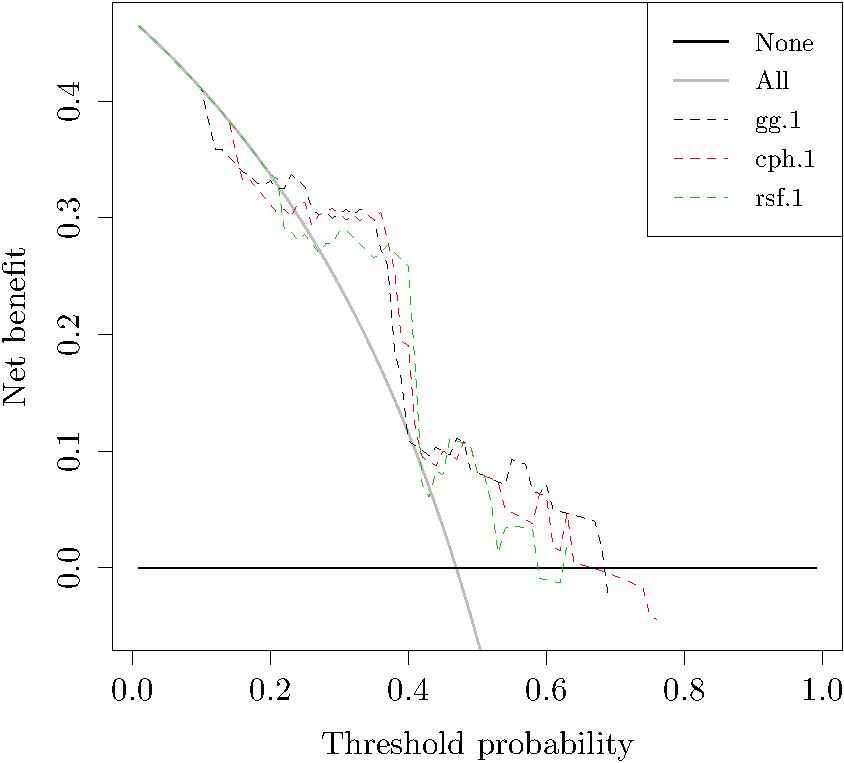
\includegraphics[width=\maxwidth]{figure/05-model-selection-dca-1} 

}


\begin{kframe}\begin{alltt}
\hlkwd{invisible}\hlstd{(}\hlkwd{stdca}\hlstd{(}\hlkwc{data} \hlstd{= temp.data,} \hlkwc{outcome} \hlstd{=} \hlstr{"DSD"}\hlstd{,} \hlkwc{ttoutcome} \hlstd{=} \hlstr{"Time"}\hlstd{,} \hlkwc{predictors} \hlstd{=} \hlkwd{c}\hlstd{(}\hlstr{"gg.2"}\hlstd{,} \hlstr{"gg2.2"}\hlstd{,} \hlstr{"cph.2"}\hlstd{,} \hlstr{"rsf.2"}\hlstd{),} \hlkwc{timepoint} \hlstd{=} \hlnum{365}\hlopt{*}\hlnum{2}\hlstd{,} \hlkwc{probability} \hlstd{=} \hlkwd{rep}\hlstd{(}\hlnum{TRUE}\hlstd{,} \hlnum{4}\hlstd{)))}
\end{alltt}
\begin{verbatim}
## [1] "gg.2: No observations with risk greater than 85% that have followup through the timepoint selected, and therefore net benefit not calculable in this range." 
## [2] "gg2.2: No observations with risk greater than 88% that have followup through the timepoint selected, and therefore net benefit not calculable in this range."
## [3] "cph.2: No observations with risk greater than 83% that have followup through the timepoint selected, and therefore net benefit not calculable in this range."
## [4] "rsf.2: No observations with risk greater than 72% that have followup through the timepoint selected, and therefore net benefit not calculable in this range."
\end{verbatim}
\end{kframe}

{\centering 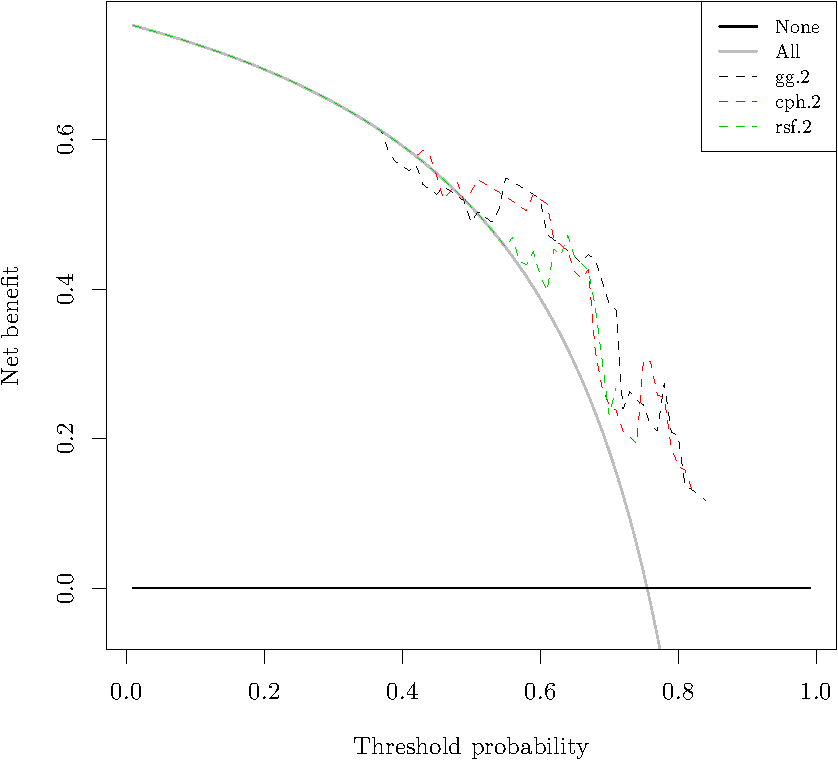
\includegraphics[width=\maxwidth]{figure/05-model-selection-dca-2} 

}


\begin{kframe}\begin{alltt}
\hlkwd{invisible}\hlstd{(}\hlkwd{stdca}\hlstd{(}\hlkwc{data} \hlstd{= temp.data,} \hlkwc{outcome} \hlstd{=} \hlstr{"DSD"}\hlstd{,} \hlkwc{ttoutcome} \hlstd{=} \hlstr{"Time"}\hlstd{,} \hlkwc{predictors} \hlstd{=} \hlkwd{c}\hlstd{(}\hlstr{"gg.3"}\hlstd{,} \hlstr{"gg2.3"}\hlstd{,} \hlstr{"cph.3"}\hlstd{,} \hlstr{"rsf.3"}\hlstd{),} \hlkwc{timepoint} \hlstd{=} \hlnum{365}\hlopt{*}\hlnum{3}\hlstd{,} \hlkwc{probability} \hlstd{=} \hlkwd{rep}\hlstd{(}\hlnum{TRUE}\hlstd{,} \hlnum{4}\hlstd{)))}
\end{alltt}
\begin{verbatim}
## [1] "gg.3: No observations with risk greater than 97% that have followup through the timepoint selected, and therefore net benefit not calculable in this range." 
## [2] "gg2.3: No observations with risk greater than 99% that have followup through the timepoint selected, and therefore net benefit not calculable in this range."
## [3] "cph.3: No observations with risk greater than 97% that have followup through the timepoint selected, and therefore net benefit not calculable in this range."
## [4] "rsf.3: No observations with risk greater than 90% that have followup through the timepoint selected, and therefore net benefit not calculable in this range."
\end{verbatim}
\end{kframe}

{\centering 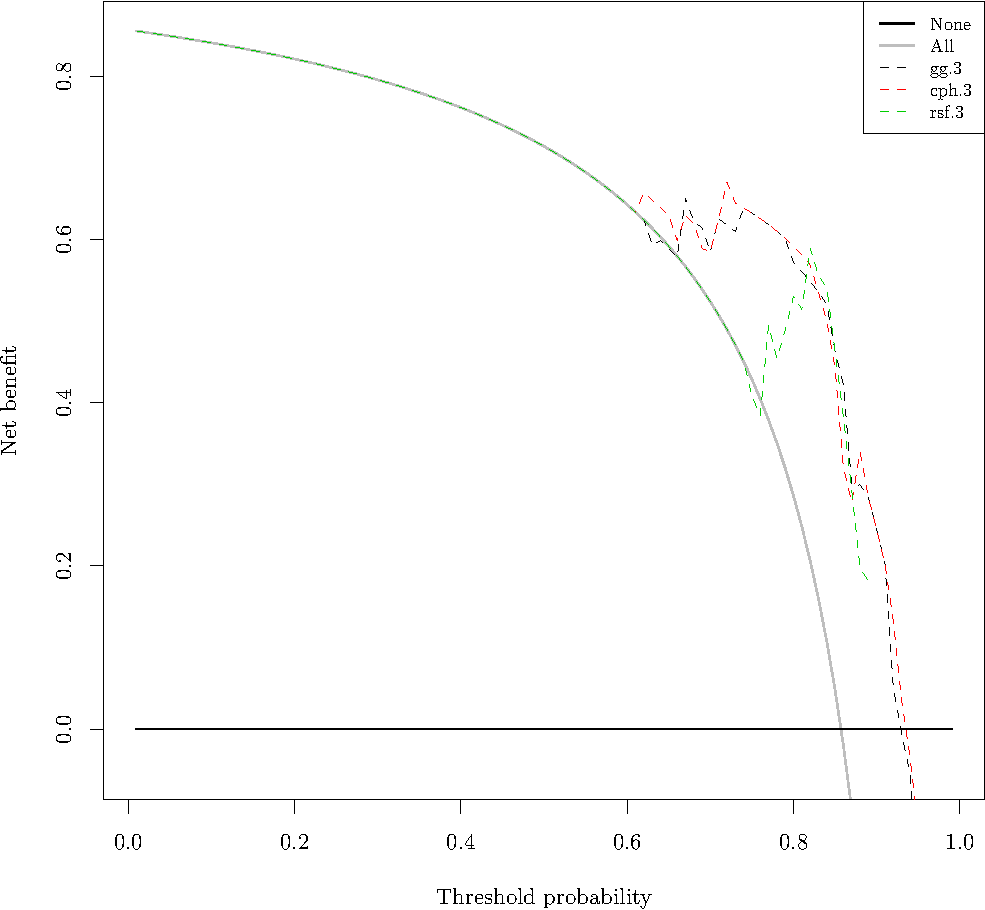
\includegraphics[width=\maxwidth]{figure/05-model-selection-dca-3} 

}



\end{knitrout}


Evaluate IBS point estimates.
BS paths over time on bootstrap samples of the holdout set.
\begin{knitrout}
\definecolor{shadecolor}{rgb}{0.969, 0.969, 0.969}\color{fgcolor}\begin{kframe}
\begin{alltt}
\hlkwd{set.seed}\hlstd{(}\hlnum{20150208}\hlstd{)}
\hlstd{ibs_eval_times} \hlkwb{=} \hlkwd{calcIBS}\hlstd{(}\hlkwd{Surv}\hlstd{(data.val}\hlopt{$}\hlstd{Time, data.val}\hlopt{$}\hlstd{DSD), ibs_preds_gg, ibs_times,} \hlkwd{max}\hlstd{(data.val}\hlopt{$}\hlstd{Time))}\hlopt{$}\hlstd{eval_times}
\hlstd{bsc_boots} \hlkwb{=} \hlkwd{laply}\hlstd{(}\hlnum{1}\hlopt{:}\hlnum{500}\hlstd{,} \hlkwa{function}\hlstd{(}\hlkwc{i}\hlstd{) \{}
        \hlkwa{if} \hlstd{(i} \hlopt \hlnum{50} \hlopt{==} \hlnum{0}\hlstd{)       \{} \hlkwd{message}\hlstd{(i) \}}
        \hlstd{boot_samp} \hlkwb{=} \hlkwd{sample.int}\hlstd{(}\hlkwd{nrow}\hlstd{(data.val),} \hlkwc{replace} \hlstd{=} \hlnum{TRUE}\hlstd{)}
        \hlstd{gg} \hlkwb{=} \hlkwd{calcIBS}\hlstd{(}\hlkwd{Surv}\hlstd{(data.val}\hlopt{$}\hlstd{Time, data.val}\hlopt{$}\hlstd{DSD)[boot_samp,], ibs_preds_gg[boot_samp,], ibs_times,} \hlkwd{max}\hlstd{(data.val}\hlopt{$}\hlstd{Time))}\hlopt{$}\hlstd{bsc}
        \hlstd{gg2} \hlkwb{=} \hlkwd{calcIBS}\hlstd{(}\hlkwd{Surv}\hlstd{(data.val}\hlopt{$}\hlstd{Time, data.val}\hlopt{$}\hlstd{DSD)[boot_samp,], ibs_preds_gg2[boot_samp,], ibs_times,} \hlkwd{max}\hlstd{(data.val}\hlopt{$}\hlstd{Time))}\hlopt{$}\hlstd{bsc}
        \hlstd{cph} \hlkwb{=} \hlkwd{calcIBS}\hlstd{(}\hlkwd{Surv}\hlstd{(data.val}\hlopt{$}\hlstd{Time, data.val}\hlopt{$}\hlstd{DSD)[boot_samp,], ibs_preds_cph[boot_samp,], ibs_times,} \hlkwd{max}\hlstd{(data.val}\hlopt{$}\hlstd{Time))}\hlopt{$}\hlstd{bsc}
        \hlstd{rsf} \hlkwb{=} \hlkwd{calcIBS}\hlstd{(}\hlkwd{Surv}\hlstd{(data.val}\hlopt{$}\hlstd{Time, data.val}\hlopt{$}\hlstd{DSD)[boot_samp,], ibs_preds_rsf[boot_samp,], ibs_times,} \hlkwd{max}\hlstd{(data.val}\hlopt{$}\hlstd{Time))}\hlopt{$}\hlstd{bsc}
        \hlstd{km0} \hlkwb{=} \hlkwd{calcIBS}\hlstd{(}\hlkwd{Surv}\hlstd{(data.val}\hlopt{$}\hlstd{Time, data.val}\hlopt{$}\hlstd{DSD)[boot_samp,], ibs_preds_km0[boot_samp,], ibs_times,} \hlkwd{max}\hlstd{(data.val}\hlopt{$}\hlstd{Time))}\hlopt{$}\hlstd{bsc}
        \hlkwd{rbind}\hlstd{(gg, gg2, cph, rsf, km0)}
\hlstd{\})}
\end{alltt}


{\ttfamily\noindent\itshape\color{messagecolor}{\#\# 50\\\#\# 100\\\#\# 150\\\#\# 200\\\#\# 250\\\#\# 300\\\#\# 350\\\#\# 400\\\#\# 450\\\#\# 500}}\end{kframe}
\end{knitrout}

\begin{knitrout}
\definecolor{shadecolor}{rgb}{0.969, 0.969, 0.969}\color{fgcolor}\begin{kframe}
\begin{alltt}
\hlstd{temp} \hlkwb{=} \hlkwd{sapply}\hlstd{(}\hlkwd{list}\hlstd{(}\hlkwc{gg} \hlstd{= ibs_preds_gg,} \hlkwc{gg2} \hlstd{= ibs_preds_gg2,} \hlkwc{cph} \hlstd{= ibs_preds_cph,} \hlkwc{rsf} \hlstd{= ibs_preds_rsf,} \hlkwc{km0} \hlstd{= ibs_preds_km0),} \hlkwa{function}\hlstd{(}\hlkwc{preds}\hlstd{)} \hlkwd{calcIBS}\hlstd{(}\hlkwd{Surv}\hlstd{(data.val}\hlopt{$}\hlstd{Time, data.val}\hlopt{$}\hlstd{DSD), preds, ibs_times,} \hlkwd{max}\hlstd{(data.val}\hlopt{$}\hlstd{Time))}\hlopt{$}\hlstd{bsc)}
\hlstd{temp} \hlkwb{=} \hlkwd{melt}\hlstd{(temp)}
\hlkwd{colnames}\hlstd{(temp)} \hlkwb{=} \hlkwd{c}\hlstd{(}\hlstr{"Time"}\hlstd{,} \hlstr{"Model"}\hlstd{,} \hlstr{"BS"}\hlstd{)}
\hlkwd{ggplot}\hlstd{(temp,} \hlkwd{aes}\hlstd{(}\hlkwc{x} \hlstd{= Time}\hlopt{/}\hlnum{365.25}\hlopt{*}\hlnum{12}\hlstd{,} \hlkwc{y} \hlstd{= BS,} \hlkwc{colour} \hlstd{= Model))} \hlopt{+} \hlkwd{geom_line}\hlstd{()} \hlopt{+} \hlkwd{ylab}\hlstd{(}\hlstr{"Brier Score"}\hlstd{)} \hlopt{+} \hlkwd{geom_hline}\hlstd{(}\hlkwc{yintercept} \hlstd{=} \hlnum{0.25}\hlstd{)} \hlopt{+} \hlkwd{geom_vline}\hlstd{(}\hlkwc{xintercept} \hlstd{=} \hlkwd{c}\hlstd{(}\hlnum{7}\hlstd{,} \hlnum{34}\hlstd{))}
\end{alltt}
\end{kframe}

{\centering 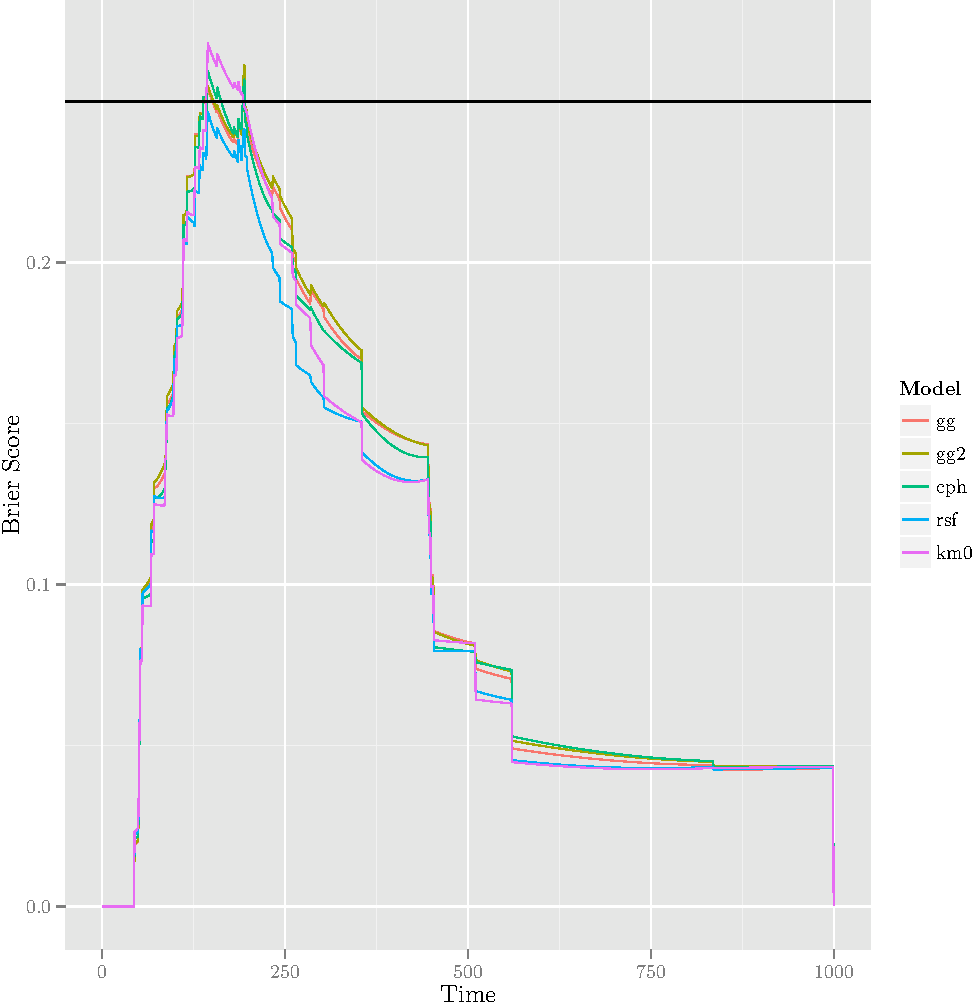
\includegraphics[width=\maxwidth]{figure/05-model-selection-bs-paths-1} 

}


\begin{kframe}\begin{alltt}
\hlstd{temp} \hlkwb{=} \hlkwd{melt}\hlstd{(}\hlkwd{aaply}\hlstd{(bsc_boots,} \hlnum{2}\hlopt{:}\hlnum{3}\hlstd{, quantile,} \hlkwc{probs} \hlstd{=} \hlkwd{c}\hlstd{(}\hlnum{0.05}\hlstd{,} \hlnum{0.5}\hlstd{,} \hlnum{0.95}\hlstd{)))}
\hlkwd{colnames}\hlstd{(temp)} \hlkwb{=} \hlkwd{c}\hlstd{(}\hlstr{"Model"}\hlstd{,} \hlstr{"Time"}\hlstd{,} \hlstr{"Quantile"}\hlstd{,} \hlstr{"Value"}\hlstd{)}
\hlstd{temp}\hlopt{$}\hlstd{Quantile} \hlkwb{=} \hlkwd{paste}\hlstd{(}\hlstr{"Q"}\hlstd{,} \hlkwd{gsub}\hlstd{(}\hlstr{"%"}\hlstd{,} \hlstr{""}\hlstd{, temp}\hlopt{$}\hlstd{Quantile),} \hlkwc{sep} \hlstd{=} \hlstr{""}\hlstd{)}
\hlstd{temp} \hlkwb{=} \hlkwd{dcast}\hlstd{(temp, Model} \hlopt{+} \hlstd{Time} \hlopt{~} \hlstd{Quantile,} \hlkwc{value.var} \hlstd{=} \hlstr{"Value"}\hlstd{)}
\hlkwd{ggplot}\hlstd{(temp,} \hlkwd{aes}\hlstd{(}\hlkwc{x} \hlstd{= Time}\hlopt{/}\hlnum{365.25}\hlopt{*}\hlnum{12}\hlstd{,} \hlkwc{y} \hlstd{= Q50,} \hlkwc{ymin} \hlstd{= Q5,} \hlkwc{ymax} \hlstd{= Q95,} \hlkwc{colour} \hlstd{= Model,} \hlkwc{fill} \hlstd{= Model))} \hlopt{+} \hlkwd{geom_line}\hlstd{()} \hlopt{+} \hlkwd{geom_ribbon}\hlstd{(}\hlkwc{alpha} \hlstd{=} \hlnum{0.2}\hlstd{,} \hlkwc{colour} \hlstd{=} \hlnum{NA}\hlstd{)} \hlopt{+} \hlkwd{ylab}\hlstd{(}\hlstr{"Brier Score, 90\textbackslash{}\textbackslash{}% BI"}\hlstd{)} \hlopt{+} \hlkwd{geom_hline}\hlstd{(}\hlkwc{yintercept} \hlstd{=} \hlnum{0.25}\hlstd{)} \hlopt{+} \hlkwd{geom_vline}\hlstd{(}\hlkwc{xintercept} \hlstd{=} \hlkwd{c}\hlstd{(}\hlnum{7}\hlstd{,} \hlnum{34}\hlstd{))}
\end{alltt}
\end{kframe}

{\centering 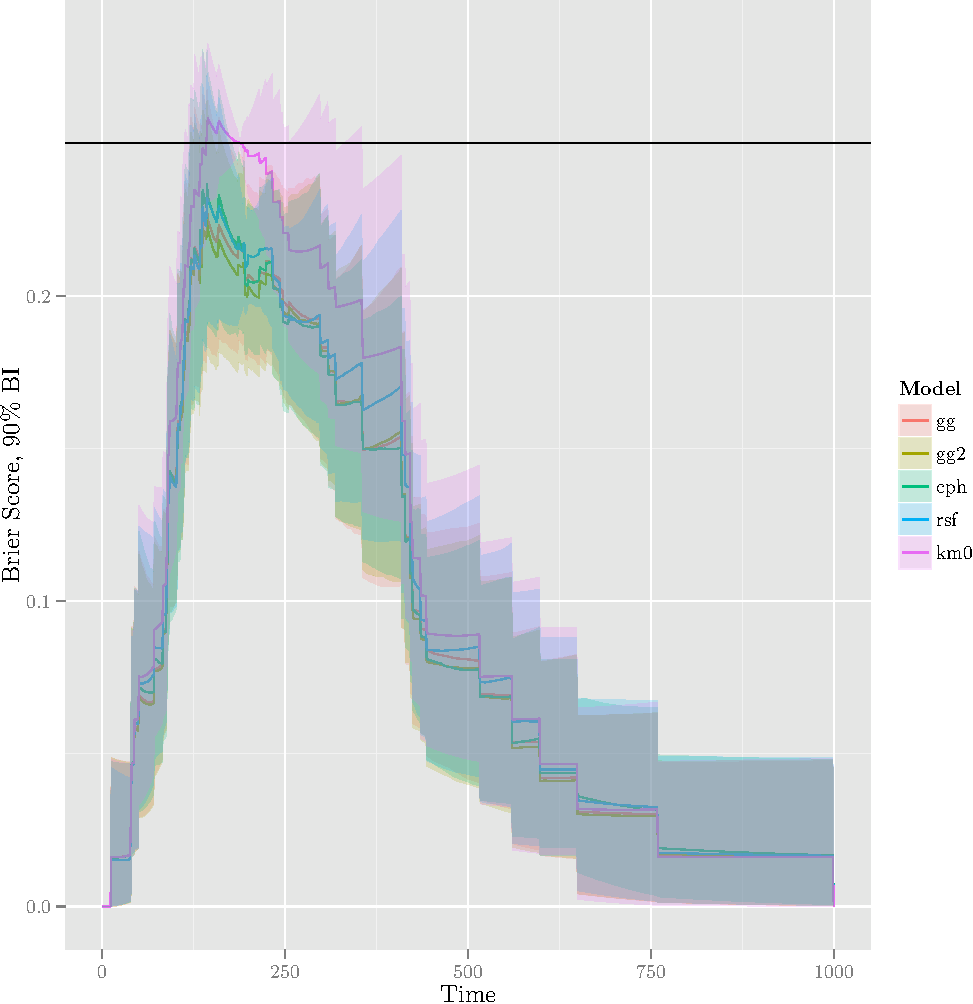
\includegraphics[width=\maxwidth]{figure/05-model-selection-bs-paths-2} 

}


\begin{kframe}\begin{alltt}
\hlstd{bsc_boots_diff} \hlkwb{=} \hlkwd{aaply}\hlstd{(bsc_boots,} \hlnum{2}\hlstd{,} \hlkwa{function}\hlstd{(}\hlkwc{x}\hlstd{) x} \hlopt{-} \hlstd{bsc_boots[,}\hlnum{5}\hlstd{,])[}\hlnum{1}\hlopt{:}\hlnum{4}\hlstd{,,]}
\hlstd{temp} \hlkwb{=} \hlkwd{melt}\hlstd{(}\hlkwd{aaply}\hlstd{(bsc_boots_diff,} \hlkwd{c}\hlstd{(}\hlnum{1}\hlstd{,}\hlnum{3}\hlstd{), quantile,} \hlkwc{probs} \hlstd{=} \hlkwd{c}\hlstd{(}\hlnum{0.05}\hlstd{,} \hlnum{0.5}\hlstd{,} \hlnum{0.95}\hlstd{)))}
\hlkwd{colnames}\hlstd{(temp)} \hlkwb{=} \hlkwd{c}\hlstd{(}\hlstr{"Model"}\hlstd{,} \hlstr{"Time"}\hlstd{,} \hlstr{"Quantile"}\hlstd{,} \hlstr{"Value"}\hlstd{)}
\hlstd{temp}\hlopt{$}\hlstd{Quantile} \hlkwb{=} \hlkwd{paste}\hlstd{(}\hlstr{"Q"}\hlstd{,} \hlkwd{gsub}\hlstd{(}\hlstr{"%"}\hlstd{,} \hlstr{""}\hlstd{, temp}\hlopt{$}\hlstd{Quantile),} \hlkwc{sep} \hlstd{=} \hlstr{""}\hlstd{)}
\hlstd{temp} \hlkwb{=} \hlkwd{dcast}\hlstd{(temp, Model} \hlopt{+} \hlstd{Time} \hlopt{~} \hlstd{Quantile,} \hlkwc{value.var} \hlstd{=} \hlstr{"Value"}\hlstd{)}
\hlkwd{ggplot}\hlstd{(temp,} \hlkwd{aes}\hlstd{(}\hlkwc{x} \hlstd{= Time}\hlopt{/}\hlnum{365.25}\hlopt{*}\hlnum{12}\hlstd{,} \hlkwc{y} \hlstd{= Q50,} \hlkwc{ymin} \hlstd{= Q5,} \hlkwc{ymax} \hlstd{= Q95,} \hlkwc{colour} \hlstd{= Model,} \hlkwc{fill} \hlstd{= Model))} \hlopt{+} \hlkwd{geom_line}\hlstd{()} \hlopt{+} \hlkwd{geom_ribbon}\hlstd{(}\hlkwc{alpha} \hlstd{=} \hlnum{0.2}\hlstd{,} \hlkwc{colour} \hlstd{=} \hlnum{NA}\hlstd{)} \hlopt{+} \hlkwd{ylab}\hlstd{(}\hlstr{"Brier Score: Improvement over KM0. BS median, 90\textbackslash{}\textbackslash{}% BI"}\hlstd{)} \hlopt{+} \hlkwd{geom_hline}\hlstd{(}\hlkwc{yintercept} \hlstd{=} \hlnum{0}\hlstd{)}
\end{alltt}
\end{kframe}

{\centering 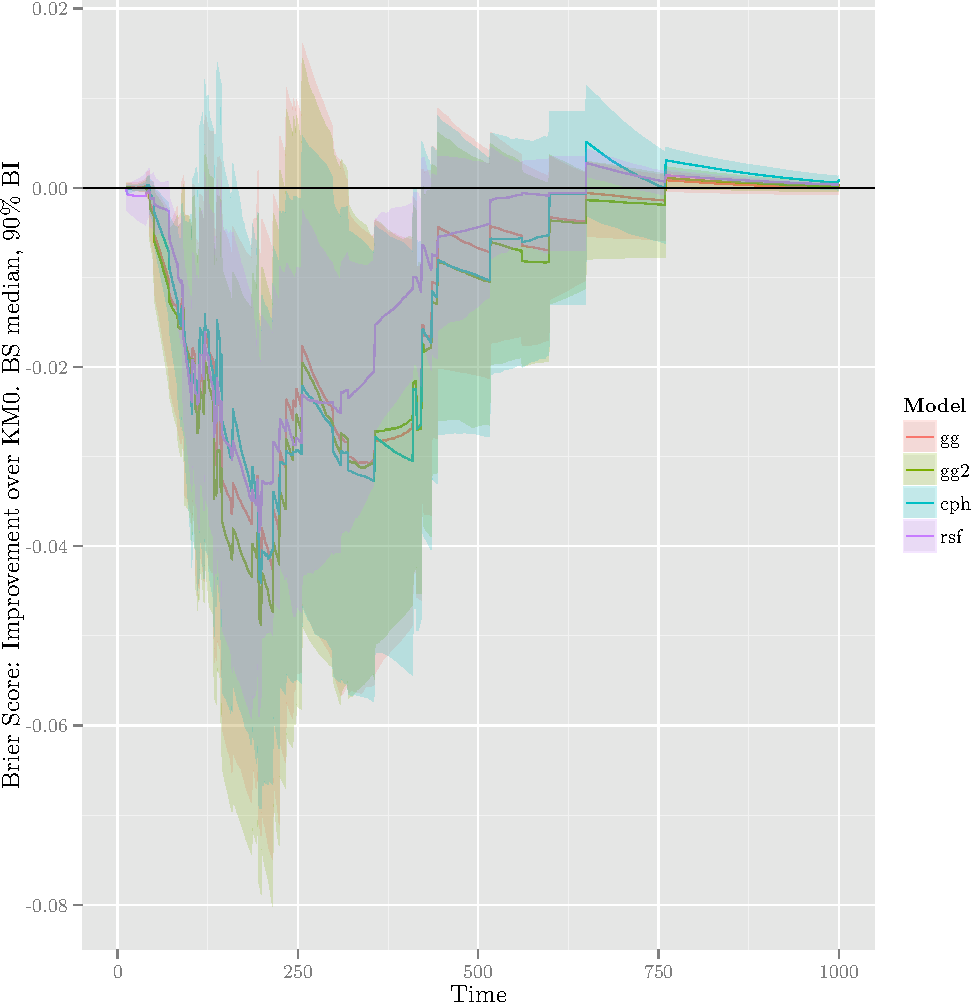
\includegraphics[width=\maxwidth]{figure/05-model-selection-bs-paths-3} 

}


\begin{kframe}\begin{alltt}
\hlkwd{ggplot}\hlstd{(temp,} \hlkwd{aes}\hlstd{(}\hlkwc{x} \hlstd{= Time}\hlopt{/}\hlnum{365.25}\hlopt{*}\hlnum{12}\hlstd{,} \hlkwc{y} \hlstd{= Q50,} \hlkwc{ymin} \hlstd{= Q5,} \hlkwc{ymax} \hlstd{= Q95,} \hlkwc{colour} \hlstd{= Model,} \hlkwc{fill} \hlstd{= Model))} \hlopt{+} \hlkwd{geom_line}\hlstd{()} \hlopt{+} \hlkwd{geom_ribbon}\hlstd{(}\hlkwc{alpha} \hlstd{=} \hlnum{0.2}\hlstd{,} \hlkwc{colour} \hlstd{=} \hlnum{NA}\hlstd{)} \hlopt{+} \hlkwd{xlim}\hlstd{(}\hlnum{0}\hlstd{,} \hlnum{34}\hlstd{)} \hlopt{+} \hlkwd{ylab}\hlstd{(}\hlstr{"Brier Score: Improvement over KM0. BS median, 90\textbackslash{}\textbackslash{}% BI"}\hlstd{)} \hlopt{+} \hlkwd{geom_hline}\hlstd{(}\hlkwc{yintercept} \hlstd{=} \hlnum{0}\hlstd{)}
\end{alltt}
\end{kframe}

{\centering 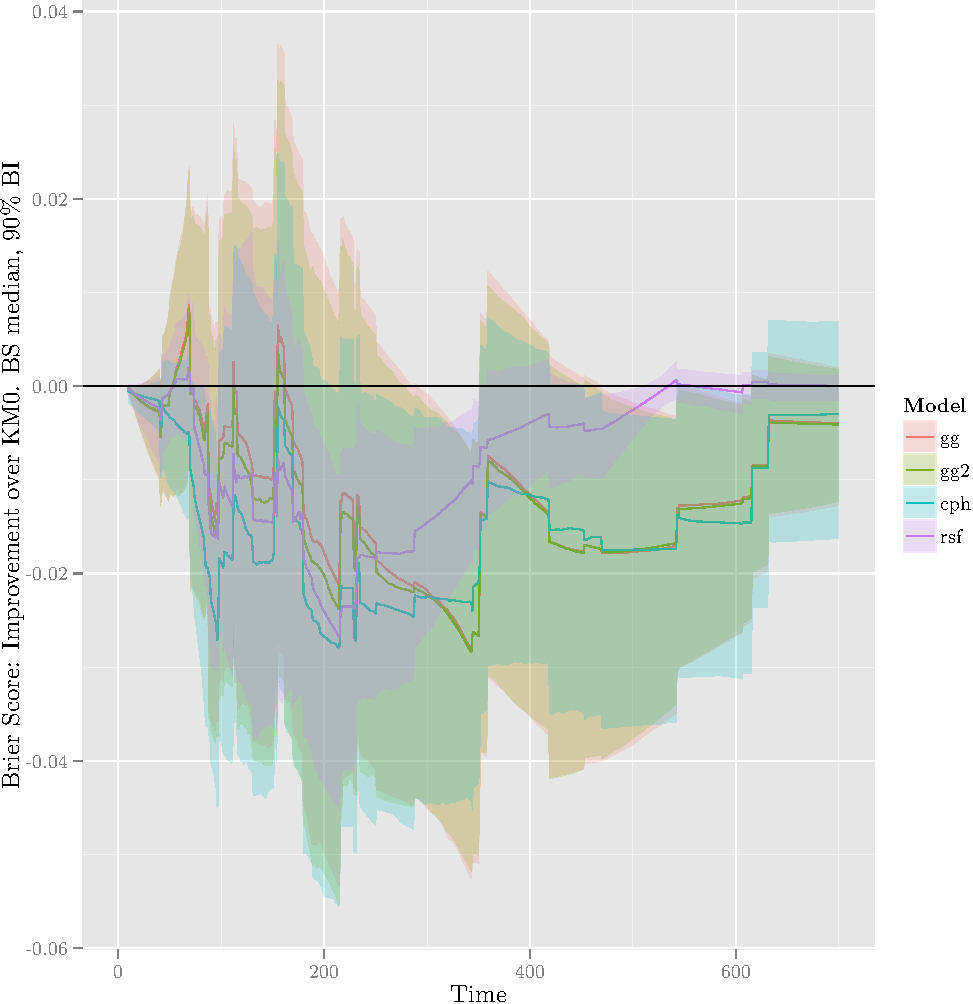
\includegraphics[width=\maxwidth]{figure/05-model-selection-bs-paths-4} 

}


\begin{kframe}\begin{alltt}
\hlkwd{ggplot}\hlstd{(temp,} \hlkwd{aes}\hlstd{(}\hlkwc{x} \hlstd{= Time}\hlopt{/}\hlnum{365.25}\hlopt{*}\hlnum{12}\hlstd{,} \hlkwc{y} \hlstd{= Q50,} \hlkwc{colour} \hlstd{= Model))} \hlopt{+} \hlkwd{geom_line}\hlstd{()} \hlopt{+} \hlkwd{ylab}\hlstd{(}\hlstr{"Brier Score: Improvement over KM0, BS median"}\hlstd{)} \hlopt{+} \hlkwd{geom_hline}\hlstd{(}\hlkwc{yintercept} \hlstd{=} \hlnum{0}\hlstd{)} \hlopt{+} \hlkwd{geom_vline}\hlstd{(}\hlkwc{xintercept} \hlstd{=} \hlkwd{c}\hlstd{(}\hlnum{7}\hlstd{,} \hlnum{34}\hlstd{))}
\end{alltt}
\end{kframe}

{\centering 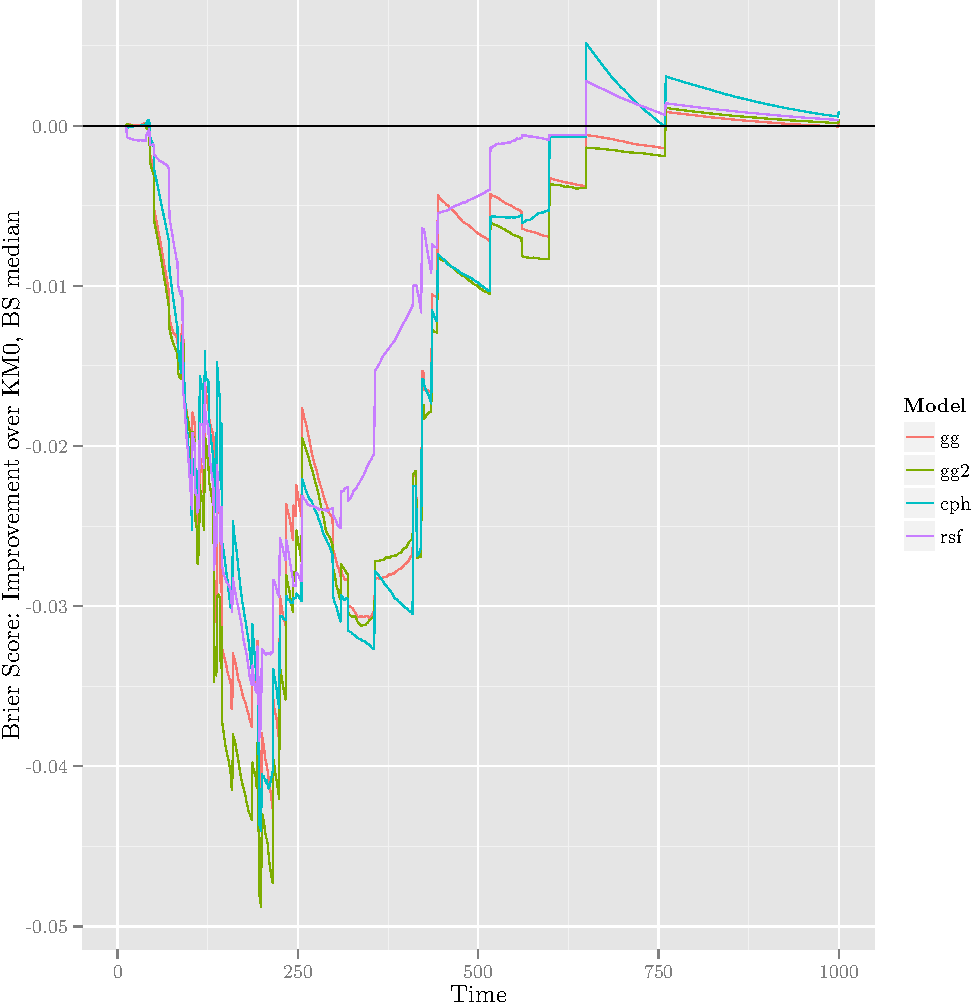
\includegraphics[width=\maxwidth]{figure/05-model-selection-bs-paths-5} 

}


\begin{kframe}\begin{alltt}
\hlkwd{ggplot}\hlstd{(temp,} \hlkwd{aes}\hlstd{(}\hlkwc{x} \hlstd{= Time}\hlopt{/}\hlnum{365.25}\hlopt{*}\hlnum{12}\hlstd{,} \hlkwc{y} \hlstd{= Q50,} \hlkwc{colour} \hlstd{= Model))} \hlopt{+} \hlkwd{geom_line}\hlstd{()} \hlopt{+} \hlkwd{ylab}\hlstd{(}\hlstr{"Brier Score: Improvement over KM0, BS median"}\hlstd{)} \hlopt{+} \hlkwd{xlim}\hlstd{(}\hlnum{0}\hlstd{,} \hlnum{34}\hlstd{)} \hlopt{+} \hlkwd{geom_hline}\hlstd{(}\hlkwc{yintercept} \hlstd{=} \hlnum{0}\hlstd{)} \hlopt{+} \hlkwd{geom_vline}\hlstd{(}\hlkwc{xintercept} \hlstd{=} \hlkwd{c}\hlstd{(}\hlnum{7}\hlstd{,} \hlnum{34}\hlstd{))}
\end{alltt}
\end{kframe}

{\centering 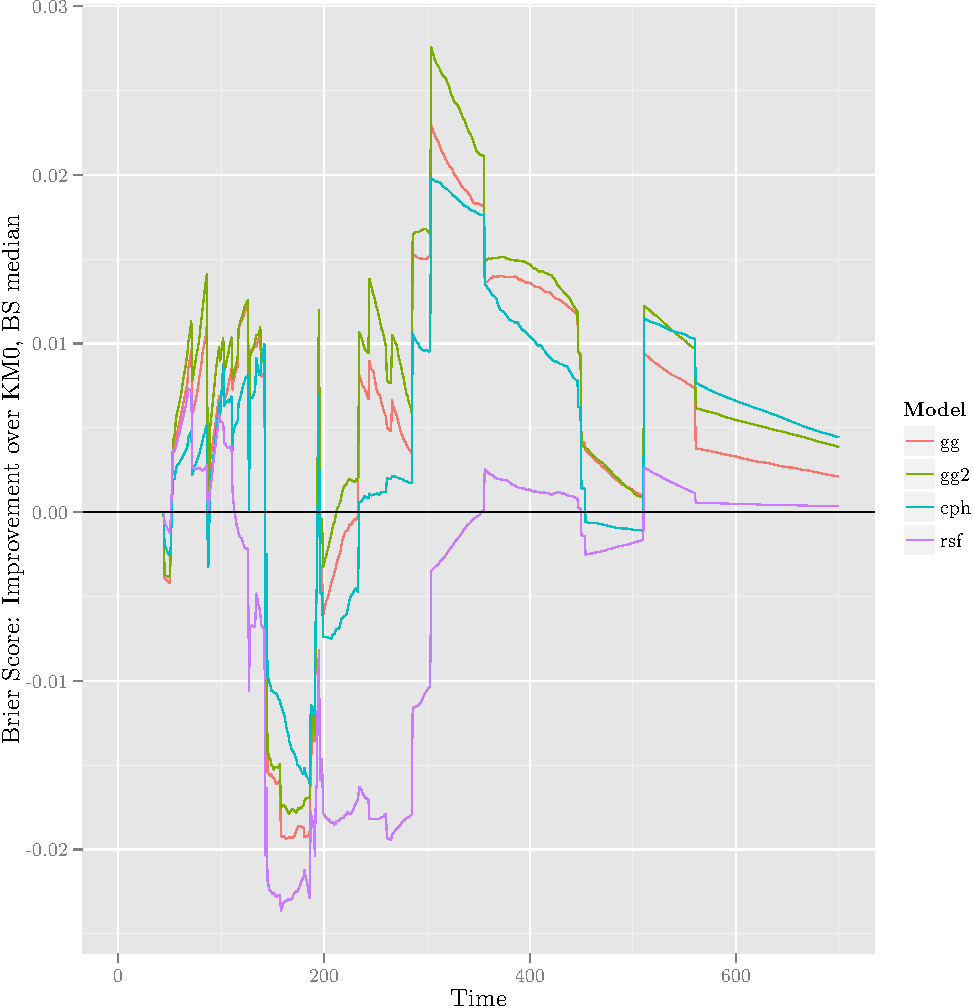
\includegraphics[width=\maxwidth]{figure/05-model-selection-bs-paths-6} 

}



\end{knitrout}

IBS comparisons.
\begin{knitrout}
\definecolor{shadecolor}{rgb}{0.969, 0.969, 0.969}\color{fgcolor}\begin{kframe}
\begin{alltt}
\hlkwd{set.seed}\hlstd{(}\hlnum{20150208}\hlstd{)}
\hlstd{ibsc_boots} \hlkwb{=} \hlkwd{t}\hlstd{(}\hlkwd{sapply}\hlstd{(}\hlnum{1}\hlopt{:}\hlnum{5e2}\hlstd{,} \hlkwa{function}\hlstd{(}\hlkwc{i}\hlstd{) \{}
        \hlkwa{if} \hlstd{(i} \hlopt \hlnum{5e1} \hlopt{==} \hlnum{0}\hlstd{)      \{} \hlkwd{message}\hlstd{(i) \}}
        \hlstd{boot_samp} \hlkwb{=} \hlkwd{sample.int}\hlstd{(}\hlkwd{nrow}\hlstd{(data.val),} \hlkwc{replace} \hlstd{=} \hlnum{TRUE}\hlstd{)}
        \hlstd{gg} \hlkwb{=} \hlkwd{calcIBS}\hlstd{(}\hlkwd{Surv}\hlstd{(data.val}\hlopt{$}\hlstd{Time, data.val}\hlopt{$}\hlstd{DSD)[boot_samp,], ibs_preds_gg[boot_samp,], ibs_times,} \hlnum{34}\hlopt{*}\hlnum{365.25}\hlopt{/}\hlnum{12}\hlstd{,} \hlnum{7}\hlopt{*}\hlnum{365.25}\hlopt{/}\hlnum{12}\hlstd{)}\hlopt{$}\hlstd{ibs}
        \hlstd{gg2} \hlkwb{=} \hlkwd{calcIBS}\hlstd{(}\hlkwd{Surv}\hlstd{(data.val}\hlopt{$}\hlstd{Time, data.val}\hlopt{$}\hlstd{DSD)[boot_samp,], ibs_preds_gg2[boot_samp,], ibs_times,} \hlnum{34}\hlopt{*}\hlnum{365.25}\hlopt{/}\hlnum{12}\hlstd{,} \hlnum{7}\hlopt{*}\hlnum{365.25}\hlopt{/}\hlnum{12}\hlstd{)}\hlopt{$}\hlstd{ibs}
        \hlstd{cph} \hlkwb{=} \hlkwd{calcIBS}\hlstd{(}\hlkwd{Surv}\hlstd{(data.val}\hlopt{$}\hlstd{Time, data.val}\hlopt{$}\hlstd{DSD)[boot_samp,], ibs_preds_cph[boot_samp,], ibs_times,} \hlnum{34}\hlopt{*}\hlnum{365.25}\hlopt{/}\hlnum{12}\hlstd{,} \hlnum{7}\hlopt{*}\hlnum{365.25}\hlopt{/}\hlnum{12}\hlstd{)}\hlopt{$}\hlstd{ibs}
        \hlstd{rsf} \hlkwb{=} \hlkwd{calcIBS}\hlstd{(}\hlkwd{Surv}\hlstd{(data.val}\hlopt{$}\hlstd{Time, data.val}\hlopt{$}\hlstd{DSD)[boot_samp,], ibs_preds_rsf[boot_samp,], ibs_times,} \hlnum{34}\hlopt{*}\hlnum{365.25}\hlopt{/}\hlnum{12}\hlstd{,} \hlnum{7}\hlopt{*}\hlnum{365.25}\hlopt{/}\hlnum{12}\hlstd{)}\hlopt{$}\hlstd{ibs}
        \hlstd{km0} \hlkwb{=} \hlkwd{calcIBS}\hlstd{(}\hlkwd{Surv}\hlstd{(data.val}\hlopt{$}\hlstd{Time, data.val}\hlopt{$}\hlstd{DSD)[boot_samp,], ibs_preds_km0[boot_samp,], ibs_times,} \hlnum{34}\hlopt{*}\hlnum{365.25}\hlopt{/}\hlnum{12}\hlstd{,} \hlnum{7}\hlopt{*}\hlnum{365.25}\hlopt{/}\hlnum{12}\hlstd{)}\hlopt{$}\hlstd{ibs}
        \hlkwd{c}\hlstd{(gg, gg2, cph, rsf, km0)}
\hlstd{\}))}
\end{alltt}


{\ttfamily\noindent\itshape\color{messagecolor}{\#\# 50\\\#\# 100\\\#\# 150\\\#\# 200\\\#\# 250\\\#\# 300\\\#\# 350\\\#\# 400\\\#\# 450\\\#\# 500}}\begin{alltt}
\hlkwd{colnames}\hlstd{(ibsc_boots)} \hlkwb{=} \hlkwd{c}\hlstd{(}\hlstr{"gg"}\hlstd{,} \hlstr{"gg2"}\hlstd{,} \hlstr{"cph"}\hlstd{,} \hlstr{"rsf"}\hlstd{,} \hlstr{"km0"}\hlstd{)}
\end{alltt}
\end{kframe}
\end{knitrout}

\begin{knitrout}
\definecolor{shadecolor}{rgb}{0.969, 0.969, 0.969}\color{fgcolor}\begin{kframe}
\begin{alltt}
\hlkwd{calcIBS}\hlstd{(}\hlkwd{Surv}\hlstd{(data.val}\hlopt{$}\hlstd{Time, data.val}\hlopt{$}\hlstd{DSD), ibs_preds_gg, ibs_times,} \hlnum{34}\hlopt{*}\hlnum{365.25}\hlopt{/}\hlnum{12}\hlstd{,} \hlnum{7}\hlopt{*}\hlnum{365.25}\hlopt{/}\hlnum{12}\hlstd{)}\hlopt{$}\hlstd{ibs}
\end{alltt}
\begin{verbatim}
## [1] 108
\end{verbatim}
\begin{alltt}
\hlkwd{calcIBS}\hlstd{(}\hlkwd{Surv}\hlstd{(data.val}\hlopt{$}\hlstd{Time, data.val}\hlopt{$}\hlstd{DSD), ibs_preds_gg2, ibs_times,} \hlnum{34}\hlopt{*}\hlnum{365.25}\hlopt{/}\hlnum{12}\hlstd{,} \hlnum{7}\hlopt{*}\hlnum{365.25}\hlopt{/}\hlnum{12}\hlstd{)}\hlopt{$}\hlstd{ibs}
\end{alltt}
\begin{verbatim}
## [1] 110.1
\end{verbatim}
\begin{alltt}
\hlkwd{calcIBS}\hlstd{(}\hlkwd{Surv}\hlstd{(data.val}\hlopt{$}\hlstd{Time, data.val}\hlopt{$}\hlstd{DSD), ibs_preds_cph, ibs_times,} \hlnum{34}\hlopt{*}\hlnum{365.25}\hlopt{/}\hlnum{12}\hlstd{,} \hlnum{7}\hlopt{*}\hlnum{365.25}\hlopt{/}\hlnum{12}\hlstd{)}\hlopt{$}\hlstd{ibs}
\end{alltt}
\begin{verbatim}
## [1] 108.8
\end{verbatim}
\begin{alltt}
\hlkwd{calcIBS}\hlstd{(}\hlkwd{Surv}\hlstd{(data.val}\hlopt{$}\hlstd{Time, data.val}\hlopt{$}\hlstd{DSD), ibs_preds_rsf, ibs_times,} \hlnum{34}\hlopt{*}\hlnum{365.25}\hlopt{/}\hlnum{12}\hlstd{,} \hlnum{7}\hlopt{*}\hlnum{365.25}\hlopt{/}\hlnum{12}\hlstd{)}\hlopt{$}\hlstd{ibs}
\end{alltt}
\begin{verbatim}
## [1] 114.5
\end{verbatim}
\begin{alltt}
\hlkwd{calcIBS}\hlstd{(}\hlkwd{Surv}\hlstd{(data.val}\hlopt{$}\hlstd{Time, data.val}\hlopt{$}\hlstd{DSD), ibs_preds_km0, ibs_times,} \hlnum{34}\hlopt{*}\hlnum{365.25}\hlopt{/}\hlnum{12}\hlstd{,} \hlnum{7}\hlopt{*}\hlnum{365.25}\hlopt{/}\hlnum{12}\hlstd{)}\hlopt{$}\hlstd{ibs}
\end{alltt}
\begin{verbatim}
## [1] 129
\end{verbatim}
\begin{alltt}
\hlkwd{boxplot}\hlstd{(ibsc_boots,} \hlkwc{main} \hlstd{=} \hlstr{"IBS BS Distribution"}\hlstd{,} \hlkwc{ylab} \hlstd{=} \hlstr{"IBS"}\hlstd{)}
\end{alltt}
\end{kframe}

{\centering 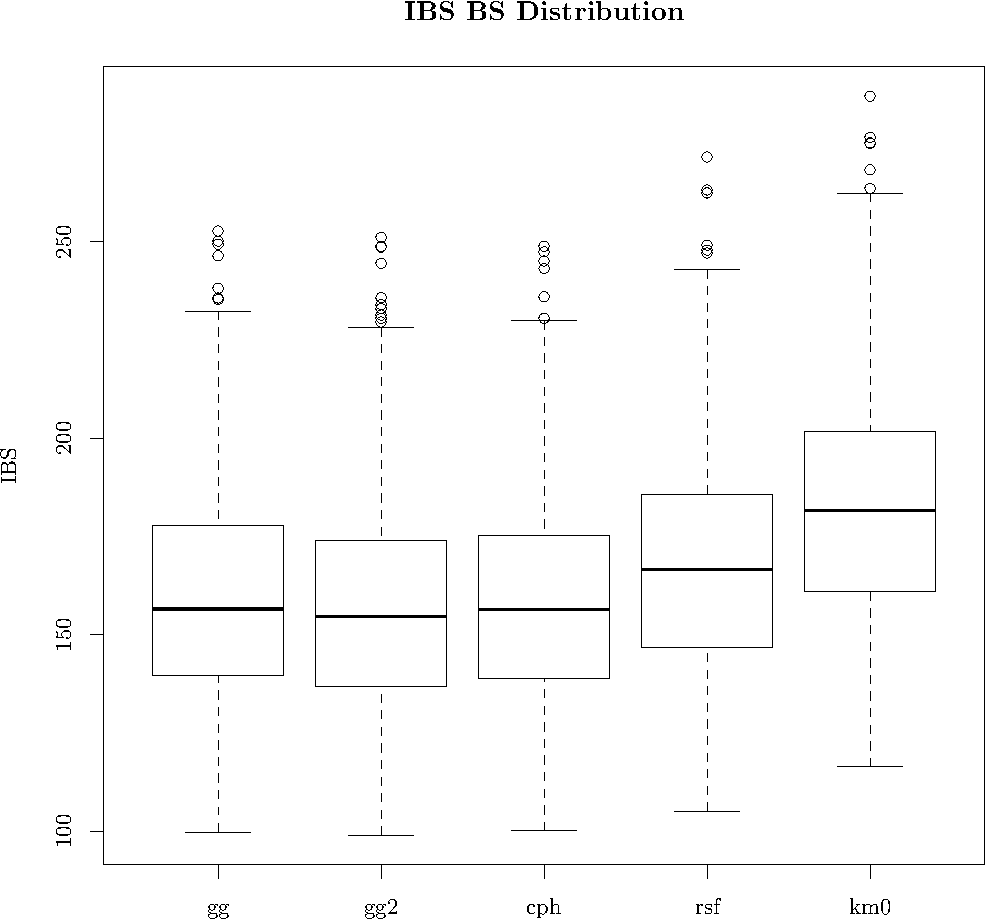
\includegraphics[width=\maxwidth]{figure/05-model-selection-ibs-1} 

}


\begin{kframe}\begin{alltt}
\hlkwd{plot}\hlstd{(}\hlkwd{density}\hlstd{(ibsc_boots[,}\hlnum{1}\hlstd{]),} \hlkwc{col} \hlstd{= pal[}\hlstr{"GG"}\hlstd{],} \hlkwc{lwd} \hlstd{=} \hlnum{2}\hlstd{,} \hlkwc{main} \hlstd{=} \hlstr{"IBS BS Distribution"}\hlstd{,} \hlkwc{xlab} \hlstd{=} \hlstr{"IBS"}\hlstd{)}
\hlkwd{lines}\hlstd{(}\hlkwd{density}\hlstd{(ibsc_boots[,}\hlnum{2}\hlstd{]),} \hlkwc{col} \hlstd{= pal[}\hlstr{"GG2"}\hlstd{],} \hlkwc{lwd} \hlstd{=} \hlnum{2}\hlstd{)}
\hlkwd{lines}\hlstd{(}\hlkwd{density}\hlstd{(ibsc_boots[,}\hlnum{3}\hlstd{]),} \hlkwc{col} \hlstd{= pal[}\hlstr{"CPH"}\hlstd{],} \hlkwc{lwd} \hlstd{=} \hlnum{2}\hlstd{)}
\hlkwd{lines}\hlstd{(}\hlkwd{density}\hlstd{(ibsc_boots[,}\hlnum{4}\hlstd{]),} \hlkwc{col} \hlstd{= pal[}\hlstr{"RSF"}\hlstd{],} \hlkwc{lwd} \hlstd{=} \hlnum{2}\hlstd{)}
\hlkwd{lines}\hlstd{(}\hlkwd{density}\hlstd{(ibsc_boots[,}\hlnum{4}\hlstd{]),} \hlkwc{col} \hlstd{= pal[}\hlstr{"KM0"}\hlstd{],} \hlkwc{lwd} \hlstd{=} \hlnum{2}\hlstd{)}
\hlkwd{abline}\hlstd{(}\hlkwc{v} \hlstd{=} \hlkwd{calcIBS}\hlstd{(}\hlkwd{Surv}\hlstd{(data.val}\hlopt{$}\hlstd{Time, data.val}\hlopt{$}\hlstd{DSD), ibs_preds_gg, ibs_times,} \hlnum{34}\hlopt{*}\hlnum{365.25}\hlopt{/}\hlnum{12}\hlstd{,} \hlnum{7}\hlopt{*}\hlnum{365.25}\hlopt{/}\hlnum{12}\hlstd{)}\hlopt{$}\hlstd{ibs,} \hlkwc{col} \hlstd{= pal[}\hlstr{"GG"}\hlstd{],} \hlkwc{lwd} \hlstd{=} \hlnum{1}\hlstd{)}
\hlkwd{abline}\hlstd{(}\hlkwc{v} \hlstd{=} \hlkwd{calcIBS}\hlstd{(}\hlkwd{Surv}\hlstd{(data.val}\hlopt{$}\hlstd{Time, data.val}\hlopt{$}\hlstd{DSD), ibs_preds_gg2, ibs_times,} \hlnum{34}\hlopt{*}\hlnum{365.25}\hlopt{/}\hlnum{12}\hlstd{,} \hlnum{7}\hlopt{*}\hlnum{365.25}\hlopt{/}\hlnum{12}\hlstd{)}\hlopt{$}\hlstd{ibs,} \hlkwc{col} \hlstd{= pal[}\hlstr{"GG2"}\hlstd{],} \hlkwc{lwd} \hlstd{=} \hlnum{1}\hlstd{)}
\hlkwd{abline}\hlstd{(}\hlkwc{v} \hlstd{=} \hlkwd{calcIBS}\hlstd{(}\hlkwd{Surv}\hlstd{(data.val}\hlopt{$}\hlstd{Time, data.val}\hlopt{$}\hlstd{DSD), ibs_preds_cph, ibs_times,} \hlnum{34}\hlopt{*}\hlnum{365.25}\hlopt{/}\hlnum{12}\hlstd{,} \hlnum{7}\hlopt{*}\hlnum{365.25}\hlopt{/}\hlnum{12}\hlstd{)}\hlopt{$}\hlstd{ibs,} \hlkwc{col} \hlstd{= pal[}\hlstr{"CPH"}\hlstd{],} \hlkwc{lwd} \hlstd{=} \hlnum{1}\hlstd{)}
\hlkwd{abline}\hlstd{(}\hlkwc{v} \hlstd{=} \hlkwd{calcIBS}\hlstd{(}\hlkwd{Surv}\hlstd{(data.val}\hlopt{$}\hlstd{Time, data.val}\hlopt{$}\hlstd{DSD), ibs_preds_rsf, ibs_times,} \hlnum{34}\hlopt{*}\hlnum{365.25}\hlopt{/}\hlnum{12}\hlstd{,} \hlnum{7}\hlopt{*}\hlnum{365.25}\hlopt{/}\hlnum{12}\hlstd{)}\hlopt{$}\hlstd{ibs,} \hlkwc{col} \hlstd{= pal[}\hlstr{"RSF"}\hlstd{],} \hlkwc{lwd} \hlstd{=} \hlnum{1}\hlstd{)}
\hlkwd{abline}\hlstd{(}\hlkwc{v} \hlstd{=} \hlkwd{calcIBS}\hlstd{(}\hlkwd{Surv}\hlstd{(data.val}\hlopt{$}\hlstd{Time, data.val}\hlopt{$}\hlstd{DSD), ibs_preds_km0, ibs_times,} \hlnum{34}\hlopt{*}\hlnum{365.25}\hlopt{/}\hlnum{12}\hlstd{,} \hlnum{7}\hlopt{*}\hlnum{365.25}\hlopt{/}\hlnum{12}\hlstd{)}\hlopt{$}\hlstd{ibs,} \hlkwc{col} \hlstd{= pal[}\hlstr{"KM0"}\hlstd{],} \hlkwc{lwd} \hlstd{=} \hlnum{1}\hlstd{)}
\hlkwd{legend}\hlstd{(}\hlstr{"topright"}\hlstd{,} \hlkwc{legend} \hlstd{=} \hlkwd{c}\hlstd{(}\hlstr{"GG"}\hlstd{,} \hlstr{"GG2"}\hlstd{,} \hlstr{"CPH"}\hlstd{,} \hlstr{"RSF"}\hlstd{,} \hlstr{"KM0"}\hlstd{),} \hlkwc{col} \hlstd{= pal[}\hlkwd{c}\hlstd{(}\hlstr{"GG"}\hlstd{,} \hlstr{"GG2"}\hlstd{,} \hlstr{"CPH"}\hlstd{,} \hlstr{"RSF"}\hlstd{,} \hlstr{"KM0"}\hlstd{)],} \hlkwc{lty} \hlstd{=} \hlstr{"solid"}\hlstd{,} \hlkwc{inset} \hlstd{=} \hlnum{0.05}\hlstd{)}
\end{alltt}
\end{kframe}

{\centering 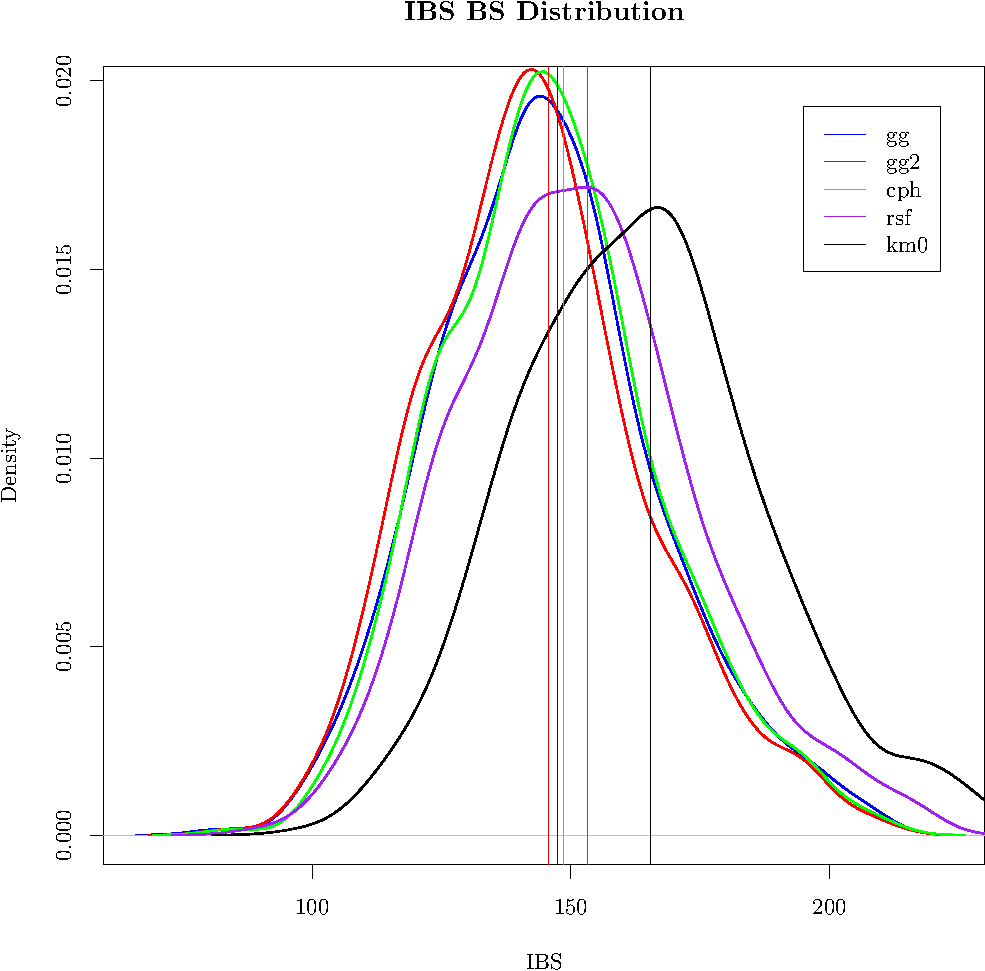
\includegraphics[width=\maxwidth]{figure/05-model-selection-ibs-2} 

}


\begin{kframe}\begin{alltt}
\hlkwd{plot}\hlstd{(}\hlkwd{density}\hlstd{(ibsc_boots[,}\hlnum{5}\hlstd{]} \hlopt{-} \hlstd{ibsc_boots[,}\hlnum{1}\hlstd{]),} \hlkwc{col} \hlstd{= pal[}\hlstr{"GG"}\hlstd{],} \hlkwc{lwd} \hlstd{=} \hlnum{2}\hlstd{,} \hlkwc{main} \hlstd{=} \hlstr{"IBS\textbackslash{}\textbackslash{}_KM0 - IBS\textbackslash{}\textbackslash{}_x BS Distribution"}\hlstd{,} \hlkwc{xlab} \hlstd{=} \hlstr{"IBS"}\hlstd{,} \hlkwc{ylim} \hlstd{=} \hlkwd{c}\hlstd{(}\hlnum{0}\hlstd{,} \hlnum{0.1}\hlstd{))}
\hlkwd{lines}\hlstd{(}\hlkwd{density}\hlstd{(ibsc_boots[,}\hlnum{5}\hlstd{]} \hlopt{-} \hlstd{ibsc_boots[,}\hlnum{2}\hlstd{]),} \hlkwc{col} \hlstd{= pal[}\hlstr{"GG2"}\hlstd{],} \hlkwc{lwd} \hlstd{=} \hlnum{2}\hlstd{)}
\hlkwd{lines}\hlstd{(}\hlkwd{density}\hlstd{(ibsc_boots[,}\hlnum{5}\hlstd{]} \hlopt{-} \hlstd{ibsc_boots[,}\hlnum{3}\hlstd{]),} \hlkwc{col} \hlstd{= pal[}\hlstr{"CPH"}\hlstd{],} \hlkwc{lwd} \hlstd{=} \hlnum{2}\hlstd{)}
\hlkwd{lines}\hlstd{(}\hlkwd{density}\hlstd{(ibsc_boots[,}\hlnum{5}\hlstd{]} \hlopt{-} \hlstd{ibsc_boots[,}\hlnum{4}\hlstd{]),} \hlkwc{col} \hlstd{= pal[}\hlstr{"RSF"}\hlstd{],} \hlkwc{lwd} \hlstd{=} \hlnum{2}\hlstd{)}
\hlkwd{abline}\hlstd{(}\hlkwc{v} \hlstd{= (}\hlkwd{calcIBS}\hlstd{(}\hlkwd{Surv}\hlstd{(data.val}\hlopt{$}\hlstd{Time, data.val}\hlopt{$}\hlstd{DSD), ibs_preds_km0, ibs_times,} \hlkwd{max}\hlstd{(data.val}\hlopt{$}\hlstd{Time))}\hlopt{$}\hlstd{ibs} \hlopt{-} \hlkwd{calcIBS}\hlstd{(}\hlkwd{Surv}\hlstd{(data.val}\hlopt{$}\hlstd{Time, data.val}\hlopt{$}\hlstd{DSD), ibs_preds_gg, ibs_times,} \hlkwd{max}\hlstd{(data.val}\hlopt{$}\hlstd{Time))}\hlopt{$}\hlstd{ibs),} \hlkwc{col} \hlstd{= pal[}\hlstr{"GG"}\hlstd{],} \hlkwc{lwd} \hlstd{=} \hlnum{1}\hlstd{)}
\hlkwd{abline}\hlstd{(}\hlkwc{v} \hlstd{= (}\hlkwd{calcIBS}\hlstd{(}\hlkwd{Surv}\hlstd{(data.val}\hlopt{$}\hlstd{Time, data.val}\hlopt{$}\hlstd{DSD), ibs_preds_km0, ibs_times,} \hlkwd{max}\hlstd{(data.val}\hlopt{$}\hlstd{Time))}\hlopt{$}\hlstd{ibs} \hlopt{-} \hlkwd{calcIBS}\hlstd{(}\hlkwd{Surv}\hlstd{(data.val}\hlopt{$}\hlstd{Time, data.val}\hlopt{$}\hlstd{DSD), ibs_preds_gg2, ibs_times,} \hlkwd{max}\hlstd{(data.val}\hlopt{$}\hlstd{Time))}\hlopt{$}\hlstd{ibs),} \hlkwc{col} \hlstd{= pal[}\hlstr{"GG2"}\hlstd{],} \hlkwc{lwd} \hlstd{=} \hlnum{1}\hlstd{)}
\hlkwd{abline}\hlstd{(}\hlkwc{v} \hlstd{= (}\hlkwd{calcIBS}\hlstd{(}\hlkwd{Surv}\hlstd{(data.val}\hlopt{$}\hlstd{Time, data.val}\hlopt{$}\hlstd{DSD), ibs_preds_km0, ibs_times,} \hlkwd{max}\hlstd{(data.val}\hlopt{$}\hlstd{Time))}\hlopt{$}\hlstd{ibs} \hlopt{-} \hlkwd{calcIBS}\hlstd{(}\hlkwd{Surv}\hlstd{(data.val}\hlopt{$}\hlstd{Time, data.val}\hlopt{$}\hlstd{DSD), ibs_preds_cph, ibs_times,} \hlkwd{max}\hlstd{(data.val}\hlopt{$}\hlstd{Time))}\hlopt{$}\hlstd{ibs),} \hlkwc{col} \hlstd{= pal[}\hlstr{"CPH"}\hlstd{],} \hlkwc{lwd} \hlstd{=} \hlnum{1}\hlstd{)}
\hlkwd{abline}\hlstd{(}\hlkwc{v} \hlstd{= (}\hlkwd{calcIBS}\hlstd{(}\hlkwd{Surv}\hlstd{(data.val}\hlopt{$}\hlstd{Time, data.val}\hlopt{$}\hlstd{DSD), ibs_preds_km0, ibs_times,} \hlkwd{max}\hlstd{(data.val}\hlopt{$}\hlstd{Time))}\hlopt{$}\hlstd{ibs} \hlopt{-} \hlkwd{calcIBS}\hlstd{(}\hlkwd{Surv}\hlstd{(data.val}\hlopt{$}\hlstd{Time, data.val}\hlopt{$}\hlstd{DSD), ibs_preds_rsf, ibs_times,} \hlkwd{max}\hlstd{(data.val}\hlopt{$}\hlstd{Time))}\hlopt{$}\hlstd{ibs),} \hlkwc{col} \hlstd{= pal[}\hlstr{"RSF"}\hlstd{],} \hlkwc{lwd} \hlstd{=} \hlnum{1}\hlstd{)}
\hlkwd{legend}\hlstd{(}\hlstr{"topright"}\hlstd{,} \hlkwc{legend} \hlstd{=} \hlkwd{c}\hlstd{(}\hlstr{"GG"}\hlstd{,} \hlstr{"GG2"}\hlstd{,} \hlstr{"CPH"}\hlstd{,} \hlstr{"RSF"}\hlstd{),} \hlkwc{col} \hlstd{= pal[}\hlkwd{c}\hlstd{(}\hlstr{"GG"}\hlstd{,} \hlstr{"GG2"}\hlstd{,} \hlstr{"CPH"}\hlstd{,} \hlstr{"RSF"}\hlstd{)],} \hlkwc{lty} \hlstd{=} \hlstr{"solid"}\hlstd{,} \hlkwc{inset} \hlstd{=} \hlnum{0.05}\hlstd{)}
\end{alltt}
\end{kframe}

{\centering 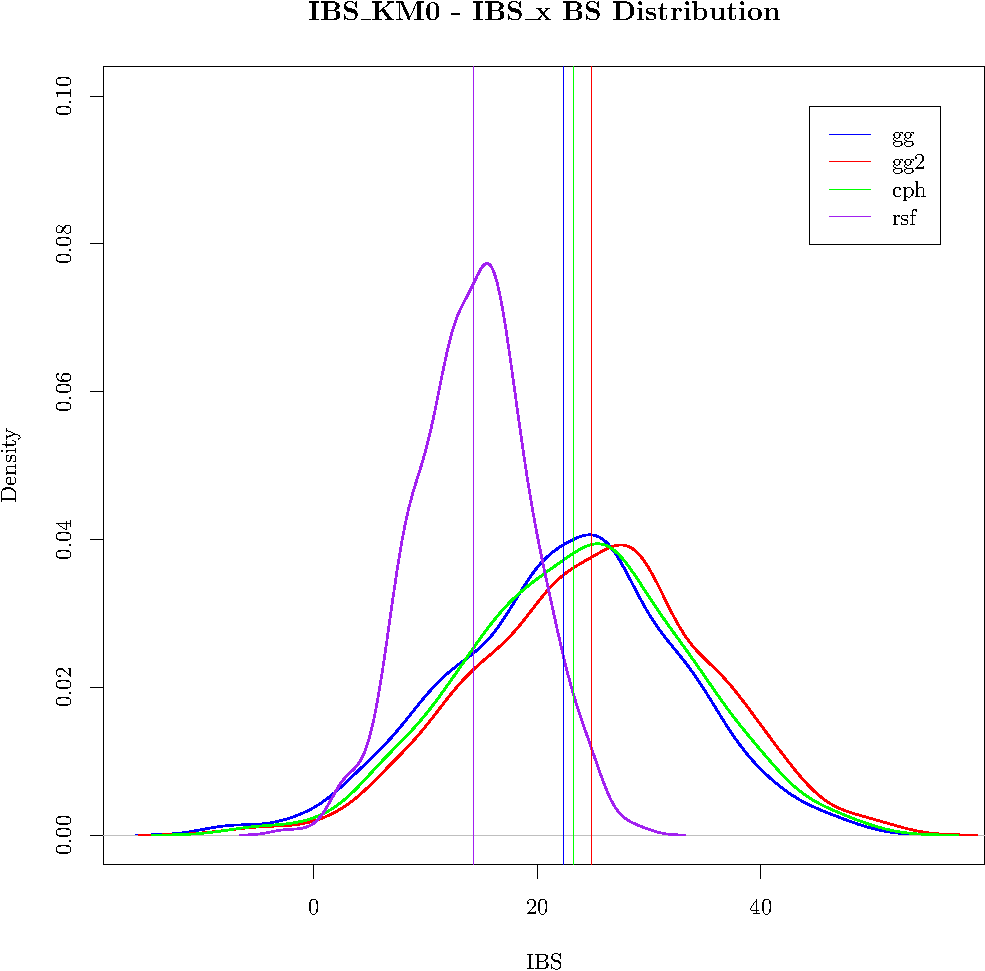
\includegraphics[width=\maxwidth]{figure/05-model-selection-ibs-3} 

}



\end{knitrout}

Do some proper BCA bootstrapping on the differences, just as a double-check test.
\begin{knitrout}
\definecolor{shadecolor}{rgb}{0.969, 0.969, 0.969}\color{fgcolor}\begin{kframe}
\begin{alltt}
\hlkwd{set.seed}\hlstd{(}\hlnum{20150208}\hlstd{)}
\hlstd{ibsc_boots2} \hlkwb{=} \hlkwd{boot}\hlstd{(data.val,} \hlkwc{statistic} \hlstd{=} \hlkwa{function}\hlstd{(}\hlkwc{d}\hlstd{,} \hlkwc{i}\hlstd{) \{}
        \hlstd{gg} \hlkwb{=} \hlkwd{calcIBS}\hlstd{(}\hlkwd{Surv}\hlstd{(d}\hlopt{$}\hlstd{Time, d}\hlopt{$}\hlstd{DSD)[i,], ibs_preds_gg[i,], ibs_times,} \hlnum{34}\hlopt{*}\hlnum{365.25}\hlopt{/}\hlnum{12}\hlstd{,} \hlnum{7}\hlopt{*}\hlnum{365.25}\hlopt{/}\hlnum{12}\hlstd{)}\hlopt{$}\hlstd{ibs}
        \hlstd{gg2} \hlkwb{=} \hlkwd{calcIBS}\hlstd{(}\hlkwd{Surv}\hlstd{(d}\hlopt{$}\hlstd{Time, d}\hlopt{$}\hlstd{DSD)[i,], ibs_preds_gg2[i,], ibs_times,} \hlnum{34}\hlopt{*}\hlnum{365.25}\hlopt{/}\hlnum{12}\hlstd{,} \hlnum{7}\hlopt{*}\hlnum{365.25}\hlopt{/}\hlnum{12}\hlstd{)}\hlopt{$}\hlstd{ibs}
        \hlstd{cph} \hlkwb{=} \hlkwd{calcIBS}\hlstd{(}\hlkwd{Surv}\hlstd{(d}\hlopt{$}\hlstd{Time, d}\hlopt{$}\hlstd{DSD)[i,], ibs_preds_cph[i,], ibs_times,} \hlnum{34}\hlopt{*}\hlnum{365.25}\hlopt{/}\hlnum{12}\hlstd{,} \hlnum{7}\hlopt{*}\hlnum{365.25}\hlopt{/}\hlnum{12}\hlstd{)}\hlopt{$}\hlstd{ibs}
        \hlstd{rsf} \hlkwb{=} \hlkwd{calcIBS}\hlstd{(}\hlkwd{Surv}\hlstd{(d}\hlopt{$}\hlstd{Time, d}\hlopt{$}\hlstd{DSD)[i,], ibs_preds_rsf[i,], ibs_times,} \hlnum{34}\hlopt{*}\hlnum{365.25}\hlopt{/}\hlnum{12}\hlstd{,} \hlnum{7}\hlopt{*}\hlnum{365.25}\hlopt{/}\hlnum{12}\hlstd{)}\hlopt{$}\hlstd{ibs}
        \hlstd{km0} \hlkwb{=} \hlkwd{calcIBS}\hlstd{(}\hlkwd{Surv}\hlstd{(d}\hlopt{$}\hlstd{Time, d}\hlopt{$}\hlstd{DSD)[i,], ibs_preds_km0[i,], ibs_times,} \hlnum{34}\hlopt{*}\hlnum{365.25}\hlopt{/}\hlnum{12}\hlstd{,} \hlnum{7}\hlopt{*}\hlnum{365.25}\hlopt{/}\hlnum{12}\hlstd{)}\hlopt{$}\hlstd{ibs}
        \hlkwd{c}\hlstd{(gg} \hlopt{-} \hlstd{km0, gg2} \hlopt{-} \hlstd{km0, cph} \hlopt{-} \hlstd{km0, rsf} \hlopt{-} \hlstd{km0, gg} \hlopt{-} \hlstd{rsf, gg2} \hlopt{-} \hlstd{rsf, cph} \hlopt{-} \hlstd{rsf, gg} \hlopt{-} \hlstd{cph, gg2} \hlopt{-} \hlstd{cph, gg} \hlopt{-} \hlstd{gg2)}
\hlstd{\},} \hlkwc{R} \hlstd{=} \hlnum{500}\hlstd{)}
\hlstd{ibsc_boots2_ci} \hlkwb{=} \hlkwd{t}\hlstd{(}\hlkwd{sapply}\hlstd{(}\hlnum{1}\hlopt{:}\hlkwd{length}\hlstd{(ibsc_boots2}\hlopt{$}\hlstd{t0),} \hlkwa{function}\hlstd{(}\hlkwc{i}\hlstd{)} \hlkwd{boot.ci}\hlstd{(ibsc_boots2,} \hlkwc{index} \hlstd{= i,} \hlkwc{type} \hlstd{=} \hlstr{"bca"}\hlstd{)}\hlopt{$}\hlstd{bca))}
\hlkwd{rownames}\hlstd{(ibsc_boots2_ci)} \hlkwb{=} \hlkwd{c}\hlstd{(}\hlstr{"gg-km0"}\hlstd{,} \hlstr{"gg2-km0"}\hlstd{,} \hlstr{"cph-km0"}\hlstd{,} \hlstr{"rsf-km0"}\hlstd{,} \hlstr{"gg-rsf"}\hlstd{,} \hlstr{"gg2-rsf"}\hlstd{,} \hlstr{"cph-rsf"}\hlstd{,} \hlstr{"gg-cph"}\hlstd{,} \hlstr{"gg2-cph"}\hlstd{,} \hlstr{"gg-gg2"}\hlstd{)}
\hlkwd{colnames}\hlstd{(ibsc_boots2_ci)} \hlkwb{=} \hlkwd{c}\hlstd{(}\hlstr{"level"}\hlstd{,} \hlstr{"orderi1"}\hlstd{,} \hlstr{"orderi2"}\hlstd{,} \hlstr{"lci"}\hlstd{,} \hlstr{"uci"}\hlstd{)}
\hlstd{ibsc_boots2}
\end{alltt}
\begin{verbatim}
## 
## ORDINARY NONPARAMETRIC BOOTSTRAP
## 
## 
## Call:
## boot(data = data.val, statistic = function(d, i) {
##     gg = calcIBS(Surv(d$Time, d$DSD)[i, ], ibs_preds_gg[i, ], 
##         ibs_times, 34 * 365.25/12, 7 * 365.25/12)$ibs
##     gg2 = calcIBS(Surv(d$Time, d$DSD)[i, ], ibs_preds_gg2[i, 
##         ], ibs_times, 34 * 365.25/12, 7 * 365.25/12)$ibs
##     cph = calcIBS(Surv(d$Time, d$DSD)[i, ], ibs_preds_cph[i, 
##         ], ibs_times, 34 * 365.25/12, 7 * 365.25/12)$ibs
##     rsf = calcIBS(Surv(d$Time, d$DSD)[i, ], ibs_preds_rsf[i, 
##         ], ibs_times, 34 * 365.25/12, 7 * 365.25/12)$ibs
##     km0 = calcIBS(Surv(d$Time, d$DSD)[i, ], ibs_preds_km0[i, 
##         ], ibs_times, 34 * 365.25/12, 7 * 365.25/12)$ibs
##     c(gg - km0, gg2 - km0, cph - km0, rsf - km0, gg - rsf, gg2 - 
##         rsf, cph - rsf, gg - cph, gg2 - cph, gg - gg2)
## }, R = 500)
## 
## 
## Bootstrap Statistics :
##      original   bias    std. error
## t1*   -21.062  1.16153      10.132
## t2*   -18.895  1.10126       9.319
## t3*   -20.209  1.14810       9.399
## t4*   -14.505  0.54879       5.156
## t5*    -6.557  0.61274       5.820
## t6*    -4.390  0.55247       5.219
## t7*    -5.704  0.59930       4.888
## t8*    -0.853  0.01344       2.103
## t9*     1.314 -0.04683       4.374
## t10*   -2.167  0.06027       5.015
\end{verbatim}
\begin{alltt}
\hlstd{ibsc_boots2_ci}
\end{alltt}
\begin{verbatim}
##         level orderi1 orderi2     lci    uci
## gg-km0   0.95    8.84   483.4 -42.087 -2.195
## gg2-km0  0.95    6.04   477.0 -39.834 -2.575
## cph-km0  0.95    4.95   473.6 -41.625 -4.555
## rsf-km0  0.95    3.86   469.0 -26.894 -6.234
## gg-rsf   0.95    9.64   484.5 -17.396  4.837
## gg2-rsf  0.95   14.55   490.4 -13.874  6.460
## cph-rsf  0.95    7.02   479.6 -15.948  2.835
## gg-cph   0.95   19.34   493.6  -4.524  4.448
## gg2-cph  0.95   13.62   489.5  -6.992 10.142
## gg-gg2   0.95   16.42   491.8 -11.578  9.249
\end{verbatim}
\end{kframe}
\end{knitrout}
All models perform equivalently on the validation set.  Select the simplest: gg.


%%%%%%%%%%%%%%%%%%%%%%%%%%%%%%%%%%%%%%%%%%%%%%%%%%%%%%%%%%%%%%%%%%%%%%
% CALCULATE AND SAVE FINAL MODEL
%%%%%%%%%%%%%%%%%%%%%%%%%%%%%%%%%%%%%%%%%%%%%%%%%%%%%%%%%%%%%%%%%%%%%%
Final model fitting:
\begin{knitrout}
\definecolor{shadecolor}{rgb}{0.969, 0.969, 0.969}\color{fgcolor}\begin{kframe}
\begin{alltt}
\hlstd{data.all} \hlkwb{=} \hlkwd{rbind}\hlstd{(data[}\hlkwd{colnames}\hlstd{(data.val)], data.val)}
\hlkwd{head}\hlstd{(data.all)}
\end{alltt}
\begin{verbatim}
##           Time  DSD DiagYearCent  SexM AgeCent LocBody SizeCent    A2   A4
## NSWPCN_4   937 TRUE       -5.717  TRUE     -16   FALSE       -1 FALSE TRUE
## NSWPCN_9   587 TRUE       -7.173  TRUE       5   FALSE       10 FALSE TRUE
## NSWPCN_10  177 TRUE       -7.337  TRUE      -9   FALSE       10 FALSE TRUE
## NSWPCN_13  247 TRUE       -7.532 FALSE     -19    TRUE       20 FALSE TRUE
## NSWPCN_17  316 TRUE       -7.417 FALSE     -23   FALSE       -5 FALSE TRUE
## NSWPCN_20  256 TRUE       -3.392 FALSE      -8   FALSE        0 FALSE TRUE
##           SizePlus
## NSWPCN_4         0
## NSWPCN_9        10
## NSWPCN_10       10
## NSWPCN_13       20
## NSWPCN_17        0
## NSWPCN_20        0
\end{verbatim}
\begin{alltt}
\hlcom{#fit.final.gg = flexsurvreg(Surv(Time, DSD) ~ SexM + AgeCent + LocBody + SizeCent + A2 + A4 + SizeCent:AgeCent + SexM:SizeCent,}
\hlstd{fit.final.gg} \hlkwb{=} \hlkwd{flexsurvreg}\hlstd{(}\hlkwd{Surv}\hlstd{(Time, DSD)} \hlopt{~} \hlstd{SexM} \hlopt{+} \hlstd{LocBody} \hlopt{+} \hlstd{SizeCent} \hlopt{+} \hlstd{A2} \hlopt{+} \hlstd{A4,}
        \hlkwc{anc} \hlstd{=} \hlkwd{list}\hlstd{(}
                \hlkwc{sigma} \hlstd{=} \hlopt{~} \hlstd{SexM,}
                \hlkwc{Q} \hlstd{=} \hlopt{~} \hlstd{SexM),}
        \hlkwc{data} \hlstd{= data.all,} \hlkwc{dist} \hlstd{=} \hlstr{"gengamma"}\hlstd{)}
\hlcom{# fit.final.cph = coxph(Surv(Time, DSD) ~ strata(SexM)+AgeCent+LocBody+SizeCent+A2+A4+SizeCent:AgeCent+strata(SexM):SizeCent, data = data.all, x = TRUE, y = TRUE, model = TRUE)}
\hlstd{fit.final.cph} \hlkwb{=} \hlkwd{coxph}\hlstd{(}\hlkwd{Surv}\hlstd{(Time, DSD)} \hlopt{~} \hlkwd{strata}\hlstd{(SexM)} \hlopt{+} \hlstd{LocBody} \hlopt{+} \hlstd{SizeCent} \hlopt{+} \hlstd{A2} \hlopt{+} \hlstd{A4,} \hlkwc{data} \hlstd{= data.all,} \hlkwc{x} \hlstd{=} \hlnum{TRUE}\hlstd{,} \hlkwc{y} \hlstd{=} \hlnum{TRUE}\hlstd{,} \hlkwc{model} \hlstd{=} \hlnum{TRUE}\hlstd{)}
\hlkwd{set.seed}\hlstd{(}\hlnum{20150208}\hlstd{)}
\hlstd{fit.final.rsf} \hlkwb{=} \hlkwd{rfsrc}\hlstd{(}\hlkwd{Surv}\hlstd{(Time, DSD)} \hlopt{~} \hlstd{SexM} \hlopt{+} \hlstd{AgeCent} \hlopt{+} \hlstd{LocBody} \hlopt{+} \hlstd{SizeCent} \hlopt{+} \hlstd{A2} \hlopt{+} \hlstd{A4,} \hlkwc{data} \hlstd{= data.all,} \hlkwc{mtry} \hlstd{=} \hlnum{1}\hlstd{,} \hlkwc{splitrule} \hlstd{=} \hlstr{"logrankscore"}\hlstd{,} \hlkwc{nsplit} \hlstd{=} \hlnum{2}\hlstd{,} \hlkwc{ntree} \hlstd{=} \hlnum{1000}\hlstd{)}
\hlstd{fit.final.km0} \hlkwb{=} \hlkwd{survfit}\hlstd{(}\hlkwd{Surv}\hlstd{(Time, DSD)} \hlopt{~} \hlnum{1}\hlstd{, data.all)}
\hlkwd{saveRDS}\hlstd{(}\hlkwd{list}\hlstd{(}\hlkwc{gg} \hlstd{= fit.final.gg,} \hlkwc{km0} \hlstd{= fit.final.km0,} \hlkwc{cph} \hlstd{= fit.final.cph,} \hlkwc{rsf} \hlstd{= fit.final.rsf,} \hlkwc{data.train} \hlstd{= data.all),} \hlkwc{file} \hlstd{=} \hlstr{"05_final_model.rds"}\hlstd{)}
\end{alltt}
\end{kframe}
\end{knitrout}

\begin{knitrout}
\definecolor{shadecolor}{rgb}{0.969, 0.969, 0.969}\color{fgcolor}\begin{kframe}
\begin{alltt}
\hlkwd{save.image}\hlstd{(}\hlstr{"05_train_NSWPCN_2.rda"}\hlstd{)}
\end{alltt}
\end{kframe}
\end{knitrout}

%%%%%%%%%%%%%%%%%%%%%%%%%%%%%%%%%%%%%%%%%%%%%%%%%%%%%%%%%%%%%%%%%%%%%%
% THE END
%%%%%%%%%%%%%%%%%%%%%%%%%%%%%%%%%%%%%%%%%%%%%%%%%%%%%%%%%%%%%%%%%%%%%%
\section{Session information}
\begin{knitrout}
\definecolor{shadecolor}{rgb}{0.969, 0.969, 0.969}\color{fgcolor}\begin{kframe}
\begin{alltt}
\hlkwd{sessionInfo}\hlstd{()}
\end{alltt}
\begin{verbatim}
## R version 3.1.1 (2014-07-10)
## Platform: x86_64-unknown-linux-gnu (64-bit)
## 
## locale:
##  [1] LC_CTYPE=en_AU.UTF-8          LC_NUMERIC=C                 
##  [3] LC_TIME=en_AU.UTF-8           LC_COLLATE=en_AU.UTF-8       
##  [5] LC_MONETARY=en_AU.UTF-8       LC_MESSAGES=en_AU.UTF-8      
##  [7] LC_PAPER=en_AU.UTF-8          LC_NAME=en_AU.UTF-8          
##  [9] LC_ADDRESS=en_AU.UTF-8        LC_TELEPHONE=en_AU.UTF-8     
## [11] LC_MEASUREMENT=en_AU.UTF-8    LC_IDENTIFICATION=en_AU.UTF-8
## 
## attached base packages:
## [1] parallel  methods   splines   stats     graphics  grDevices utils    
## [8] datasets  base     
## 
## other attached packages:
##  [1] RColorBrewer_1.0-5    timeROC_0.2           timereg_1.8.6        
##  [4] mvtnorm_1.0-1         pec_2.4.4             boot_1.3-13          
##  [7] MASS_7.3-35           ggplot2_1.0.0         plyr_1.8.1           
## [10] reshape2_1.4          randomForestSRC_1.5.5 flexsurv_0.5         
## [13] glmulti_1.0.7         rJava_0.9-6           survival_2.37-7      
## [16] tikzDevice_0.8.1      knitr_1.8            
## 
## loaded via a namespace (and not attached):
##  [1] codetools_0.2-9  colorspace_1.2-4 deSolve_1.11     digest_0.6.4    
##  [5] evaluate_0.5.5   filehash_2.2-2   foreach_1.4.2    formatR_1.0     
##  [9] grid_3.1.1       gtable_0.1.2     highr_0.4        iterators_1.0.7 
## [13] labeling_0.3     lava_1.3         muhaz_1.2.6      munsell_0.4.2   
## [17] prodlim_1.5.1    proto_0.3-10     Rcpp_0.11.3      scales_0.2.4    
## [21] stringr_0.6.2    tools_3.1.1
\end{verbatim}
\end{kframe}
\end{knitrout}

\end{document}



